\chapter{薄板问题HR}
本章进一步针对薄板问题,基于Hellinger-Reissner变分原理提出了一种满足变分一致性的伽辽金无网格法。首先介绍了薄板问题时Hellinger-Reissner变分原理及其所提方法的混合离散过程,
其次介绍该方法的本质边界条件施加过程并与传统Nitsche法进行对比,最后通过薄板算例验证该方法的变分一致性、计算精度和计算效率
\section{Hellinger-Reissner变分原理}
根据最小余能原理,薄板问题强形式(\ref{P control equation})所对应的余能泛函表达式为:
\begin{equation}
\Pi_C(M_{\alpha\beta})=\int_{\Omega}\frac{1}{2}M_{\alpha\beta}C^{-1}_{\alpha\beta\gamma\eta}M_{\gamma\eta}d\Omega-\int_{\Gamma_w}V_{\pmb n}\bar{w}d\Gamma+\int_{\Gamma_{\theta}}M_{\pmb{nn}}\bar{\theta}_nd\Gamma-p\bar{w}\vert_{x\in{c_w}}
\end{equation}
与弹性力学问题类似,薄板问题的Hellinger-Reissner变分原理余能泛函具有挠度和弯矩两个变量\cite{},四阶薄板问题控制方程式(\ref{P control equation})对应的余能泛函表达式为:
\begin{equation}\label{pfanhan}
\begin{split}
    \Pi_{H\!R}(M_{\alpha\beta},w)&=\Pi_C(M_{\alpha\beta})+\int_{\Omega}w(M_{\alpha\beta,\alpha\beta}+\bar{q})d\Omega\\
    &+\int_{\Gamma_M}w_{,\pmb n}(M_{\pmb{nn}}-\bar{M}_{\pmb{nn}})d\Gamma
    -\int_{\Gamma_V}w(V_{\pmb n}-\bar{V}_{\pmb n})d\Gamma-w(P-\bar{P})\vert_{x\in{c_P}}
\end{split}
\end{equation}
式(\ref{pfanhan})分别对$M_{\alpha\beta}$和$w$进行变分得到薄板问题Hellinger-Reissner变分原理的伽辽金弱形式:
\begin{equation}\label{Pweakfrom}
\begin{split}
    \delta\Pi_{H\!R}(M_{\alpha\beta,w})=&\delta\Pi_C(M_{\alpha\beta})\\
    &+\int_{\Omega}\delta M_{\alpha\beta,\alpha\beta}wd\Omega+\int_{\Gamma_M}\delta M_{\pmb{nn}}w_{,\pmb n}d\Gamma-\int_{\Gamma_V}\delta V_{\pmb n}wd\Gamma-\delta Pw\vert_{x\in{c_P}}\\
    &+\int_{\Omega}\delta w(M_{\alpha\beta,\alpha\beta}+\bar{q})d\Omega+\int_{\Gamma_M}\delta w_{,n}(M_{nn}-\bar{M}_{nn})d\Gamma\\
    &-\int_{\Gamma_V}\delta w(V_{\pmb n}-\bar{V}_{\pmb n})d\Gamma-\delta w(P-\bar{P})\vert_{x\in{c_P}}\\
    &=0
\end{split}
\end{equation}\par
根据变分项$\delta M_{\alpha\beta}$和$\delta w$的任意性和几何关系式(\ref{PGeometric relationships})进一步将上式改写为以下两式:
\begin{equation}\label{Pweakform1}
    \begin{split}
        \int_\Omega {\delta {M_{\alpha \beta }}D_{\alpha \beta \gamma \eta }^{ - 1}{M_{\gamma \eta }}d\Omega }&=\int_\Gamma  {\delta {V_{\bf{n}}}wd\Gamma }  - \int_\Gamma  {\delta {M_{{\bf{nn}}}}{w_{,{\bf{n}}}}d\Gamma }+{\left. {\delta Pw} \right|_{{\bf{x}} \in c}} - \int_\Omega  {\delta {M_{\alpha \beta ,\alpha \beta }}wd\Omega } \\
        &-\int_{{\Gamma _w}} {\delta {V_{\bf{n}}}wd\Gamma }  + \int_{{\Gamma _\theta }} {\delta {M_{{\bf{nn}}}}{w_{,{\bf{n}}}}d\Gamma }  - {\left. {\delta Pw} \right|_{{\bf{x}} \in {c_w}}}\\
        &+\int_{{\Gamma _w}} {\delta {V_{\bf{n}}}\bar wd\Gamma }  - \int_{{\Gamma _\theta }} {\delta {M_{{\bf{nn}}}}{{\bar \theta }_{\bf{n}}}d\Gamma }  + {\left. {\delta P\bar w} \right|_{{\bf{x}} \in {c_w}}}
    \end{split}
\end{equation}
\begin{equation}
        \begin{split}\label{Pweakform2}
            &\int_\Gamma  {\delta w{V_{\bf{n}}}d\Gamma } - \int_\Gamma  {\delta {w_{,{\bf{n}}}}{M_{{\bf{nn}}}}d\Gamma }  + {\left. {\delta wP} \right|_{{\bf{x}} \in c}} - \int_\Omega  {\delta w{M_{\alpha \beta ,\alpha\beta}}d\Omega }\\
            &- \int_{{\Gamma _w}} {\delta w{V_{\bf{n}}}d\Gamma }  + \int_{{\Gamma _\theta }} {\delta {w_{,{\bf{n}}}}{M_{{\bf{nn}}}}d\Gamma }  - {\left. {\delta wP} \right|_{{\bf{x}} \in {c_w}}}\\
            &= \int_{{\Gamma _V}} {\delta w{{\bar V}_{\bf{n}}}d\Gamma }  - \int_{{\Gamma _M}} {\delta {w_{,{\bf{n}}}}{{\bar M}_{{\bf{nn}}}}d\Gamma }  + {\left. {\delta w\bar P} \right|_{{\bf{x}} \in {c_P}}} + \int_\Omega  {\delta w\bar qd\Omega} 
    \end{split}
\end{equation} 
\section{挠度-弯矩混合离散}
Hellinger-Reissner变分原理薄板弱形式中的挠度和弯矩采用混合离散进行近似。
首先,薄板挠度$w$采用无网格形函数(\ref{Pshapefunction})进行近似离散,近似的挠度$w^h$表达式可表示为:
\begin{equation}\label{w}
    w^h(\pmb{x})=\sum_{I=1}^{N\!P}\Psi_I(\pmb{x})d_{I}
\end{equation}
其中$d_I$表示与无网格节点$\pmb{x}_I$对应的节点系数。\par
其次,弯矩分量$M_{\alpha\beta}$在每个背景积分域内假设为$(p-2)$阶多项式。
如图(\ref{Pintegralscheme})所示,将薄板中面$\Omega$划分为一系列背景积分域$\Omega_C,C=1,2,\dotsb,n_C$,并且存在$\cup_{C=1}^{N\!C}\Omega_C\thickapprox\Omega$。
在背景积分单元$\Omega_C$内,假定弯矩分量$M_{\alpha\beta}$为多项式,近似的弯矩分量$M_{\alpha\beta}^h$:
\begin{equation}\label{moment}
\begin{split}
    M^h_{\alpha\beta}(\pmb{x})=\pmb{a}_{\alpha\beta}^T\pmb{p}^{[p-2]}(\pmb{x})
\end{split}
\end{equation}
其中$\pmb{p}^{[p-2]}(\pmb x)$是$(p-2)$阶的单项式向量,$\pmb{a}_{\alpha\beta}$为弯矩分量$M_{\alpha\beta}$在积分域$\Omega_C$内的常系数向量。此时将离散的弯矩分量表达式(\ref{moment})代入式(\ref{Pweakform1})同时根据式(\ref{MVP})和线弹性本构关系式(\ref{Malphabeta})可以得到:
\begin{equation}
\begin{split}
    &\int_{\Omega}\delta\pmb{a}_{\alpha\beta}^T\pmb{p}^{[p-2]}D^{-1}_{\alpha\beta\gamma\eta}\pmb{a}_{\gamma\eta}^T\pmb{p}^{[p-2]}d\Omega=\\
    &-\int_{\Gamma}D_{\alpha\beta\gamma\eta}^{-1}\mathcal{V}_{\alpha\beta}\delta\pmb{a}_{,\alpha\beta}^T\pmb{p}^{[p-2]}wd\Gamma
    +\int_{\Gamma}D_{\alpha\beta\gamma\eta}^{-1}\mathcal{M}_{\alpha\beta}\delta\pmb{a}_{,\alpha\beta}^T\pmb{p}^{[p-2]}w_{,\pmb{n}}d\Gamma\\
    &-D_{\alpha\beta\gamma\eta}^{-1}\mathcal{P}_{\alpha\beta}\delta\pmb{a}_{,\alpha\beta}^T\pmb{p}^{[p-2]}w\vert_{x\in c}
    -\int_{\Omega}\delta\pmb{a}_{\alpha\beta,\alpha\beta}^T\pmb{p}^{[p-2]}wd\Omega\\
    &+\int_{\Gamma_w}D_{\alpha\beta\gamma\eta}^{-1}\mathcal{V}_{\alpha\beta}\delta\pmb{a}_{,\alpha\beta}^T\pmb{p}^{[p-2]}d\Gamma
    -\int_{\Gamma_{\theta}}D_{\alpha\beta\gamma\eta}^{-1}\mathcal{M}_{\alpha\beta}\delta\pmb{a}_{,\alpha\beta}^T\pmb{p}^{[p-2]}w_{,\pmb{n}}d\Gamma\\
    &+D_{\alpha\beta\gamma\eta}^{-1}\mathcal{P}_{\alpha\beta}\delta\pmb{a}_{,\alpha\beta}^T\pmb{p}^{[p-2]}wx\vert_{x\in{c_w}}
    -\int_{\Gamma_w}D_{\alpha\beta\gamma\eta}^{-1}\mathcal{V}_{\alpha\beta}\delta\pmb{a}_{,\alpha\beta}^T\pmb{p}^{[p-2]}\bar{w}d\Gamma\\
    &+\int_{\Gamma_{\theta}}D_{\alpha\beta\gamma\eta}^{-1}\mathcal{M}_{\alpha\beta}\delta\pmb{a}_{,\alpha\beta}^T\pmb{p}^{[p-2]}\bar{\theta}_{\pmb{n}}d\Gamma
    -D_{\alpha\beta\gamma\eta}^{-1}\mathcal{P}_{\alpha\beta}\delta\pmb{a}_{,\alpha\beta}^T\pmb{p}^{[p-2]}\bar{w}\vert_{x\in{c_w}}
\end{split}
\end{equation}
进一步将等式两边同时消去$\delta\pmb{a}^T_{\alpha\beta}$得到:
\begin{equation}
\begin{split}
        &\int_{\Omega}\pmb{p}^{[p-2]}D^{-1}_{\alpha\beta\gamma\eta}\pmb{a}_{\gamma\eta}^T\pmb{p}^{[p-2]}d\Omega=\\
        &-\int_{\Gamma}D_{\alpha\beta\gamma\eta}^{-1}\mathcal{V}_{\alpha\beta}\pmb{p}^{[p-2]}wd\Gamma
        +\int_{\Gamma}D_{\alpha\beta\gamma\eta}^{-1}\mathcal{M}_{\alpha\beta}\pmb{p}^{[p-2]}w_{,\pmb{n}}d\Gamma\\
        &-D_{\alpha\beta\gamma\eta}^{-1}\mathcal{P}_{\alpha\beta}\pmb{p}^{[p-2]}w\vert_{x\in c}
        -\int_{\Omega}\delta\pmb{a}_{\alpha\beta,\alpha\beta}^T\pmb{p}^{[p-2]}wd\Omega\\
        &+\int_{\Gamma_w}D_{\alpha\beta\gamma\eta}^{-1}\mathcal{V}_{\alpha\beta}\pmb{p}^{[p-2]}d\Gamma
        -\int_{\Gamma_{\theta}}D_{\alpha\beta\gamma\eta}^{-1}\mathcal{M}_{\alpha\beta}\pmb{p}^{[p-2]}w_{,\pmb{n}}d\Gamma\\
        &+D_{\alpha\beta\gamma\eta}^{-1}\mathcal{P}_{\alpha\beta}\pmb{p}^{[p-2]}wx\vert_{x\in{c_w}}
        -\int_{\Gamma_w}D_{\alpha\beta\gamma\eta}^{-1}\mathcal{V}_{\alpha\beta}\pmb{p}^{[p-2]}\bar{w}d\Gamma\\
        &+\int_{\Gamma_{\theta}}D_{\alpha\beta\gamma\eta}^{-1}\mathcal{M}_{\alpha\beta}\pmb{p}^{[p-2]}\bar{\theta}_{\pmb{n}}d\Gamma
        -D_{\alpha\beta\gamma\eta}^{-1}\mathcal{P}_{\alpha\beta}\pmb{p}^{[p-2]}\bar{w}\vert_{x\in{c_w}}
\end{split}
\end{equation}
对上式进行移项可以得到常系数向量$\pmb{a}_{\alpha\beta}$的具体表达式:
\begin{equation}\label{aalphabeta}
\begin{split}
    \pmb{a}_{\gamma\eta}=-D_{\alpha\beta\gamma\eta}\pmb{G}^{-1}(\sum_{I=1}^{N\!P}(\tilde{\pmb g}_{\alpha\beta I}-\bar{\pmb g}_{\alpha\beta I})d_I+\hat{\pmb g}_{\alpha\beta})
\end{split}
\end{equation}
其中
\begin{align}
\label{PG}\pmb{G}&=\int_{\Omega_C}\pmb{p}^{[p-2]}\pmb{p}^{[p-2]T}d\Omega\\
\label{Pg1}\tilde{\pmb g}_{\alpha\beta I}&=\int_{\Gamma_C}\Psi_{I,n}\pmb{p}^{[p-2]}n_{\alpha}n_{\beta}d\Gamma-\int_{\Gamma_C}\Psi_I(n_{\alpha}\pmb{p}^{[p-2]}_{,\beta}+\pmb{p}^{[p-2]}_{,\gamma}s_{\alpha}n_{\beta}s_{\gamma})d\Gamma \nonumber\\
&+[[\Psi_I\pmb{p}^{[p-2]}n_{\alpha}s_{\beta}]]\vert_{x\in c_C}+\int_{\Omega_C}\Psi_I\pmb{p}^{[p-2]}_{,\alpha\beta}d\Omega\\
\label{Pg2}\bar{\pmb g}_{\alpha\beta I}&=\int_{{\Gamma_{\theta}}\cap{\Gamma_C}}\Psi_{I,n}\pmb{p}^{[p-2]}n_{\alpha}n_{\beta}d\Gamma-\int_{{\Gamma_w}\cap{\Gamma_C}}\Psi_I(n_{\alpha}\pmb{p}^{[p-2]}_{,\beta}+\pmb{p}^{[p-2]}_{,\gamma}s_{\alpha}n_{\beta}s_{\gamma})d\Gamma\nonumber\\
&+[[\Psi_I\pmb{p}^{[p-2]}n_{\alpha}s_{\beta}]]\vert_{x\in{c_w}\cap{c_C}}\\
\label{Pg3}\hat{\pmb g}_{\alpha\beta I}&=\int_{{\Gamma_{\theta}}\cap{\Gamma_C}}\pmb{p}^{[p-2]}n_{\alpha}n_{\beta}\bar{\theta}_nd\Gamma-\int_{{\Gamma_w}\cap{\Gamma_C}}(n_{\alpha}\pmb{p}^{[p-2]}_{,\beta}+\pmb{p}^{[p-2]}_{,\gamma}s_{\alpha}n_{\beta}s_{\gamma})\bar{w}d\Gamma\nonumber\\
&+[[\bar{w}\pmb{p}^{[p-2]}n_{\alpha}s_{\beta}]]\vert_{x\in{c_w}\cap{c_C}}
\end{align}
式中$\Gamma_C$是$\Omega_C$的边界,此时将$\pmb{a}_{\alpha\beta}$代入到式(\ref{moment})中得到近似的弯矩分量$M^h_{\alpha\beta}(\pmb{x})$的表达式:
\begin{equation}
\begin{split}
M^h_{\alpha\beta}(\pmb{x})&=\pmb{p}^{[p-2]T}(\pmb{x})\pmb a_{\alpha\beta}\\
&=-D_{\alpha\beta\gamma\eta}(\sum_{I=1}^{N\!P}\pmb{p}^{[p-2]T}(\pmb x)\pmb G^{-1}\tilde{\pmb g}_{\gamma\eta I}-\pmb{p}^{[p-2]T}(\pmb x)\pmb G^{-1}\bar{\pmb g}_{\gamma\eta I})d_I+\pmb{p}^{[p-2]T}(\pmb x)\pmb G^{-1}\hat{\pmb g}_{\gamma\eta})\\
&=-D_{\alpha\beta\gamma\eta}(\sum_{I=1}^{N\!P}\tilde{\Psi}_{I,\gamma\eta}(\pmb x)d_I-\sum_{I=1}^{N\!P}\bar{\Psi}_{I,\gamma\eta}(\pmb{x})d_I+\pmb{p}^{[p-2]T}(\pmb x)\pmb G^{-1}\hat{\pmb g}_{\gamma\eta})
\end{split}
\end{equation}
其中
\begin{align}
 \label{PTPSI}&\tilde{\Psi}_{I,\alpha\beta}=\pmb{p}^{[p-2]T}(\pmb x)\pmb G^{-1}\tilde{\pmb g}_{\alpha\beta I}\\
 \label{PBPSI}&\bar{\Psi}_{I,\alpha\beta}=\pmb{p}^{[p-2]T}(\pmb x)\pmb G^{-1}\bar{\pmb g}_{\alpha\beta I}
\end{align}\par
此时,弯矩分量表达式中的$\tilde{\Psi}_{I,\alpha\beta}$是根据再生光滑梯度理论\cite{}构造的二阶再生光滑梯度。
根据再生光滑梯度理论框架,直接通过无网格形函数显式构造再生光滑梯度,可以避免传统无网格形函数梯度的复杂计算从而提高梯度计算效率。
$\tilde{\pmb g}_{\alpha\beta I}$是指在薄板问题中由再生光滑梯度法内嵌的局部积分约束条件,在求解高阶薄板问题时可以保证算法的计算精度和误差收敛性。
表示在求解薄板问题时,可以通过构造再生光滑梯度,保证误差收敛性提高计算精度。
\begin{figure}[H]
    \centering
    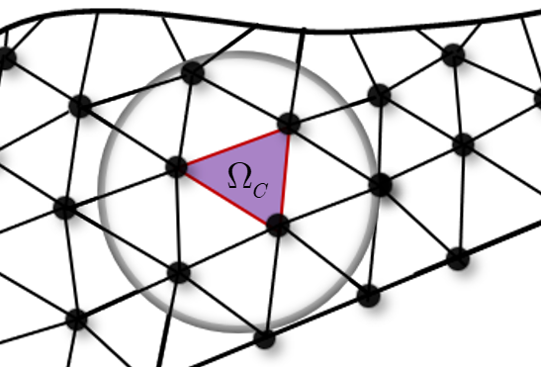
\includegraphics[scale=0.5]{figure/PHR/momentlisan.png}
    \caption{背景积分域示意图}\label{Pintegralscheme}
\end{figure}
\section{Hellinger-Reissner变分原理下的本质边界条件施加方法}
基于Hellinger-Reissner变分原理的薄板问题伽辽金弱形式(\ref{Pweakform})中的积分项包括了在本质边界条件下的弯矩的约束项,以及在自然边界条件下的挠度和集中荷载外力项。
此时,通过对挠度采用再生核近似,弯矩通过局部多项式近似的混合离散方式对Hellinger-Reissner变分原理的薄板问题等效积分弱形式进行组装刚度矩阵。
首先,将挠度离散表达式(\ref{w})和弯矩离散表达式(\ref{moment})代入到弱形式(\ref{Pweakform2})中得到:
\begin{equation}\label{CH5-1}
\begin{split}
    &\int_{\Gamma}\sum_{I=1}^{N\!P}\Psi_I\delta{d_I}\mathcal{V}_{\alpha\beta}w_{,\alpha\beta}d\Gamma-\int_{\Gamma}\sum_{I=1}^{N\!P}\Psi_{I,n}\delta{d_I}\mathcal{M}_{\alpha\beta}w_{,\alpha\beta}d\Gamma+\sum_{I=1}^{N\!P}\Psi_I\delta{d_I}\mathcal{P}_{\alpha\beta}w_{,\alpha\beta}\vert_{x\in c}\\
    &-\int_{\Omega}\sum_{I=1}^{N\!P}\Psi_I\delta{d_I}\pmb{a}^T_{\alpha\beta,\alpha\beta}\pmb{p}^{[p-2]}d\Omega-\int_{\Gamma_w}\sum_{I=1}^{N\!P}\Psi_I\delta{d_I}\mathcal{V}_{\alpha\beta}w_{,\alpha\beta}d\Gamma\\
    &+\int_{\Gamma_{\theta}}\sum_{I=1}^{N\!P}\Psi_{I,n}\delta{d_I}\mathcal{M}_{\alpha\beta}w_{,\alpha\beta}d\Gamma
    -\sum_{I=1}^{N\!P}\Psi_I\delta{d_I}\mathcal{P}_{\alpha\beta}w_{,\alpha\beta}\vert_{x\in c_w}\\
    &=\sum_{I=1}^{N\!P}\int_{\Gamma_V}\Psi_I\delta{d_I}\bar{V}_{\pmb n}d\Gamma-\sum_{I=1}^{N\!P}\int_{\Gamma_M}\Psi_{I,n}\delta{d_I}\bar{M}_{\pmb{nn}}d\Gamma
    +\sum_{I=1}^{N\!P}\Psi_I\delta{d_I}\bar{P}\vert_{x\in{c_P}}+\sum_{I=1}^{N\!P}\int_{\Omega}\Psi_I\delta{d_I}\bar{q}d\Omega
\end{split}
\end{equation}
其次引入式(\ref{MVP1})并根据薄板问题线弹性本构关系式(\ref{Malphabeta})将上式改写为:
\begin{equation}\label{CH5-2}
\begin{split}
  -\sum_{C=1}^{N\!C}(\tilde{\pmb g}_{\alpha\beta I}^T-\bar{\pmb g}_{\alpha\beta I}^T)\pmb a_{\alpha\beta}=\pmb{f}
\end{split}
\end{equation}
进一步再将式(\ref{aalphabeta})中的$\pmb{a}_{\alpha\beta}$代入到式(\ref{CH5-2})中进而得到:
\begin{equation}
\begin{split}\label{Pzuzhuang}
    &-\sum_{C=1}^{N\!C}(\tilde{\pmb g}_{\alpha\beta I}^T-\bar{\pmb g}_{\alpha\beta I}^T)\pmb a_{\alpha\beta}\\
    &=\sum_{C=1}^{N\!C}(\tilde{\pmb g}_{\alpha\beta I}^T-\bar{\pmb g}_{\alpha\beta I}^T)D_{\alpha\beta\gamma\eta}\pmb{G}^{-1}(\sum_{J=1}^{N\!P}(\tilde{\pmb g}_{\gamma\eta J}-\bar{\pmb g}_{\gamma\eta J})d_I+\hat{\pmb g}_{\gamma\eta})\\
    &=\sum_{C=1}^{N\!C}
    \left(\begin{split}
    &\sum_{J=1}^{N\!P}\underbrace{D_{\alpha\beta\gamma\eta}\tilde{\pmb g}_{\alpha\beta I}^T\pmb G^{-1}\tilde{\pmb g}_{\gamma\eta J}}_{\pmb{K}}d_J\\
    &+\sum_{J=1}^{N\!P}\underbrace{D_{\alpha\beta\gamma\eta}(-\bar{\pmb g}_{\alpha\beta I}^T\pmb G^{-1}\tilde{\pmb g}_{\gamma\eta J}-\tilde{\pmb g}_{\alpha\beta I}^T\pmb G^{-1}\tilde{\pmb g}_{\gamma\eta J})}_{\tilde{\pmb K}}d_J\\
    &+\sum_{J=1}^{N\!P}\underbrace{D_{\alpha\beta\gamma\eta}\bar{\pmb g}_{\alpha\beta I}^T\pmb G^{-1}\tilde{\pmb g}_{\gamma\eta J}}_{\bar{\pmb K}}d_J\\
    &-\underbrace{(-D_{\alpha\beta\gamma\eta}\tilde{\pmb g}_{\alpha\beta I}^T\pmb G^{-1}\hat{\pmb g}_{\gamma\eta })}_{\tilde{\pmb f}}\\
    &-\underbrace{D_{\alpha\beta\gamma\eta}\bar{\pmb g}_{\alpha\beta I}^T\pmb G^{-1}\hat{\pmb g}_{\gamma\eta }}_{\bar{\pmb f}}\\
    \end{split}\right)\\
    &=\sum_{J=1}^{N\!P}(\pmb{K}+\tilde{\pmb{K}}+\bar{\pmb{K}})\pmb d_J-\tilde{\pmb f}-\bar{\pmb f}
\end{split}
\end{equation}
式中的最后一个等式通过引入式(\ref{PG})-(\ref{PBPSI})和(\ref{MVP})进行化简得到,具体详细的推导可参考\nameref{B}。根据式(\ref{CH5-2})和(\ref{Pzuzhuang})代入到式(\ref{CH5-1})中可得到Hellinger-Reissner变分原理下的薄板问题离散控制方程:
\begin{equation}\label{equationP}
    (\pmb{K}+\tilde{\pmb K}+\bar{\pmb K})\pmb{d}=\pmb{f}+\tilde{\pmb f}+\bar{\pmb f}
\end{equation}
其中刚度矩阵$\pmb K$、$\tilde{\pmb K}$和$\bar{\pmb K}$,力向量$\pmb f$、$\tilde{\pmb f}$和$\bar{\pmb f}$的具体表达式如下:
\begin{subequations}\label{PHR1}
\begin{align}
K_{IJ}&=\int_{\Omega}\tilde{\Psi}_{I,\alpha\beta}D_{\alpha\beta\gamma\eta}\tilde{\Psi}_{J,\gamma\eta}d\Omega \\
f_I&=\int_{\Gamma_V}\Psi_I\bar{V}_{\pmb{n}}d\Gamma-\int_{\Gamma_M}\Psi_{I,\pmb{n}}\bar{M}_{\pmb{nn}}d\Gamma+\Psi_I\bar{P}\vert_{x\in c_P}+\int_{\Omega}\Psi_I\bar{q}d\Omega
\end{align}
\end{subequations}
\begin{subequations}\label{PHR2}
\begin{align}
  \tilde{K}_{IJ}&=-\int_{\Gamma_w}\Psi_I\mathcal{V}_{\alpha\beta}\tilde{\Psi}_{J,\alpha\beta}d\Gamma+\int_{\Gamma_{\theta}}\Psi_{I,n}\mathcal{M}_{\alpha\beta}\tilde{\Psi}_{J,\alpha\beta}d\Gamma+[[\Psi_I\mathcal{P}_{\alpha\beta}\tilde{\Psi}_{J,\alpha\beta}]]_{x\in{c_w}}\nonumber\\
    &-\int_{\Gamma_w}\mathcal{V}_{\alpha\beta}\tilde{\Psi}_{I,\alpha\beta}\Psi_Jd\Gamma+\int_{\Gamma_{\theta}}\mathcal{M}_{\alpha\beta}\tilde{\Psi}_{I,\alpha\beta}\Psi_{J,n}d\Gamma+[[\mathcal{P}_{\alpha\beta}\tilde{\Psi}_{I,\alpha\beta}\Psi_J]]_{x\in{c_w}} \\
    \tilde{f}_I&=\int_{\Gamma_w}\mathcal{V}_{\alpha\beta}\tilde{\Psi}_{I,\alpha\beta}\bar{w}d\Gamma+\int_{\Gamma_{\theta}}\mathcal{M}_{\alpha\beta}\tilde{\Psi}_{I,\alpha\beta}\bar{\theta}_{\pmb n}d\Gamma+[[\mathcal{P}_{\alpha\beta}\tilde{\Psi}_{I,\alpha\beta}\bar{w}]]_{x\in{c_w}}
\end{align}
\end{subequations}
\begin{subequations}\label{PHR3}
\begin{align}
    \bar{K}_{IJ}&=\int_{\Gamma_w}\mathcal{V}_{\alpha\beta}\bar{\Psi}_{I,\alpha\beta}\Psi_Jd\Gamma-\int_{\Gamma_{\theta}}\mathcal{M}_{\alpha\beta}\bar{\Psi}_{I,\alpha\beta}\Psi_{J,n}d\Gamma+[[\mathcal{P}_{\alpha\beta}\bar{\Psi}_{I,\alpha\beta}\Psi_J]]_{x\in{c_w}}\\
    \bar{f}_I&=\int_{\Gamma_w}\mathcal{V}_{\alpha\beta}\bar{\Psi}_{I,\alpha\beta}\bar{w}d\Gamma+\int_{\Gamma_{\theta}}\mathcal{M}_{\alpha\beta}\bar{\Psi}_{I,\alpha\beta}\bar{\theta}_{\pmb n}d\Gamma+[[\mathcal{P}_{\alpha\beta}\bar{\Psi}_{I,\alpha\beta}\bar{w}]]_{x\in{c_w}}
\end{align}
\end{subequations}
\par
Hellinger-Reissner变分原理下的薄板问题离散控制方程式(\ref{PHR2})中的修正变分项$\tilde{K}_{IJ}$、$\tilde{f}_I$和常用于解决薄板问题的满足变分一致性的本质边界条件施加方案Nitsche法(\ref{Pkv})中的$K_{IJ}^n$、$f_I^n$相比,具有相类似的表达式,
同样都满足变分一致性,不同的是在Hellinger-Reissner变分原理离散过程中,用再生光滑梯度$\tilde{\Psi}_{I,\alpha\beta}$替换传统无网格形函数梯度$\Psi_{I,\alpha\beta}$,使得该方法无需计算复杂耗时的无网格形函数梯度,在处理薄板问题时有效提高计算效率。
同样,基于Hellinger-Reissner变分原理的特点,薄板的离散控制方程式(\ref{PHR3})中的稳定项$\bar{K}_{IJ}$、$\bar{f}_I$中已经内嵌,相较于Nistche法(\ref{PKFs})中的稳定项$K^s_{IJ}$、$f^s_I$而言不需要引入罚函数项,不会因为人工参数的存在继而影响计算精度。
同样,根据Hellinger-Reissner变分原理在求解薄板问题过程中也用到了优化的数值积分方案见\nameref{C}。
\section{数值算例}
\subsection{分片实验}
关于薄板问题,采用二次、三次和四次高阶薄板分片实验验证采用传统高斯积分法和再生光滑梯度积分法的不同本质边界条件施加方法是否和二阶弹性力学问题相同
满足积分约束条件。此时分片实验考虑求解域为$\Omega=(0,1)\otimes(0,1)$的正方形薄板,求解域的四边施加本质边界条件。其分片实验的精确解如下:
\begin{equation}
\begin{split}
    w(\pmb{x})=\begin{cases}
        x_1^2+2x_1x_2\quad &\text{二次分片实验}\\
        x_1^3+2x_1^2x_2+3x_1x_2^2\quad &\text{三次分片实验}\\
        x_1^4+2x_1^3x_2+3x_1^2x_2^2+4x_1x_2^3\quad&\text{四次分片实验}
    \end{cases}
\end{split}
\end{equation}\par
如图所示(\ref{fenpian}),薄板问题的分片实验由49个无网格节点进行离散。针对三次基函数的无网格近似,采用二次和三次分片实验进行测试,核函数的相对影响域在三次基函数的情况下设为3.5;
而四次基函数的无网格近似采用三次和四次分片实验进行测试,核函数的相对影响域在四次基函数的情况下设为4.5。\par
\begin{figure}[H]
    \centering
    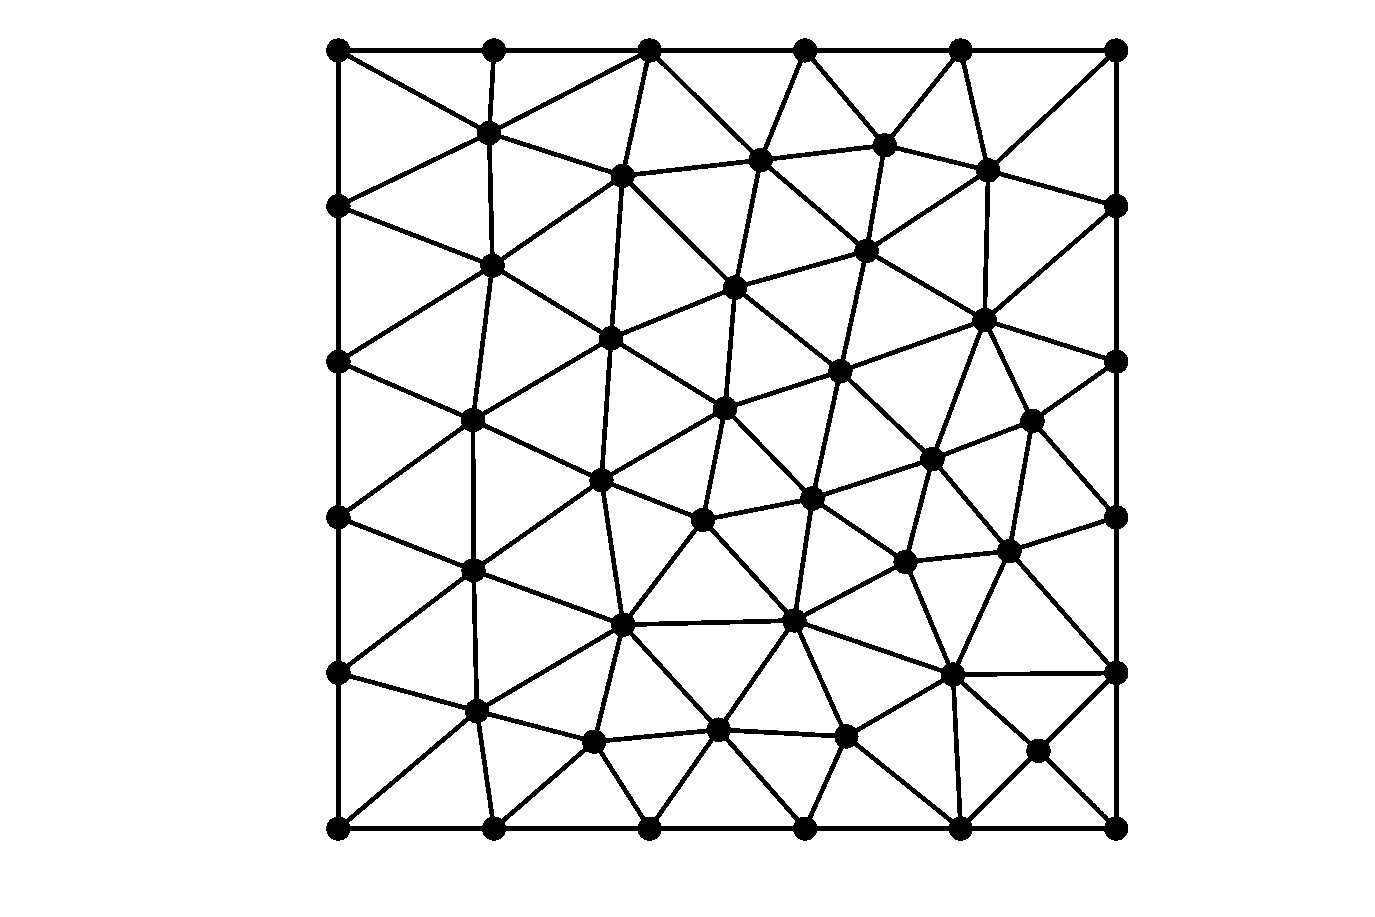
\includegraphics[scale=0.7]{figure/PHR/fenpian.png}
    \caption{分片实验无网格离散模型}\label{fenpian}
\end{figure}
为了更好的对比所提方法的计算精度,针对四阶薄板问题分别采用如下位移误差$L_2-\text{Error}$和能量误差$H_i-\text{Error}$进行分析:
\begin{equation}
\begin{split}
    &L_2-\text{Error}=\frac{\sqrt{\int_{\Omega}(w-w^h)^2d\Omega}}{\sqrt{\int_{\Omega}w^2d\Omega}}\\
    &H_i-\text{Error}=\frac{\sum_{j=0}^{i}\sqrt{\int_{\Omega}(w_{,\alpha_1\dotsb \alpha_j}-w_{,\alpha_1\dotsb \alpha_j})^2}d\Omega}{\sum_{j=0}^{i}\sqrt{\int_{\Omega}w_{,\alpha_1\dotsb \alpha_j}w_{,\alpha_1\dotsb \alpha_j}d\Omega}}
\end{split}
\end{equation}\par
针对薄板问题,三次基函数的求解计算时高斯积分法“GI”的求解域$\Omega$的积分采用13点高斯积分,边界$\Gamma$积分采用3点高斯积分;
四次基函数的求解计算时高斯积分法“GI”的求解域$\Omega$的积分采用16点高斯积分,边界$\Gamma$积分采用5点高斯积分;
再生光滑梯度积分法“RKGSI”计算时采用的积分点数和高斯积分法一致。三次和四次基函数的无网格分片试验结果如下表:
\begin{table}[H]
    \caption{\textbf{三次基函数无网格法分片实验结果}}
    \centering\label{cubic}
   \begin{tabular}{lcccc}
   \toprule
   & \multicolumn{2}{c}{二次分片实验} & \multicolumn{2}{c}{三次分片实验} \\ \cline{2-5}
   &$L_2$-Error$\quad$&$H_2$-Error&$L_2$-Error$\quad$&$H_2$-Error\\
   \midrule
   GI-Penalty&$4.27\times10^{-2}$&$3.82\times10^{-1}$&$9.54\times10^{-2}$&$5.12\times10^{-1}$\\
   GI-Nitsche&$4.09\times10^{-2}$&$3.75\times10^{-1}$&$9.50\times10^{-2}$&$5.05\times10^{-1}$\\
  RKGSI-Penalty&$4.60\times10^{-2}$&$3.86\times10^{-1}$&$1.07\times10^{-1}$&$5.40\times10^{-1}$\\
  RKGSI-Nitsche&$5.67\times10^{-14}$&$2.18\times10^{-12}$&$5.21\times10^{-14}$&$1.20\times10^{-12}$\\
  RKGSI-HR&$5.58\times10^{-15}$&$4.56\times10^{-13}$&$3.66\times10^{-15}$&$2.70\times10^{-13}$\\
   \bottomrule
   \end{tabular}
   \end{table}
\begin{table}[H]
    \caption{\textbf{四次基函数无网格法分片实验结果}}
    \centering\label{quartic}
   \begin{tabular}{lcccc}
   \toprule
   & \multicolumn{2}{c}{三次分片实验} & \multicolumn{2}{c}{四次分片实验} \\ \cline{2-5}
   &$L_2$-Error$\quad$&$H_1$-Error&$L_2$-Error$\quad$&$H_1$-Error\\
   \midrule
   GI-Penalty&$1.08\times10^{-1}$&$5.44\times10^{-1}$&$1.84\times10^{-1}$&$6.32\times10^{-1}$\\
   GI-Nitsche&$1.07\times10^{-1}$&$5.45\times10^{-1}$&$1.84\times10^{-1}$&$6.34\times10^{-1}$\\
  RKGSI-Penalty&$1.06\times10^{-1}$&$5.40\times10^{-1}$&$1.84\times10^{-1}$&$6.26\times10^{-1}$\\
  RKGSI-Nitsche&$2.82\times10^{-13}$&$4.99\times10^{-12}$&$3.03\times10^{-13}$&$3.33\times10^{-12}$\\
  RKGSI-HR&$1.68\times10^{-14}$&$2.33\times10^{-12}$&$4.40\times10^{-14}$&$1.57\times10^{-12}$\\
\bottomrule
\end{tabular}
\end{table}\par
表(\ref{cubic})和表(\ref{quartic})分别表示具有三次、四次基函数无网格法的薄板分片试验结果,从表中可以明显的看出,由于缺乏变分一致性
传统高斯积分法“GI-Penalty”、“GI-Nitsche”和罚函数法“RKGSI-Penalty”都无法通过分片试验。只有满足变分一致性的再生光滑梯度积分法的“RKGSI-Nitsche”法和
本章提出的Hellinger-Ressiner变分原理的本质边界条件施加方案“RKGSI-HR”法可以通过分片试验,满足积分约束条件。
\subsection{简支方板问题}
如图(\ref{rectangular})所示,一简支方板的中性面区域为$\Omega=(0,1)\otimes(0,1)$,此时$\Omega$的长为$a=1$宽为$b=1$,材料系数分别为弯曲刚度$\bar{D}=1$、$\nu=0.3$。板面内分布如图所示纵向荷载:
\begin{equation}
\begin{split}
    \bar q=-\bar D(\frac{\pi^2}{a^2}+\frac{\pi^2}{b^2})\sin(\frac{\pi}{a}x)\sin(\frac{\pi}{b}y)
\end{split}
\end{equation}
该简支方板问题的精确解为:
\begin{equation}
\begin{split}
    w=-\sin(\frac{\pi}{a}x)\sin(\frac{\pi}{b}y)
\end{split}
\end{equation}
\newpage
\begin{figure}[H]
\centering
    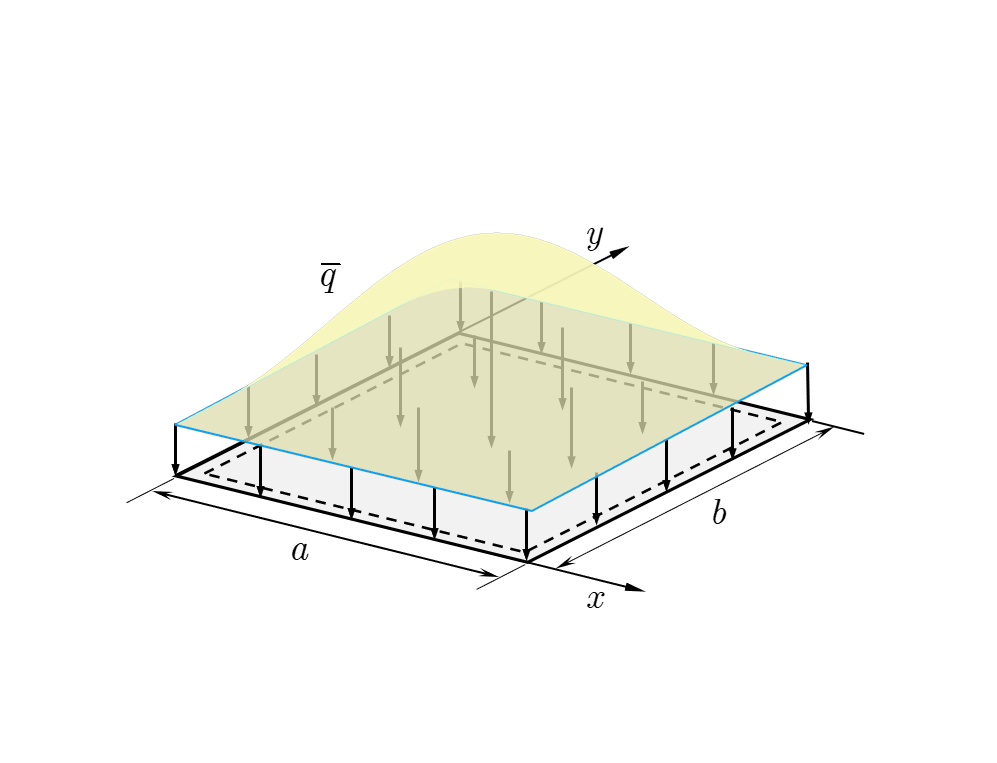
\includegraphics[scale=0.7]{figure/PHR/R/rectangular.png}
    \caption{简支方板问题模型}\label{rectangular}
\end{figure}
如图所示(\ref{rectangularmsh}),简支方板求解域采用均布的$11\times 11$、$21\times 21$、$41\times 41$、$81\times 81$的四个疏密不同的节点进行离散。
此时对于采用三次基函数的简支方板问题其相对影响域取为3.5,采用四次基函数时其相对影响域则取为4.5。\par
\begin{figure}[H]
\centering
      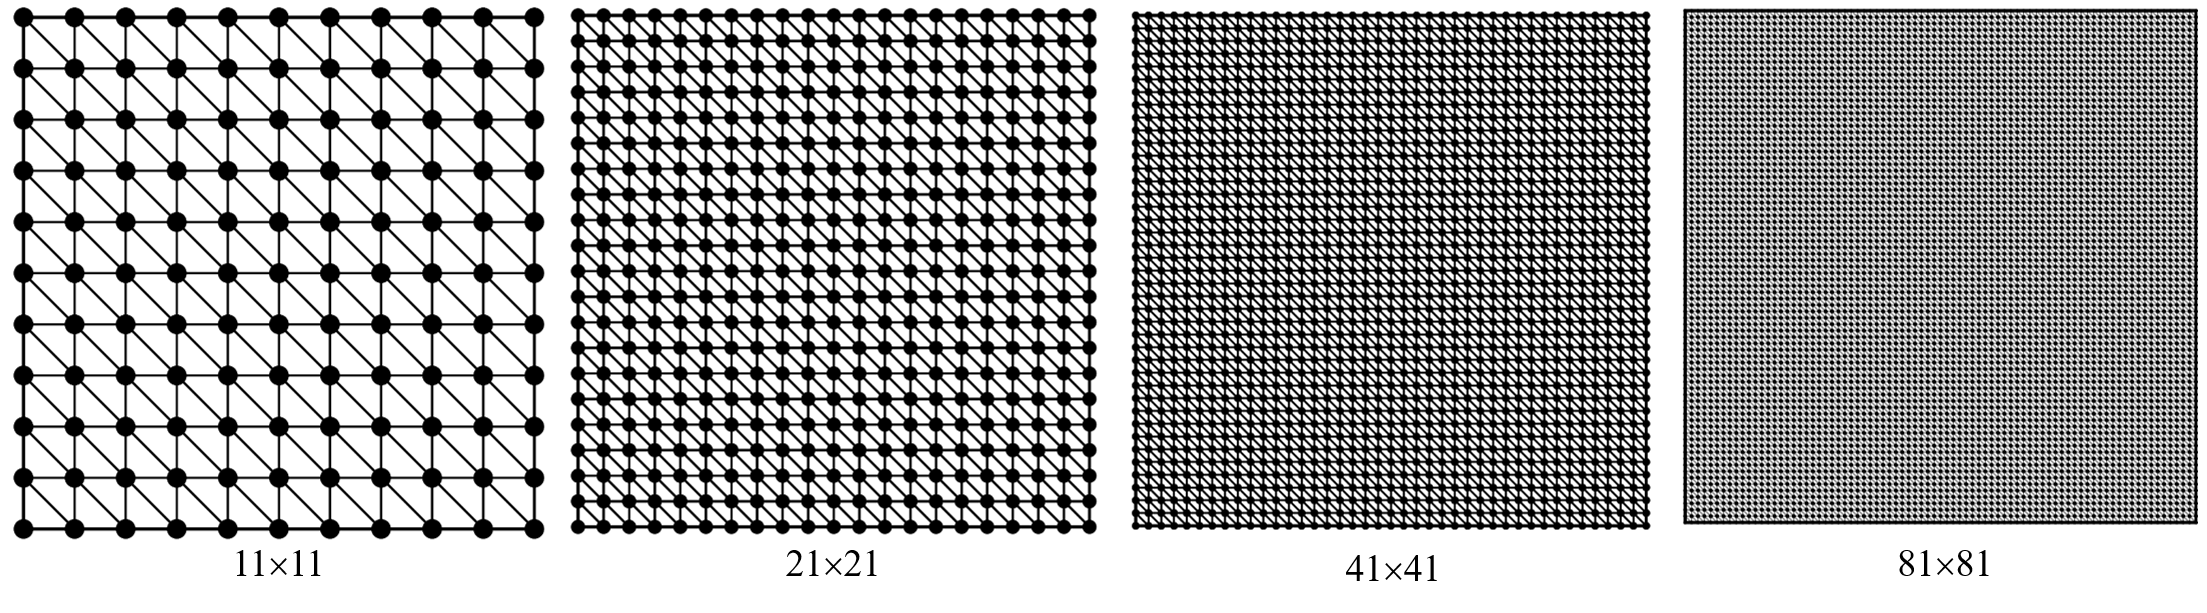
\includegraphics[scale=0.4]{figure/PHR/R/rectangularmsh.png}
    \caption{简支方板问题节点离散}\label{rectangularmsh}
\end{figure}
\newpage
 图(\ref{RCLH})、图(\ref{RQLH})分别为简支方板问题在三次基函数和四次基函数时的位移误差和能量误差对比图。从图中可以明显看出即使采用高阶高斯积分法“GI”如三次基函数的13点高斯积分法和四次基函数的16点高斯积分,
计算精度都低于再生光滑梯度法“RKGSI”,并且和同样不满足变分一致性的罚函数法一样都无法达到理论误差收敛率。而“RKGSI-Nitsche”和“RKGSI-HR”法不管是在三次基函数还是四次基函数时都达到了误差收敛率。
图(\ref{RCcputime})、图(\ref{RQcputime})是简支方板问题在三次基函数和四次基函数时分别计算节点数和与使用“GI”和“RKGSI”不同数值积分方法时的效率图。从整体来看采用“RKGSI”时的计算效率在三次基函数和四次基函数时都明显高于“GI”。  
\begin{figure}[H]
    \centering
    \begin{subcaptiongroup}
    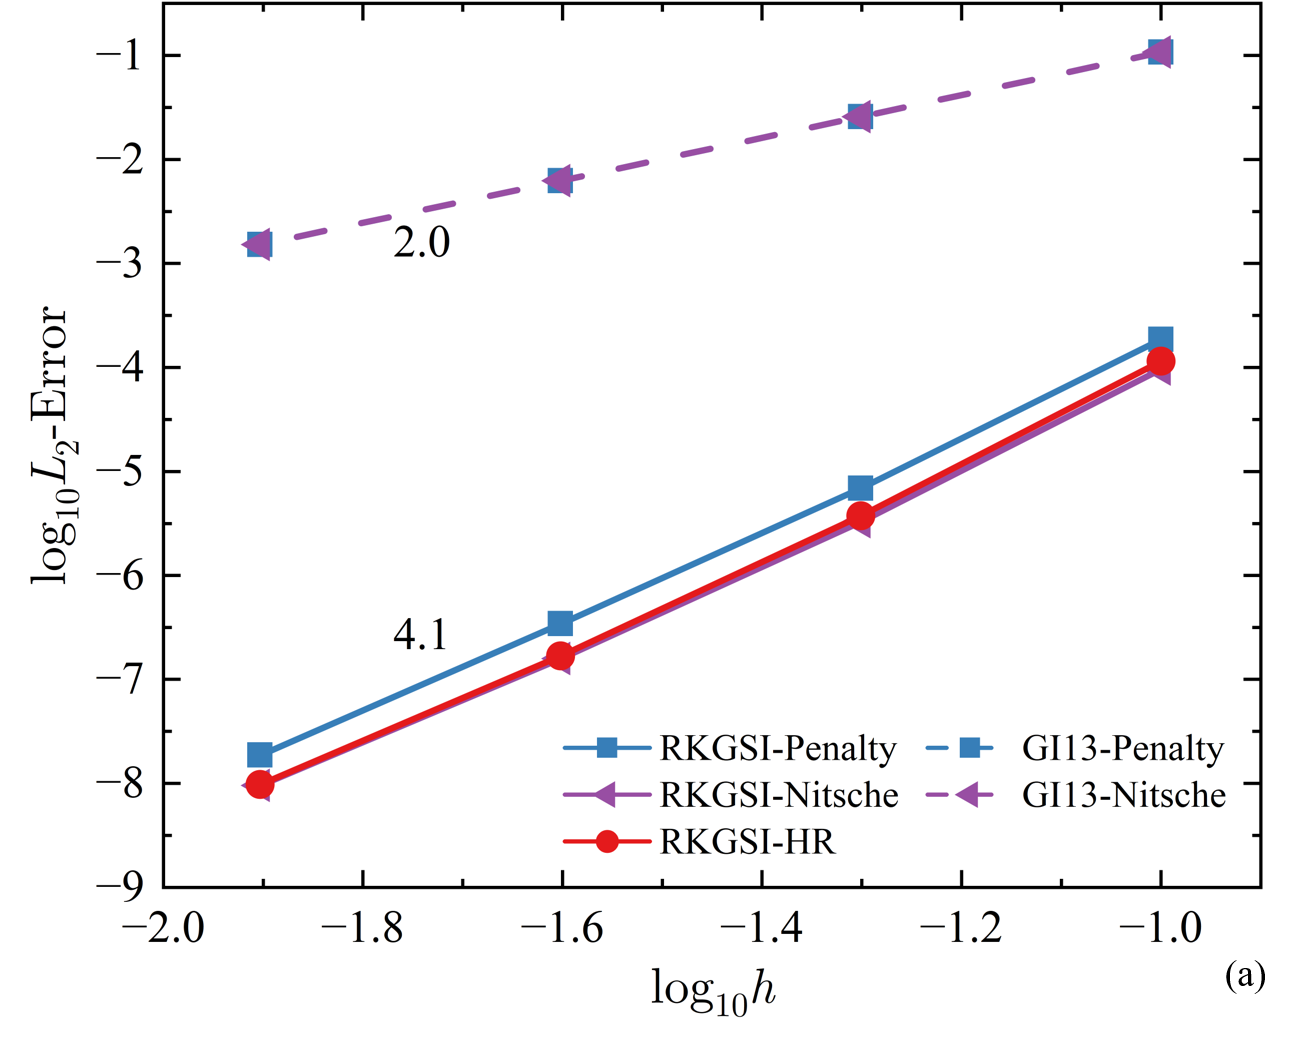
\includegraphics[width=0.49\textwidth]{figure/PHR/R/CL2.png}
    \phantomcaption\label{CL2}
    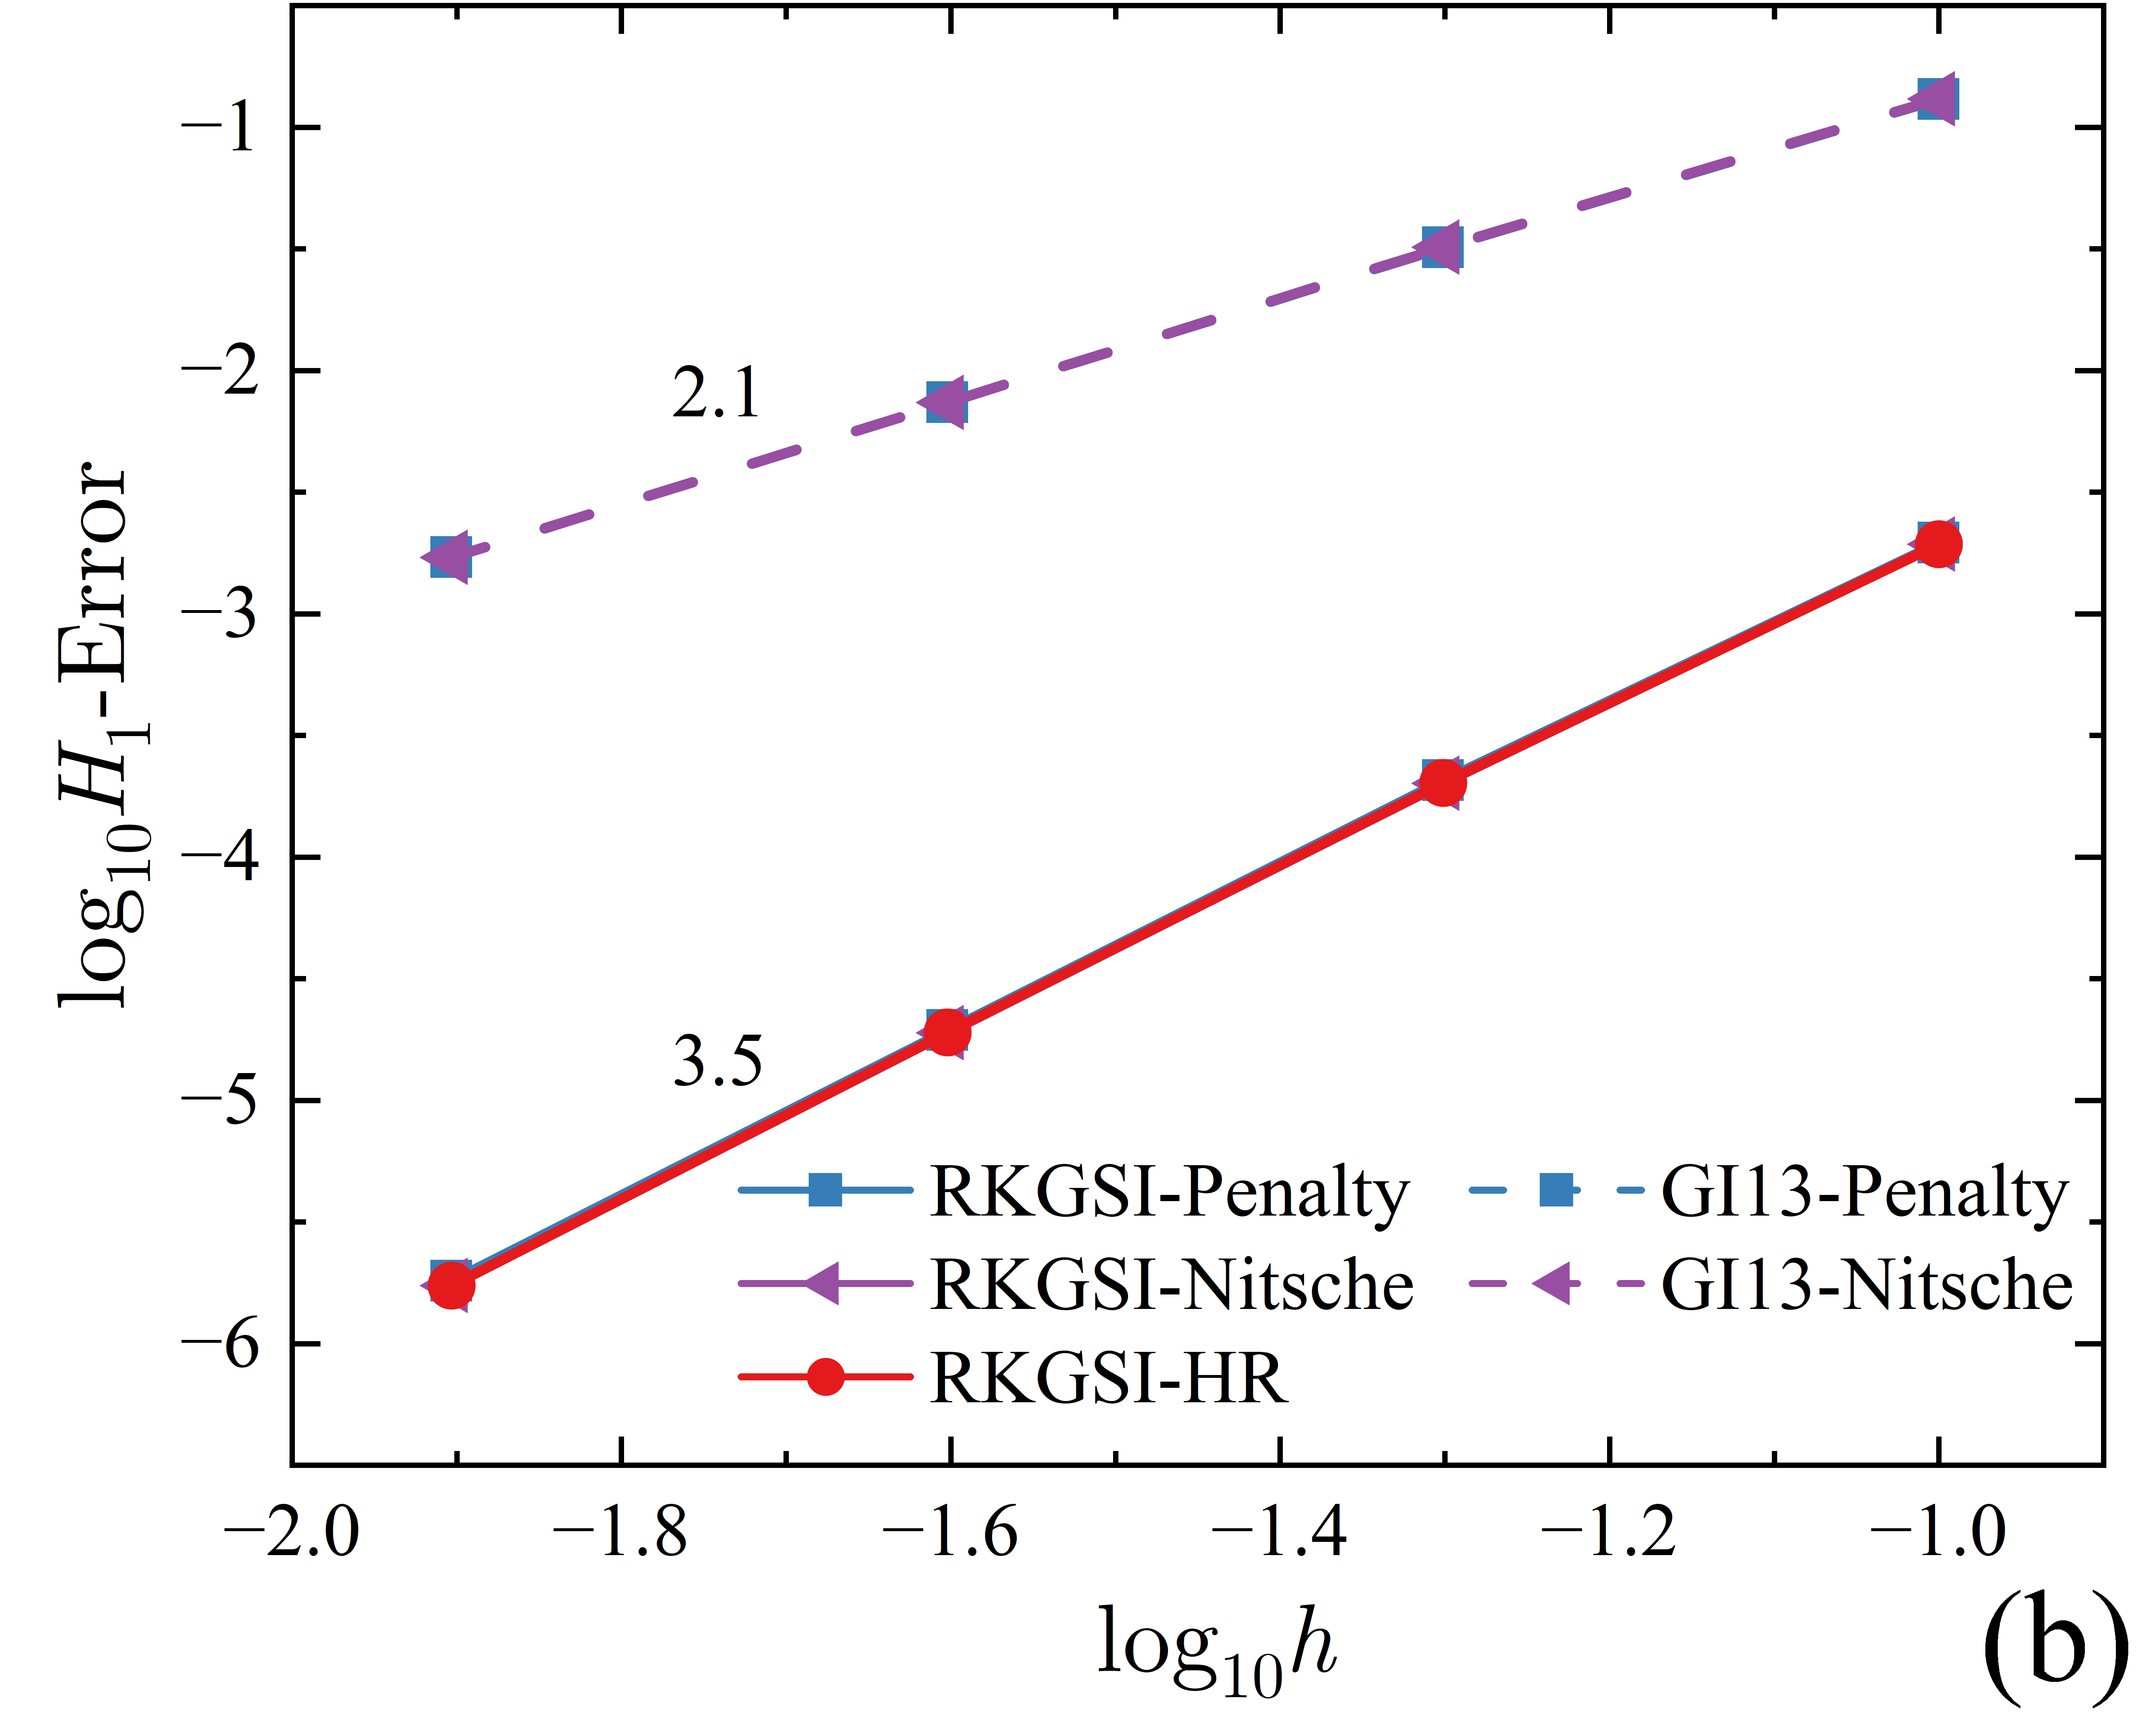
\includegraphics[width=0.49\textwidth]{figure/PHR/R/CH1.png}
    \phantomcaption\label{CH1}
    \end{subcaptiongroup}
    \begin{subcaptiongroup}
    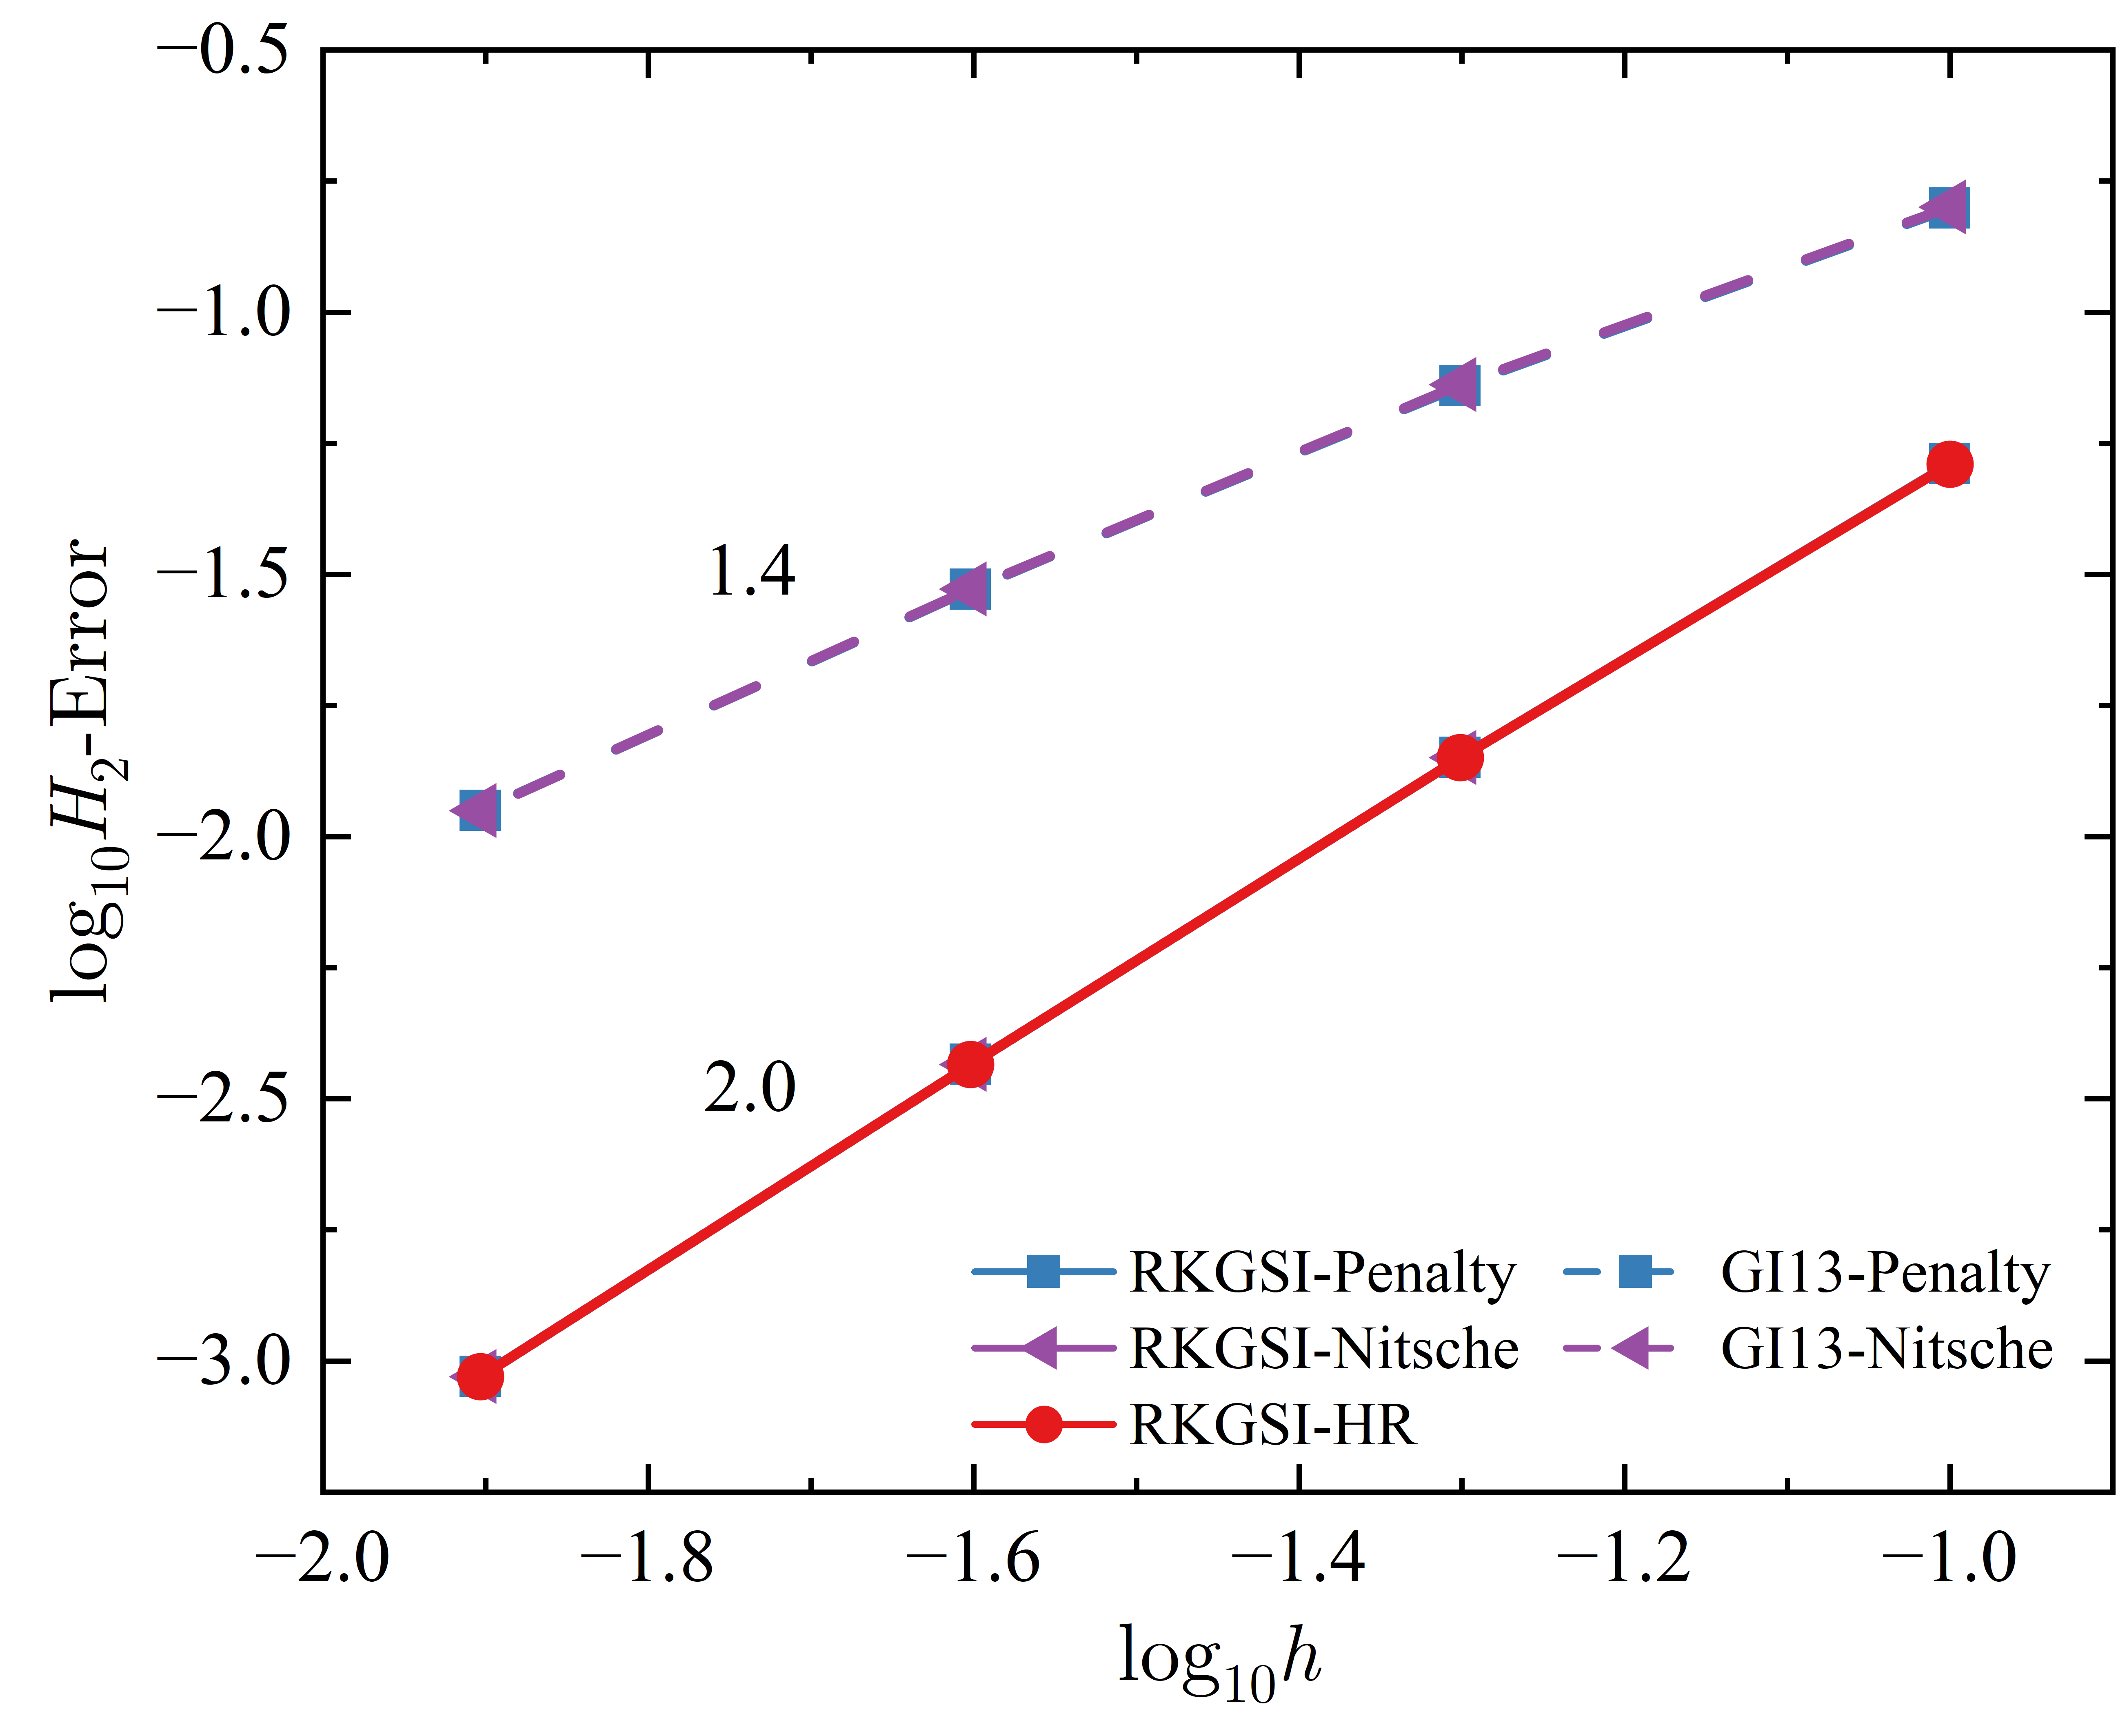
\includegraphics[width=0.49\textwidth]{figure/PHR/R/CH2.png}
    \phantomcaption\label{CH2}
    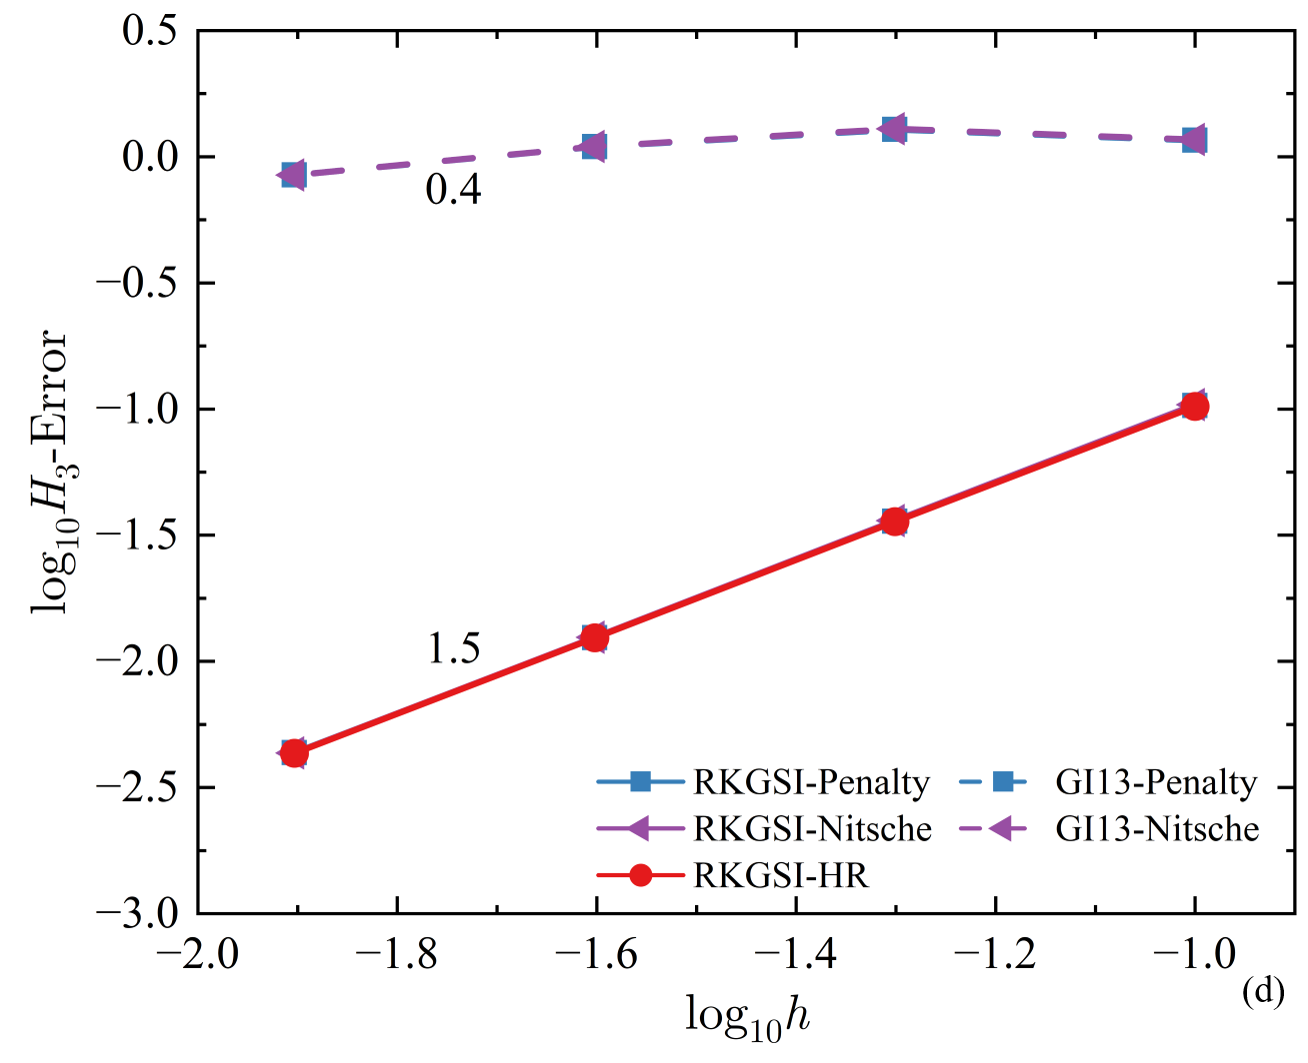
\includegraphics[width=0.49\textwidth]{figure/PHR/R/CH3.png}
    \phantomcaption\label{CH3}
    \end{subcaptiongroup}
\caption{简支方板问题三次基函数误差对比:\subref{CL2} $L_2$误差;\subref{CH1} $H_1$误差;\subref{CH2}$H_2$误差;\subref{CH3} $H_3$误差}
\label{RCLH}
\end{figure}
\newpage
\begin{figure}[H]
    \centering
    \begin{subcaptiongroup}
    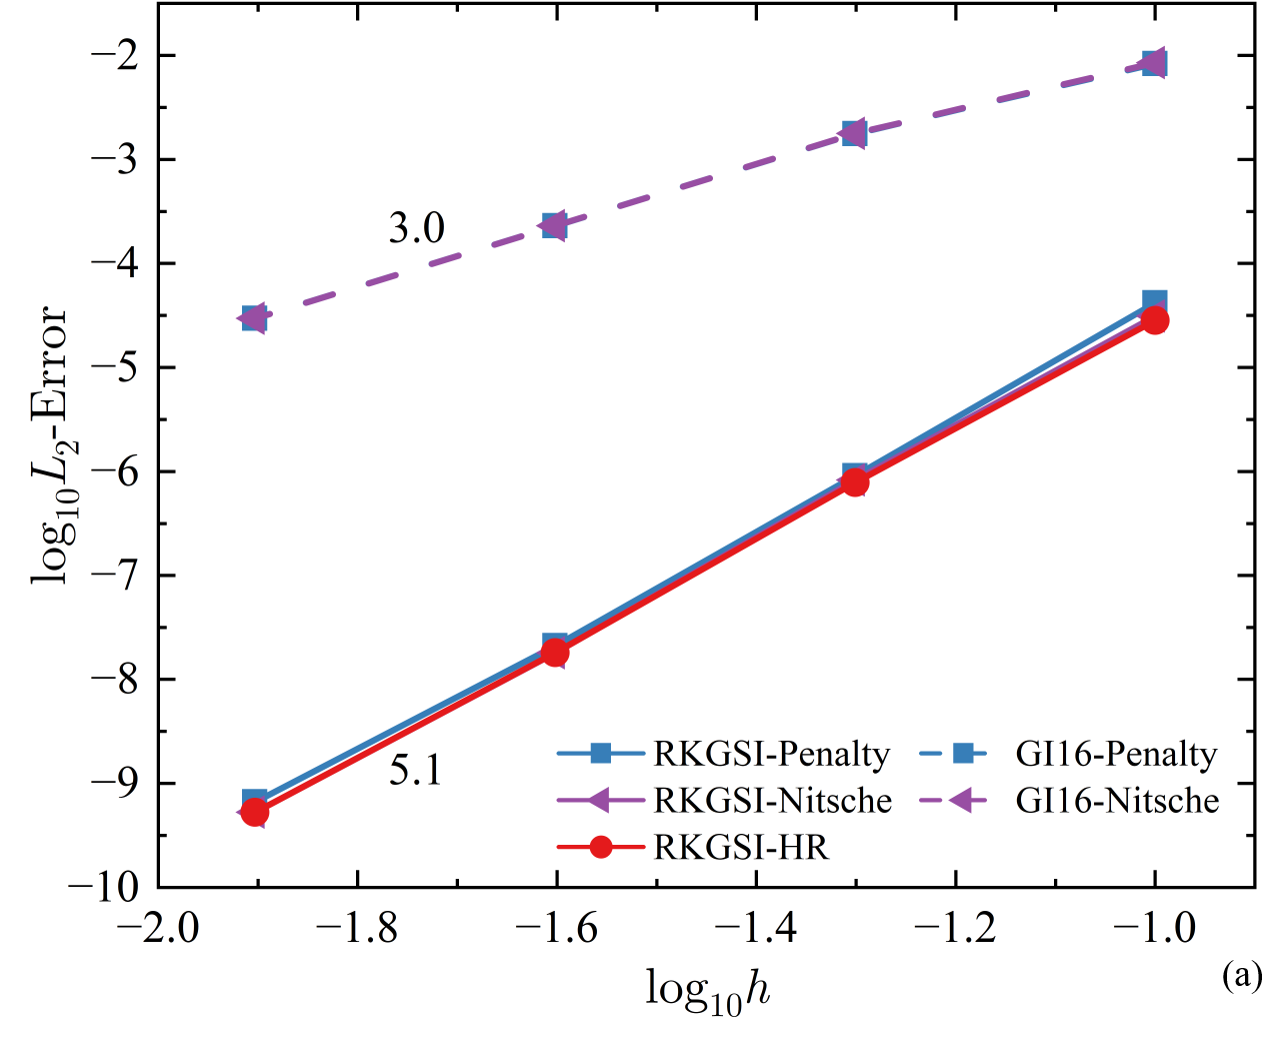
\includegraphics[width=0.49\textwidth]{figure/PHR/R/QL2.png}
    \phantomcaption\label{QL2}
    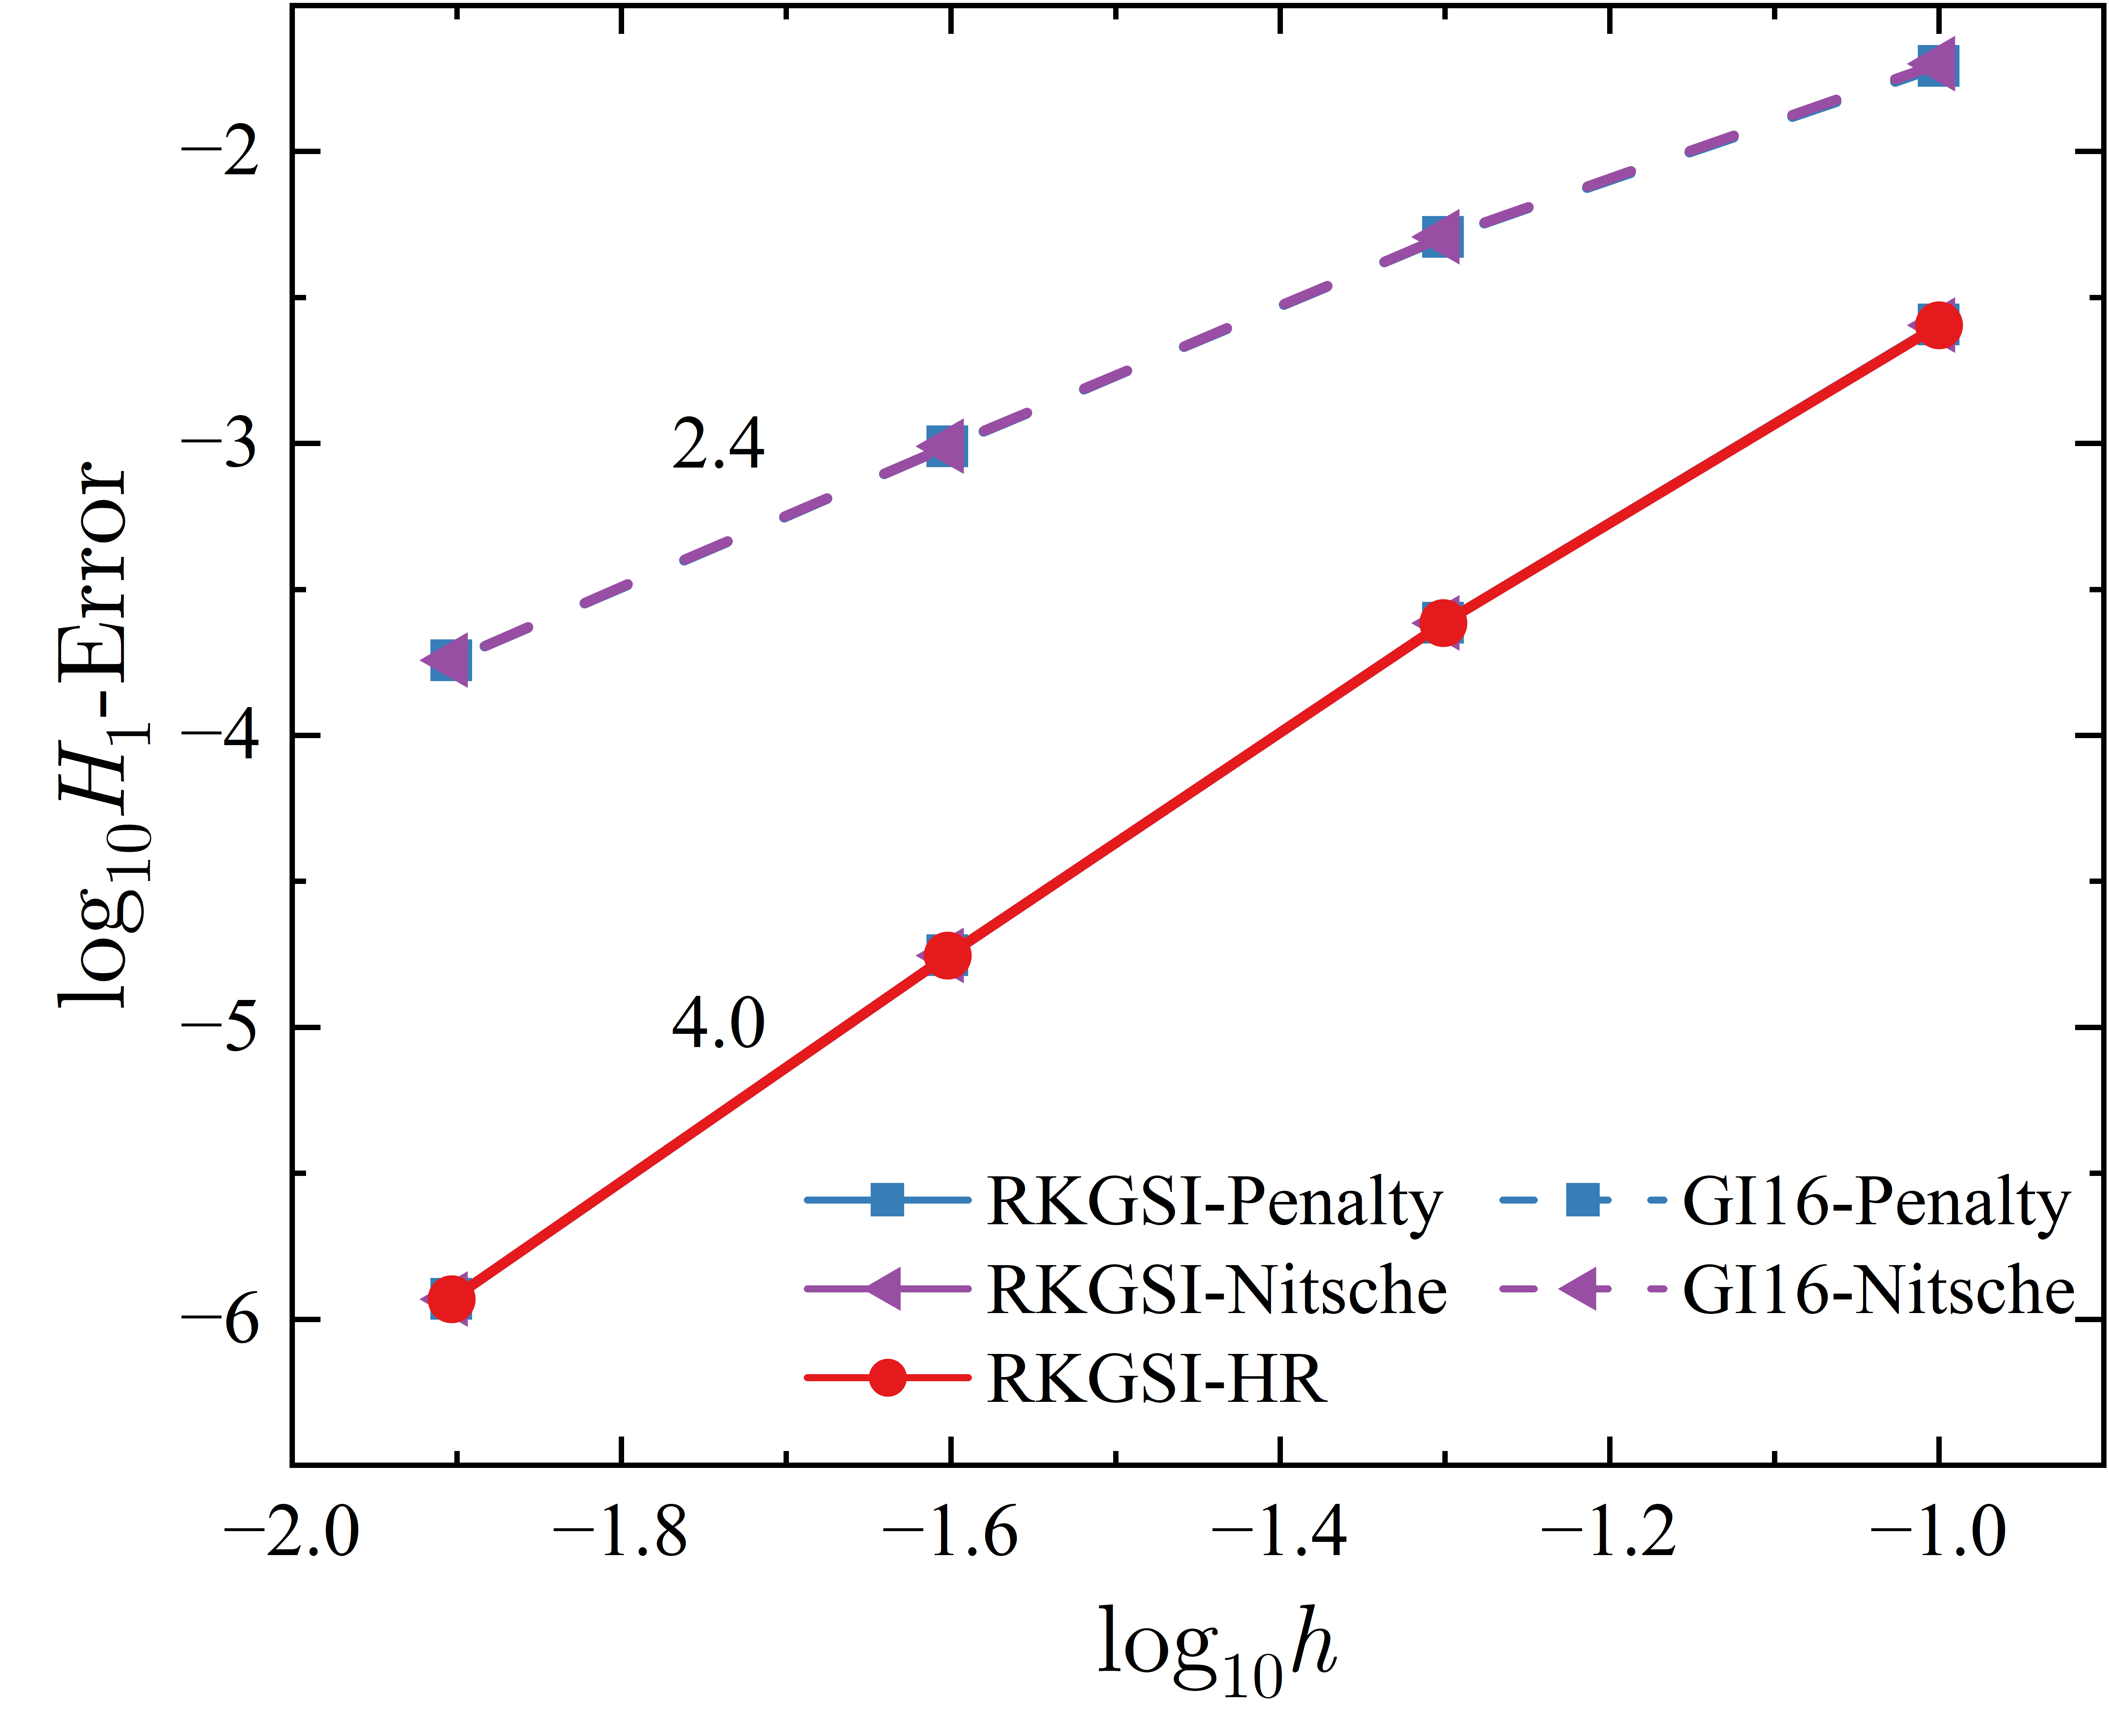
\includegraphics[width=0.49\textwidth]{figure/PHR/R/QH1.png}
    \phantomcaption\label{QH1}
    \end{subcaptiongroup}
    \begin{subcaptiongroup}
    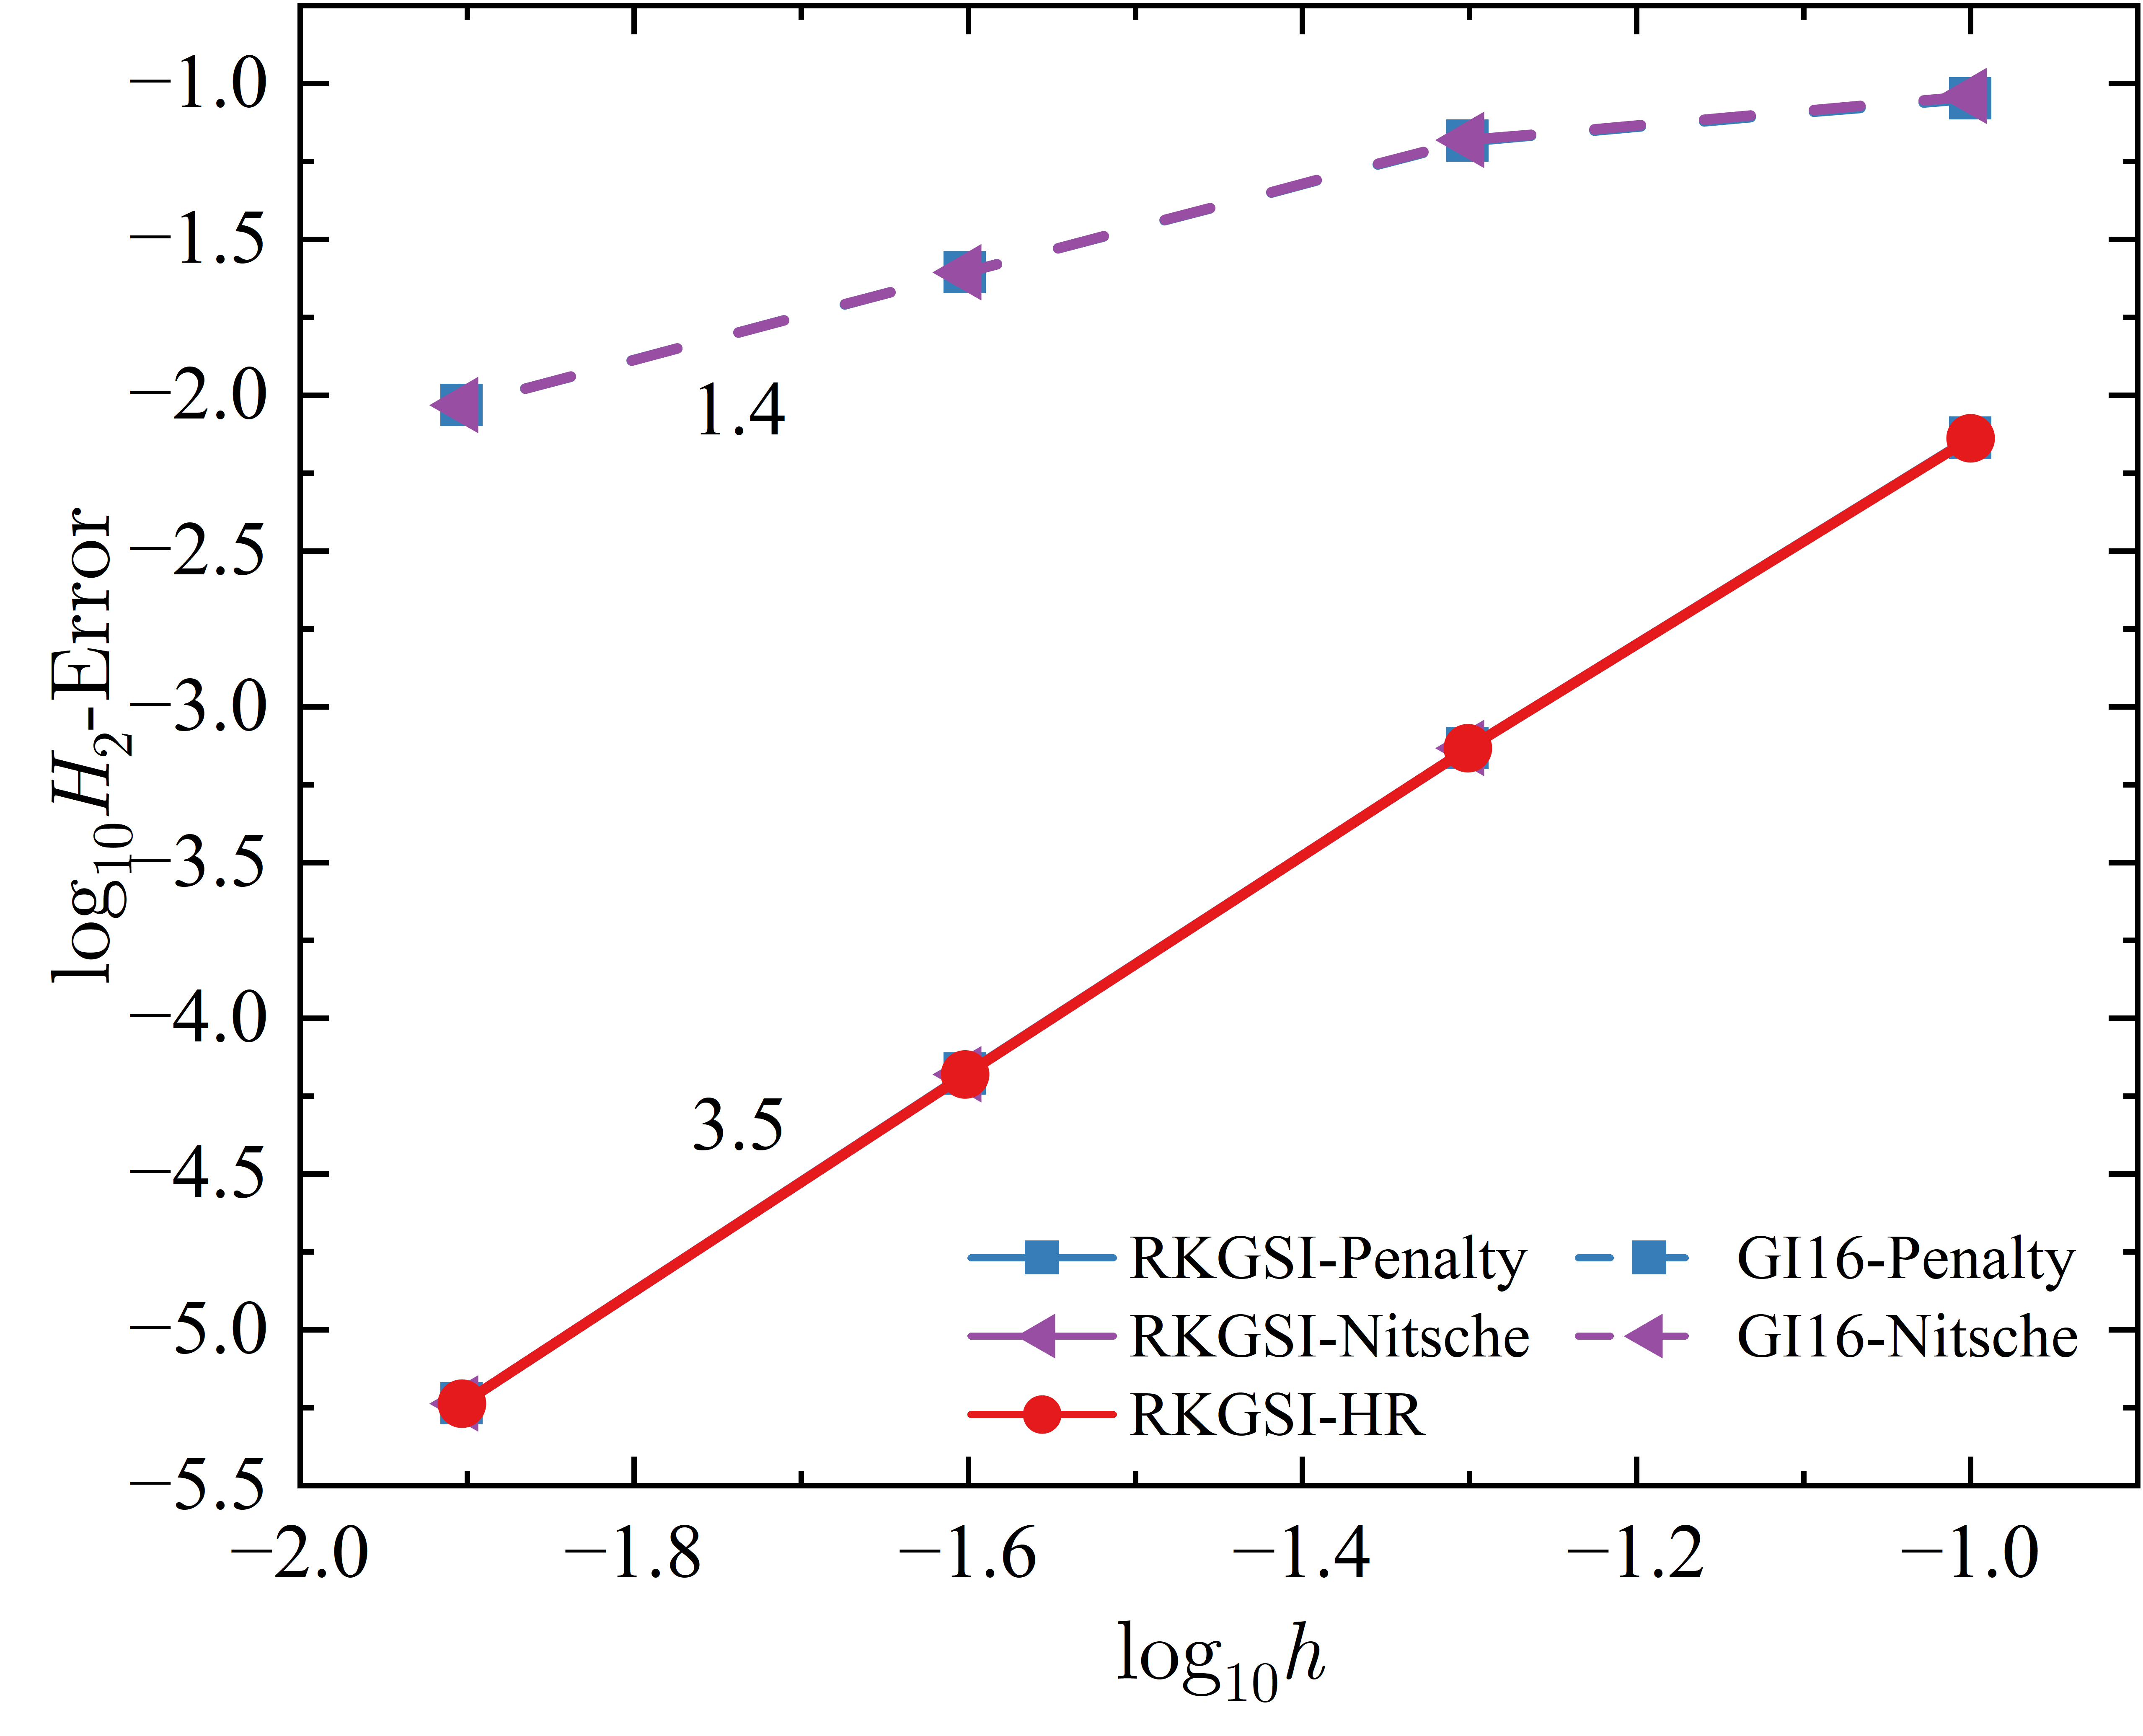
\includegraphics[width=0.49\textwidth]{figure/PHR/R/QH2.png}
    \phantomcaption\label{QH2}
    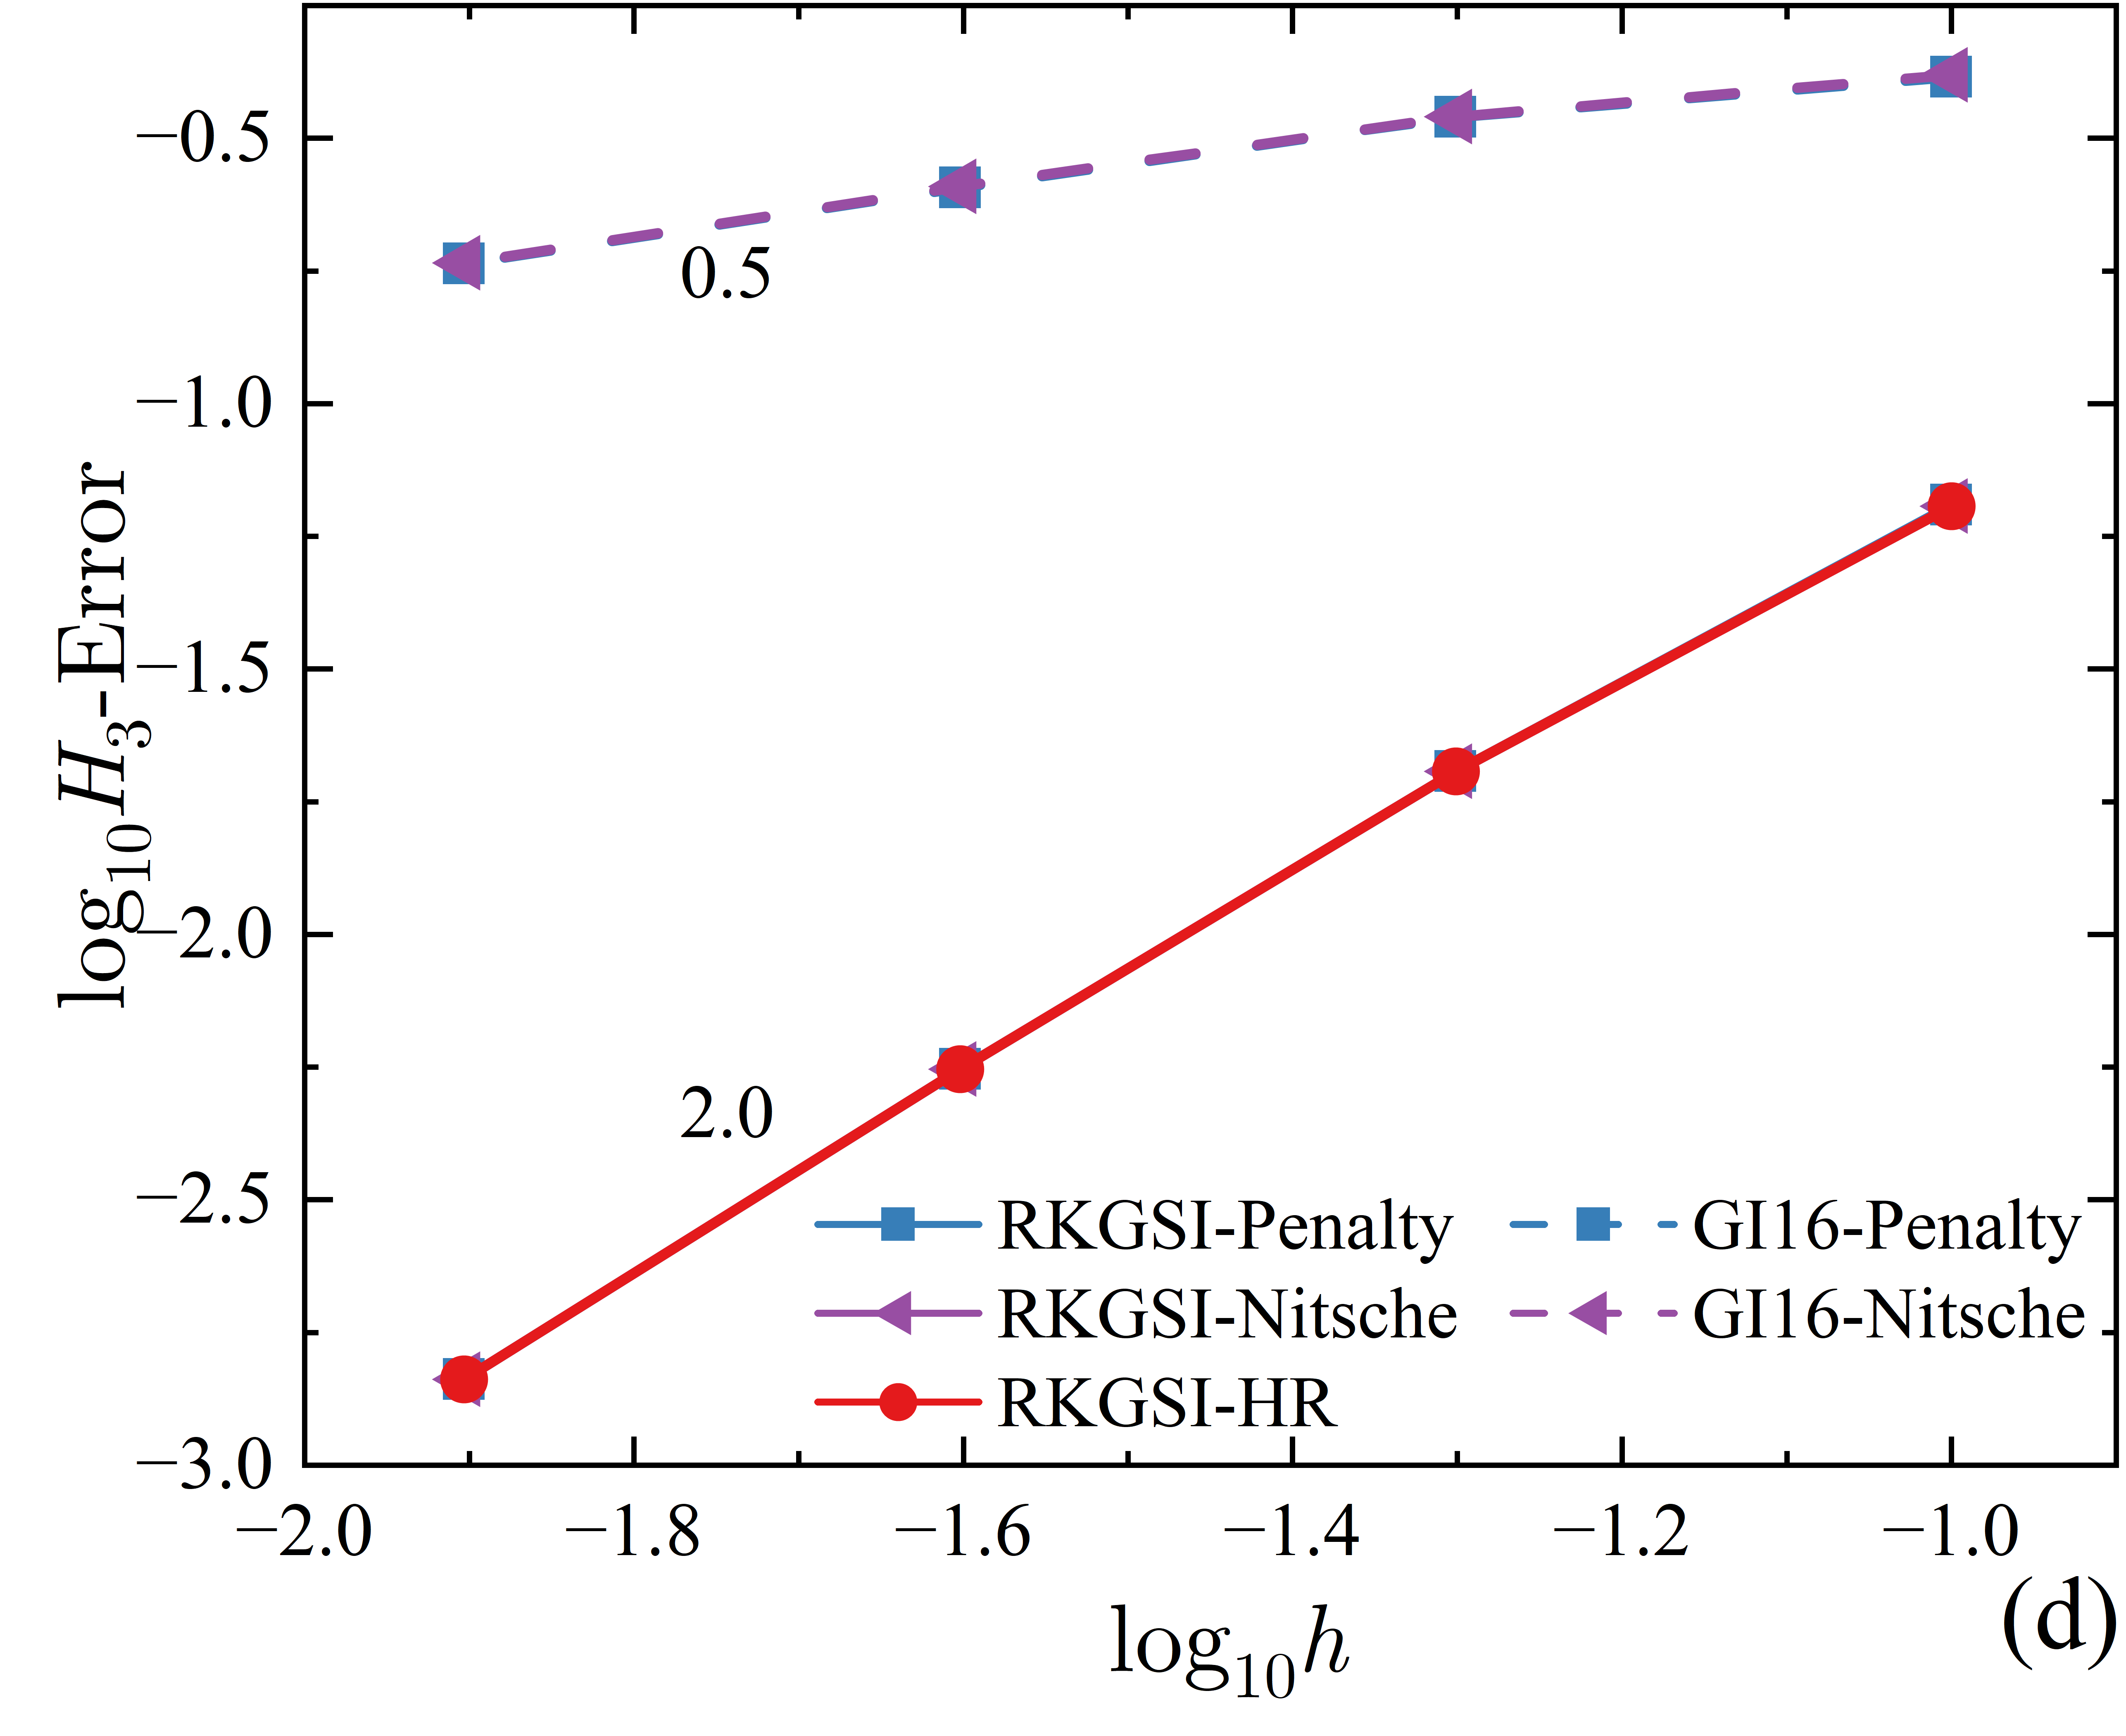
\includegraphics[width=0.49\textwidth]{figure/PHR/R/QH3.png}
    \phantomcaption\label{QH3}
    \end{subcaptiongroup}
\caption{简支方板问题四次基函数误差对比:\subref{QL2} $L_2$误差;\subref{QH1} $H_1$误差;\subref{QH2}$H_2$误差;\subref{QH3} $H_3$误差}
\label{RQLH}
\end{figure}
\begin{figure}[H]
    \centering
    \begin{subcaptiongroup}
    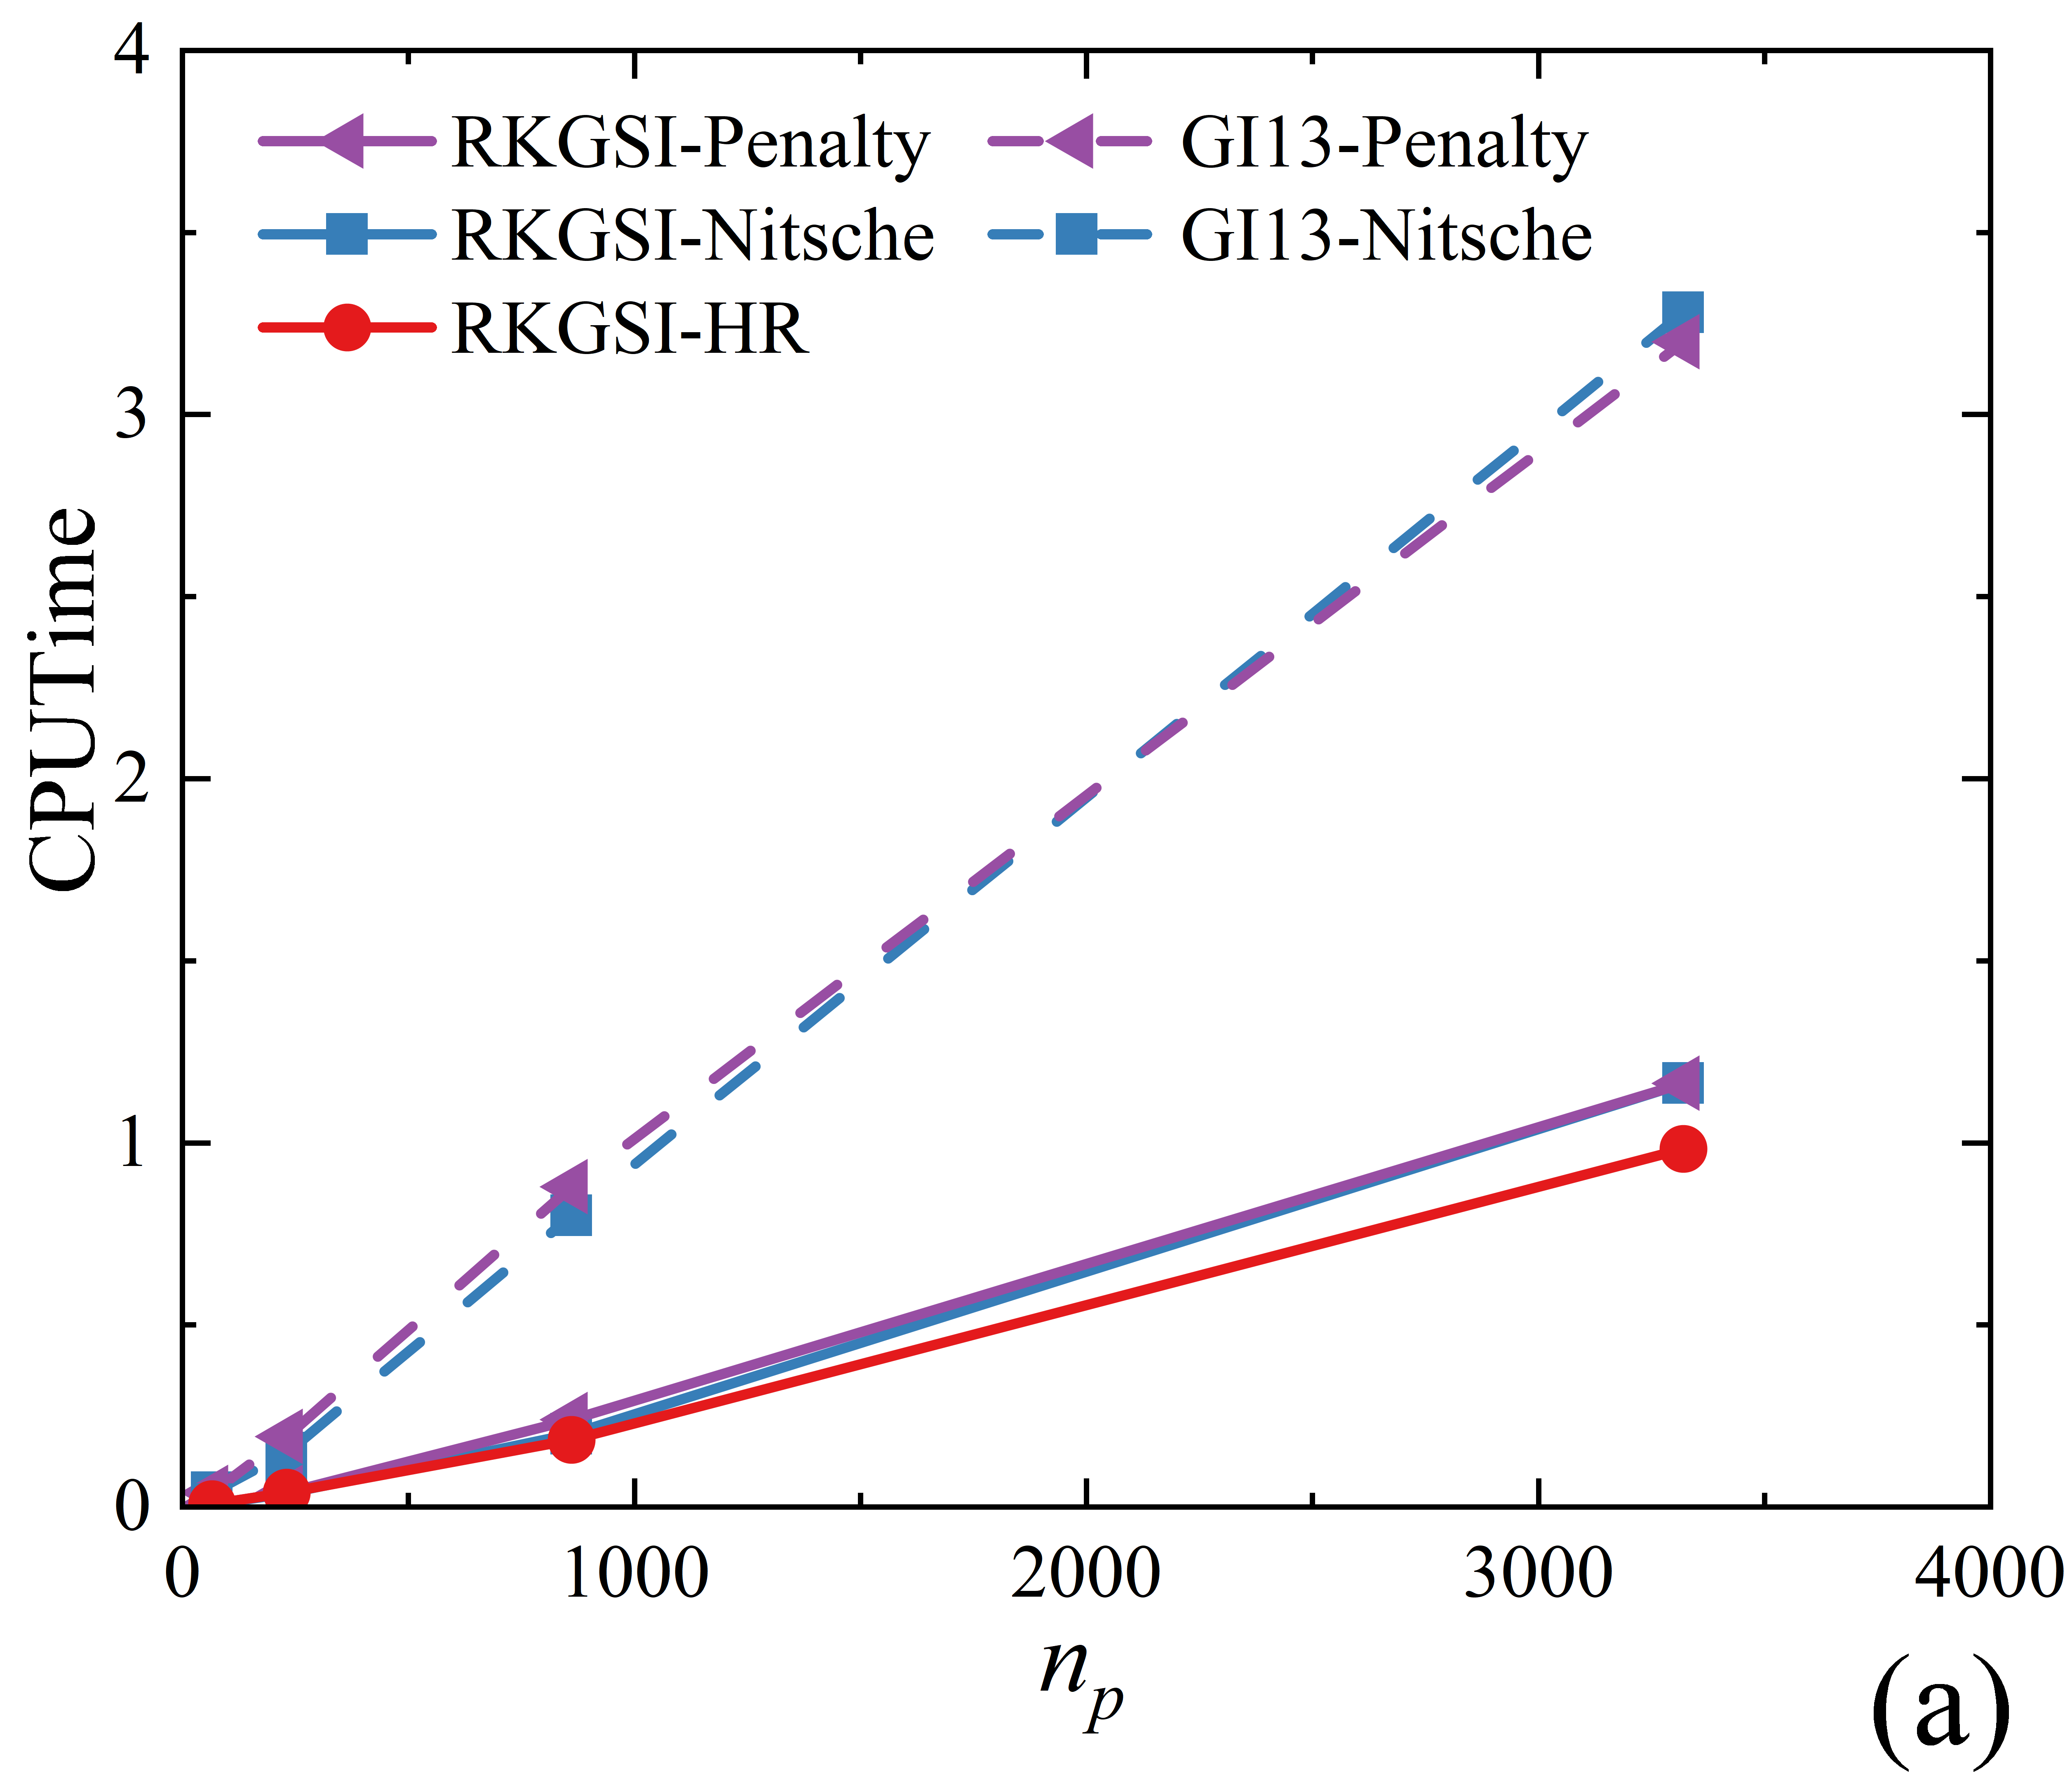
\includegraphics[width=0.49\textwidth]{figure/PHR/R/Ccputime.png}
    \phantomcaption\label{Ccputime}
    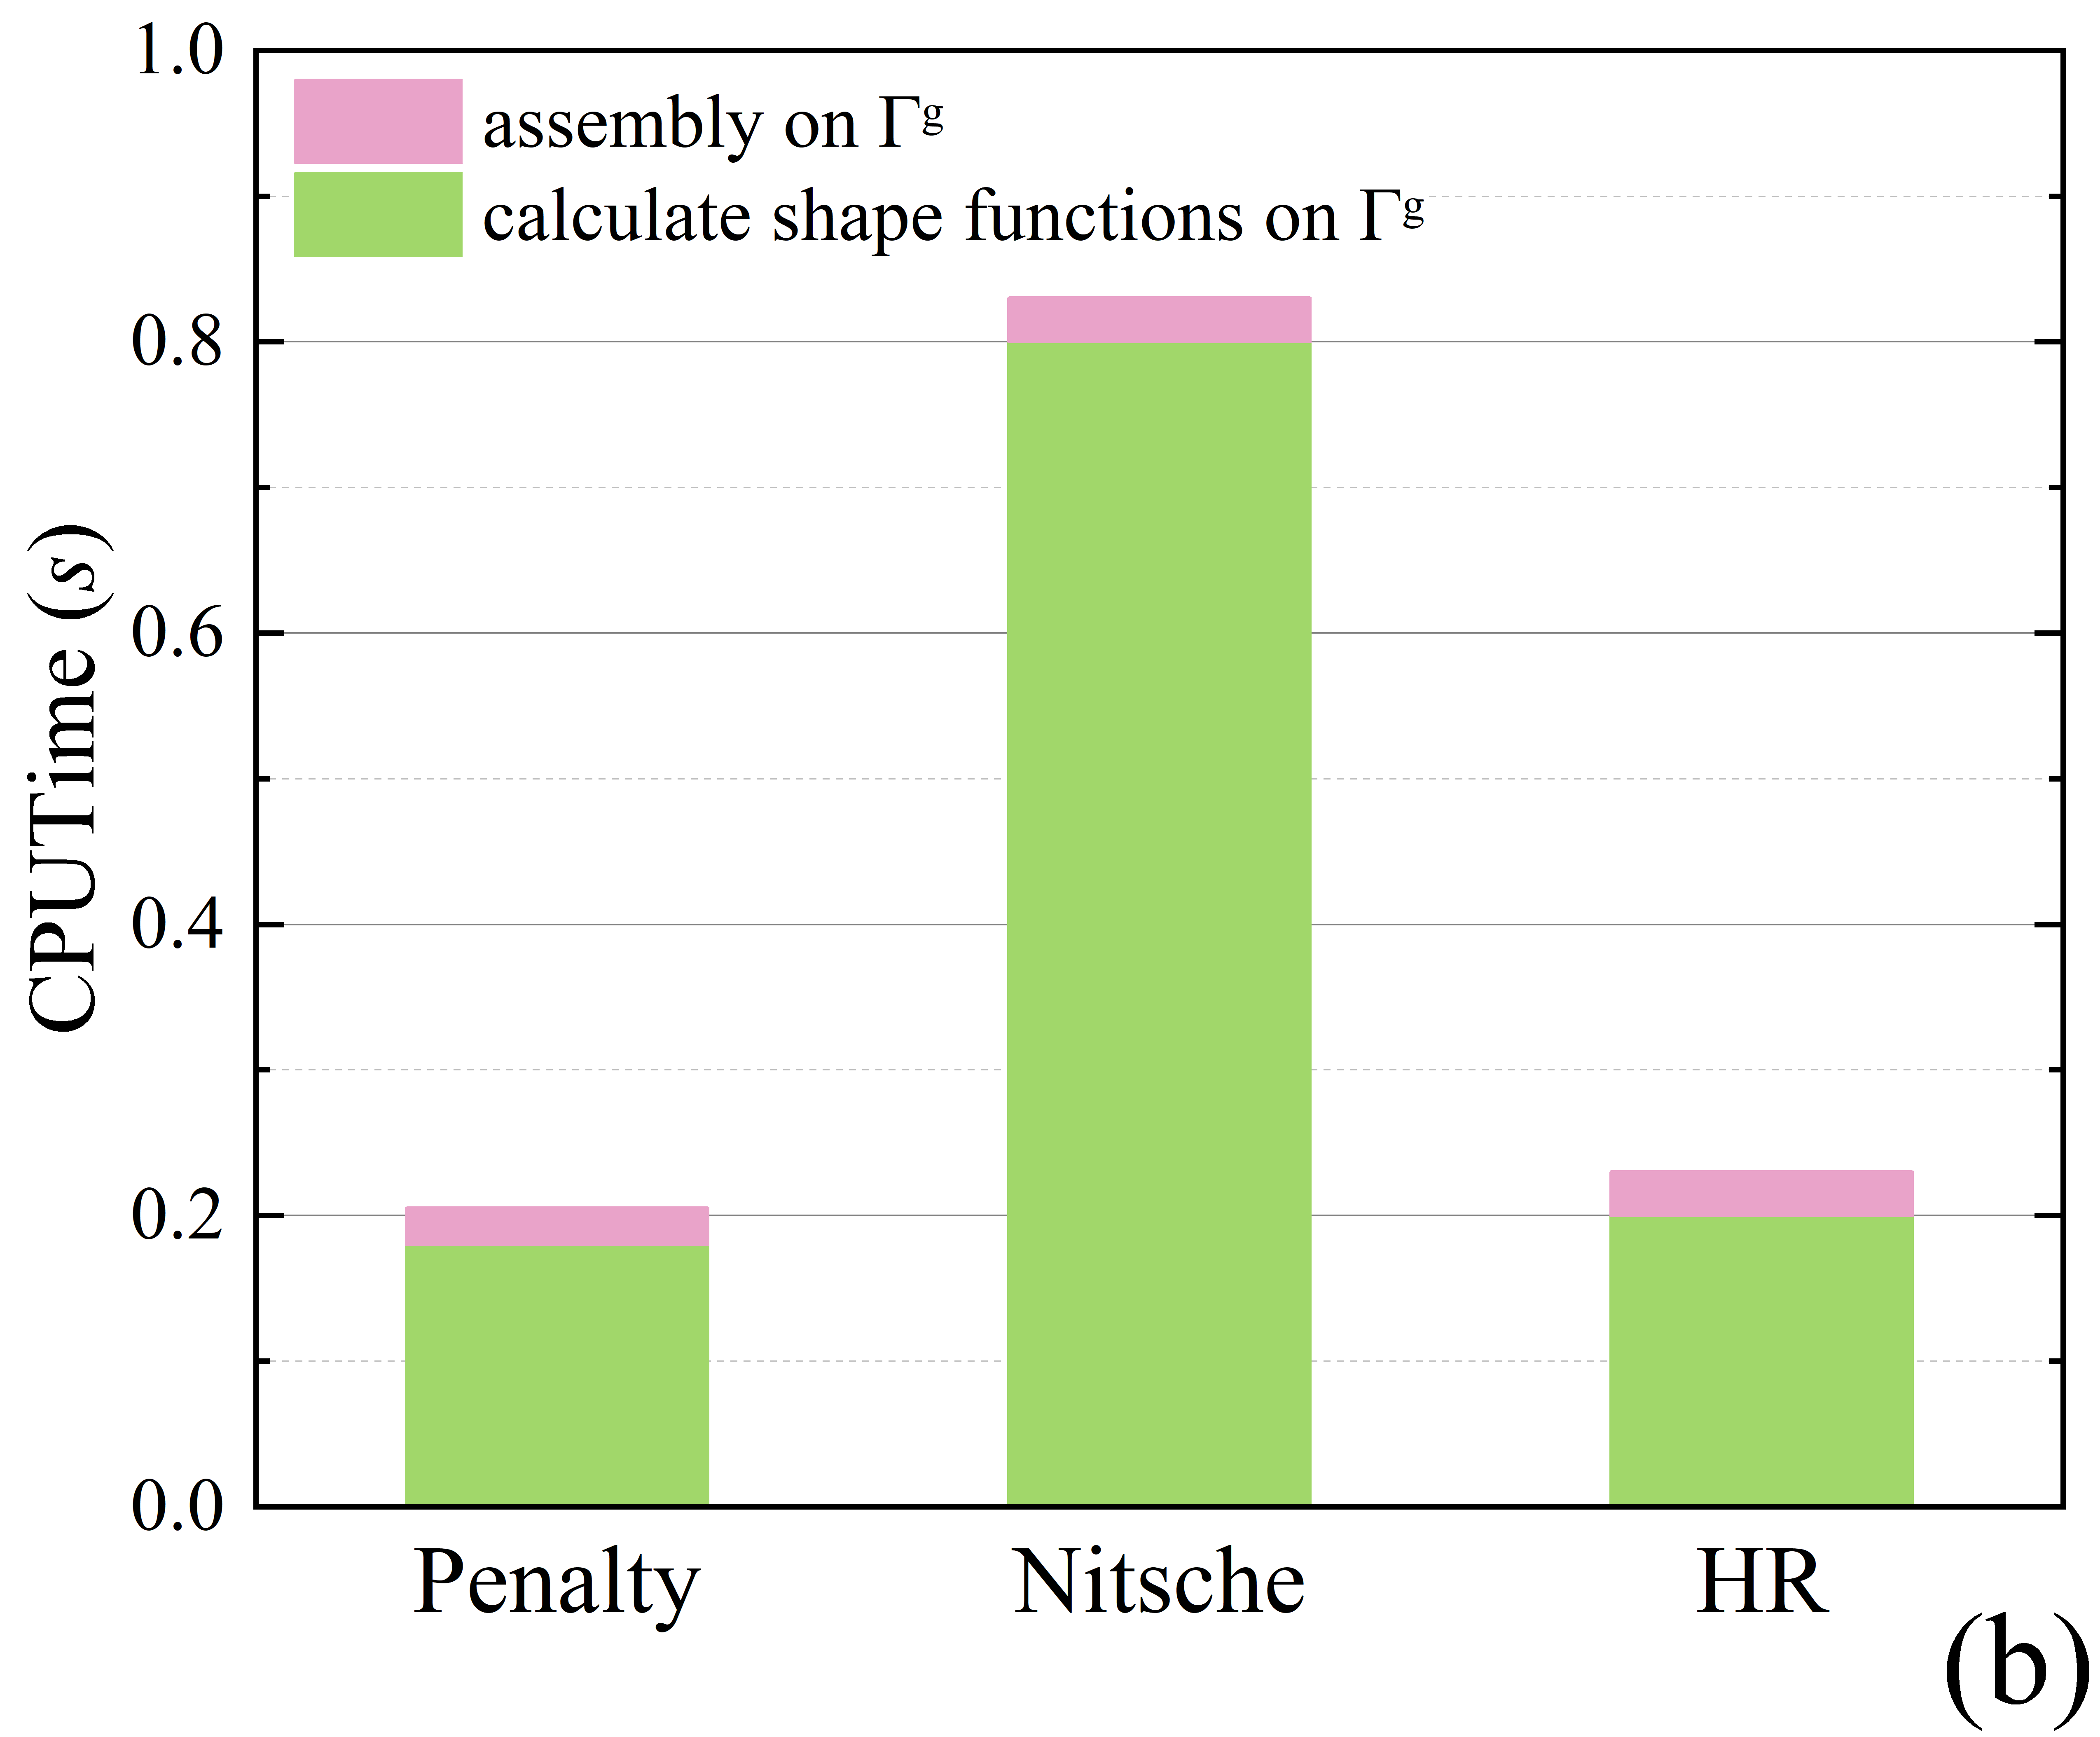
\includegraphics[width=0.49\textwidth]{figure/PHR/R/Cefficiency.png}
    \phantomcaption\label{Cefficiency}
    \end{subcaptiongroup}
\caption{简支方板问题三次基函数效率对比:\subref{Ccputime}计算时间与节点数的关系;\subref{Cefficiency}本质边界条件施加效率分析}
\label{RCcputime}
\end{figure}
\newpage
\begin{figure}[H]
    \centering
    \begin{subcaptiongroup}
    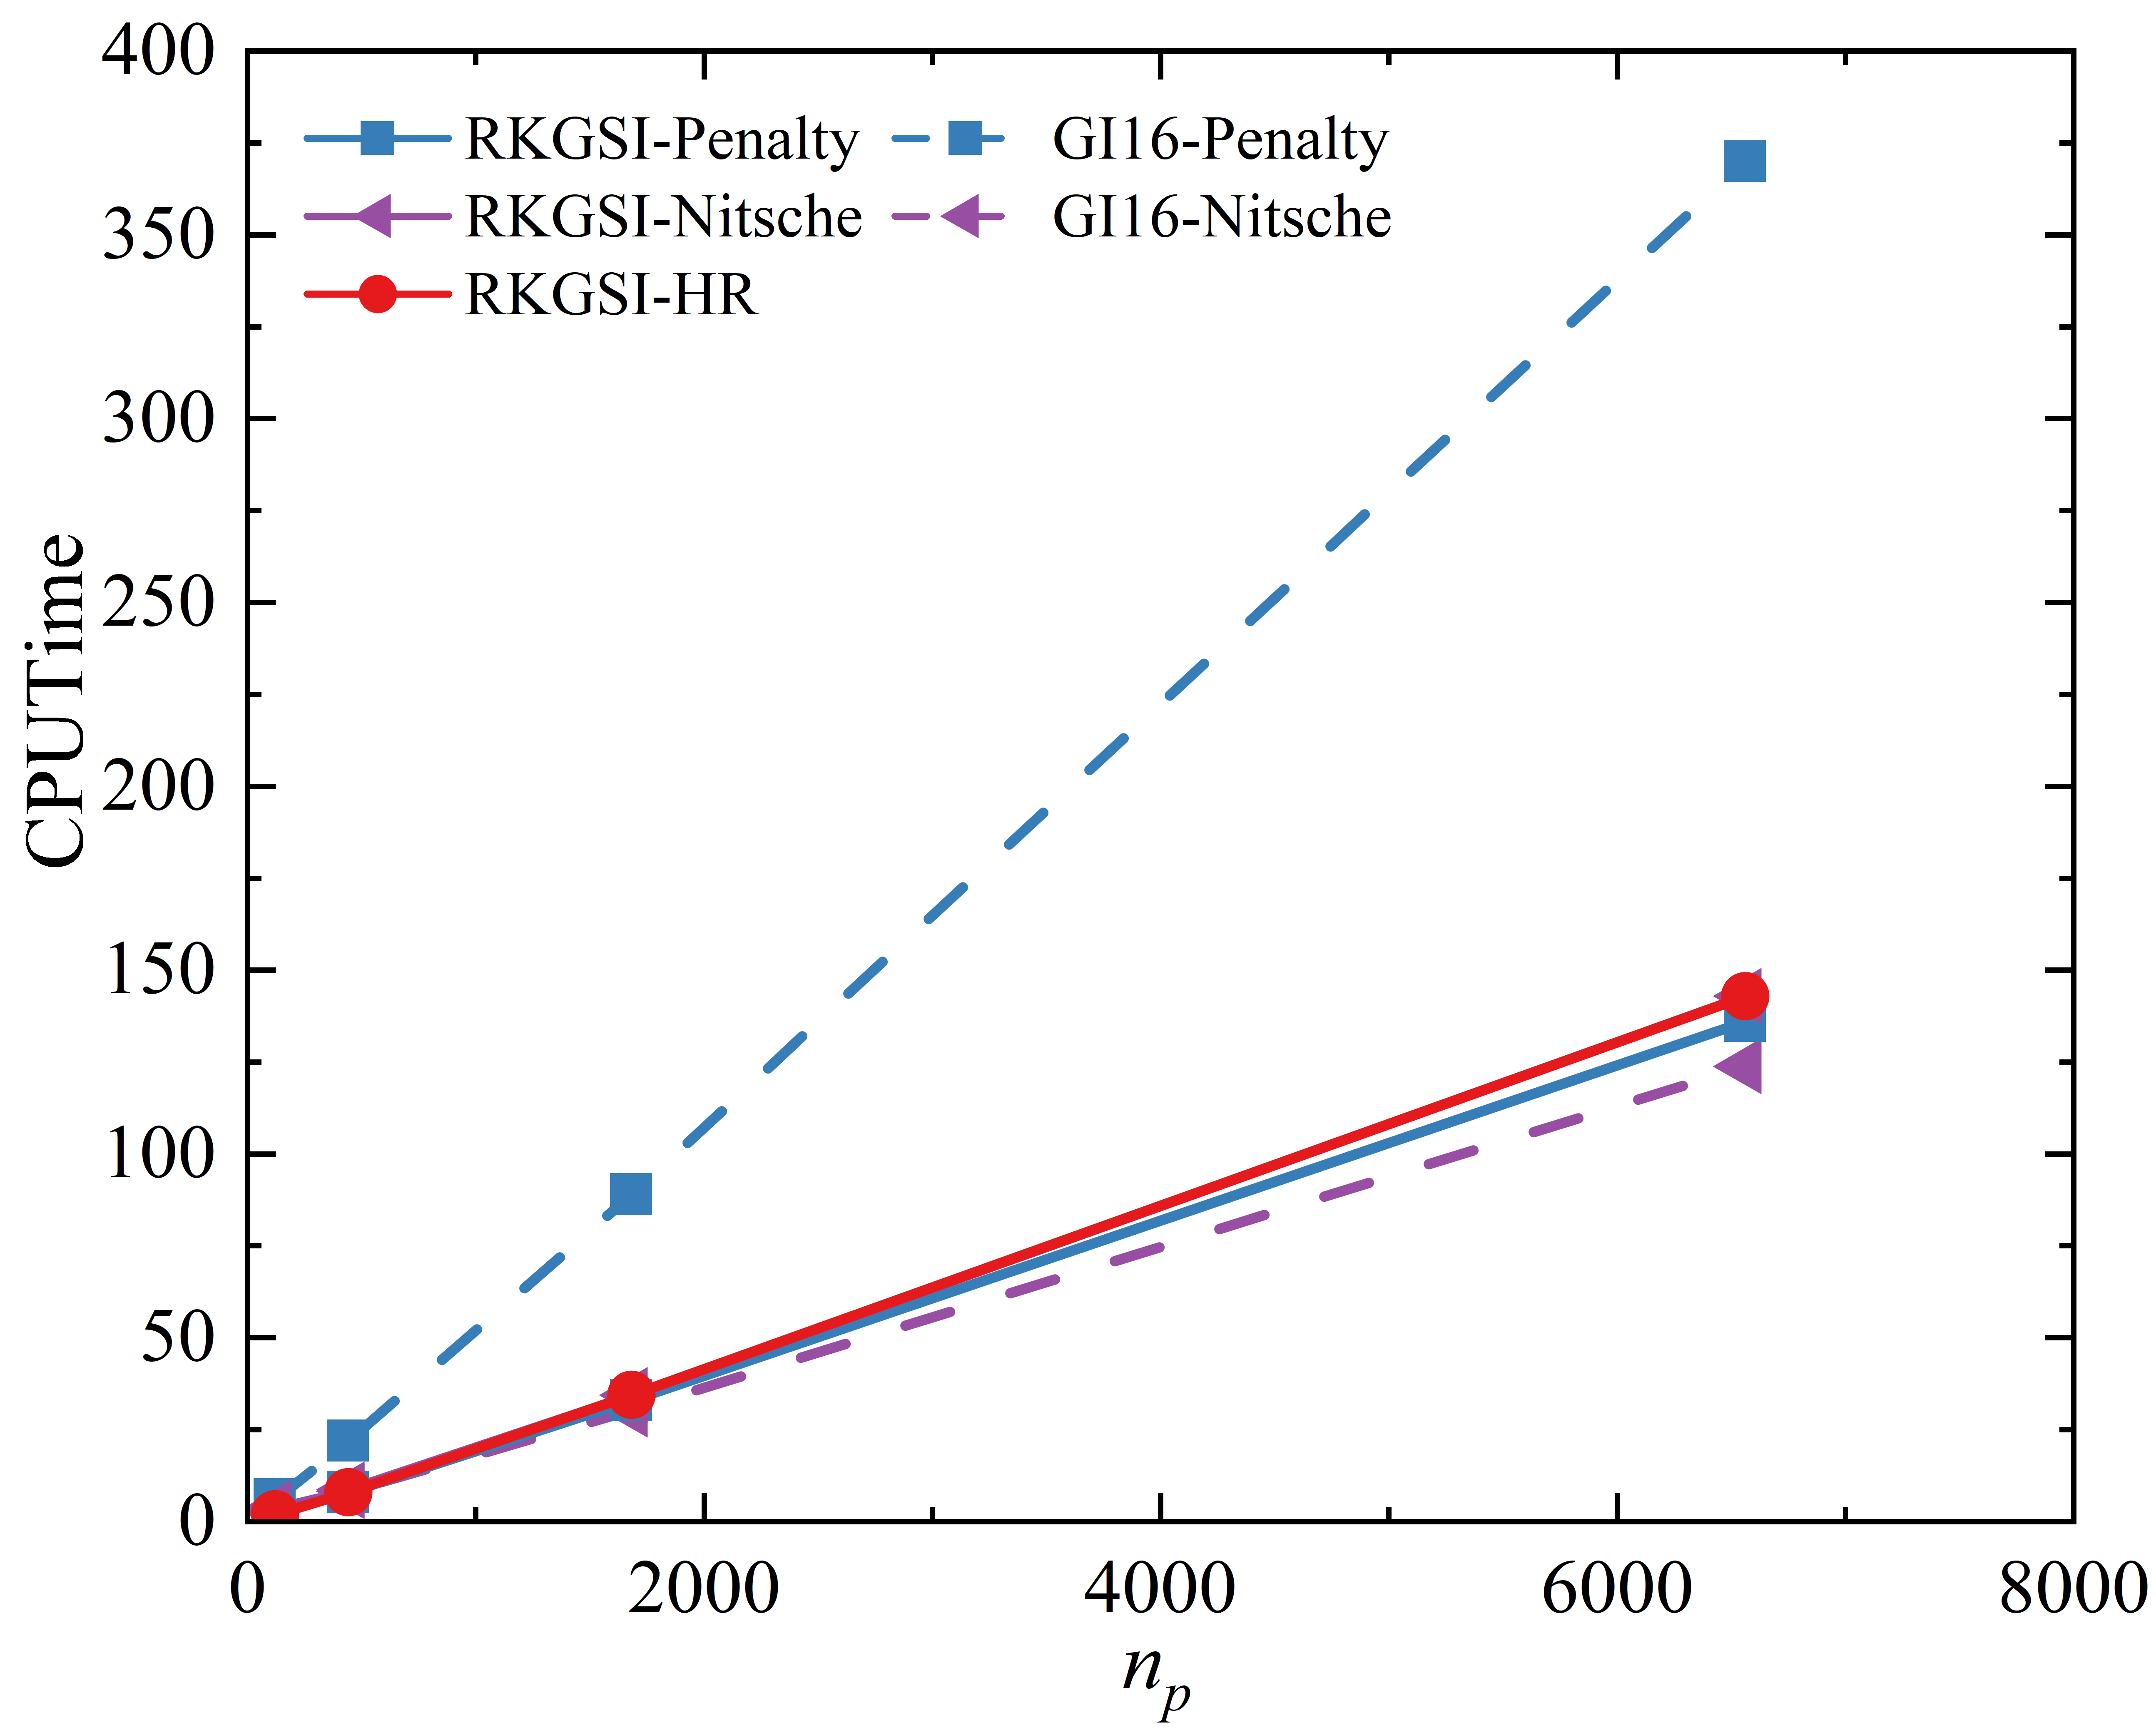
\includegraphics[width=0.49\textwidth]{figure/PHR/R/Qcputime.png}
    \phantomcaption\label{Qcputime}
    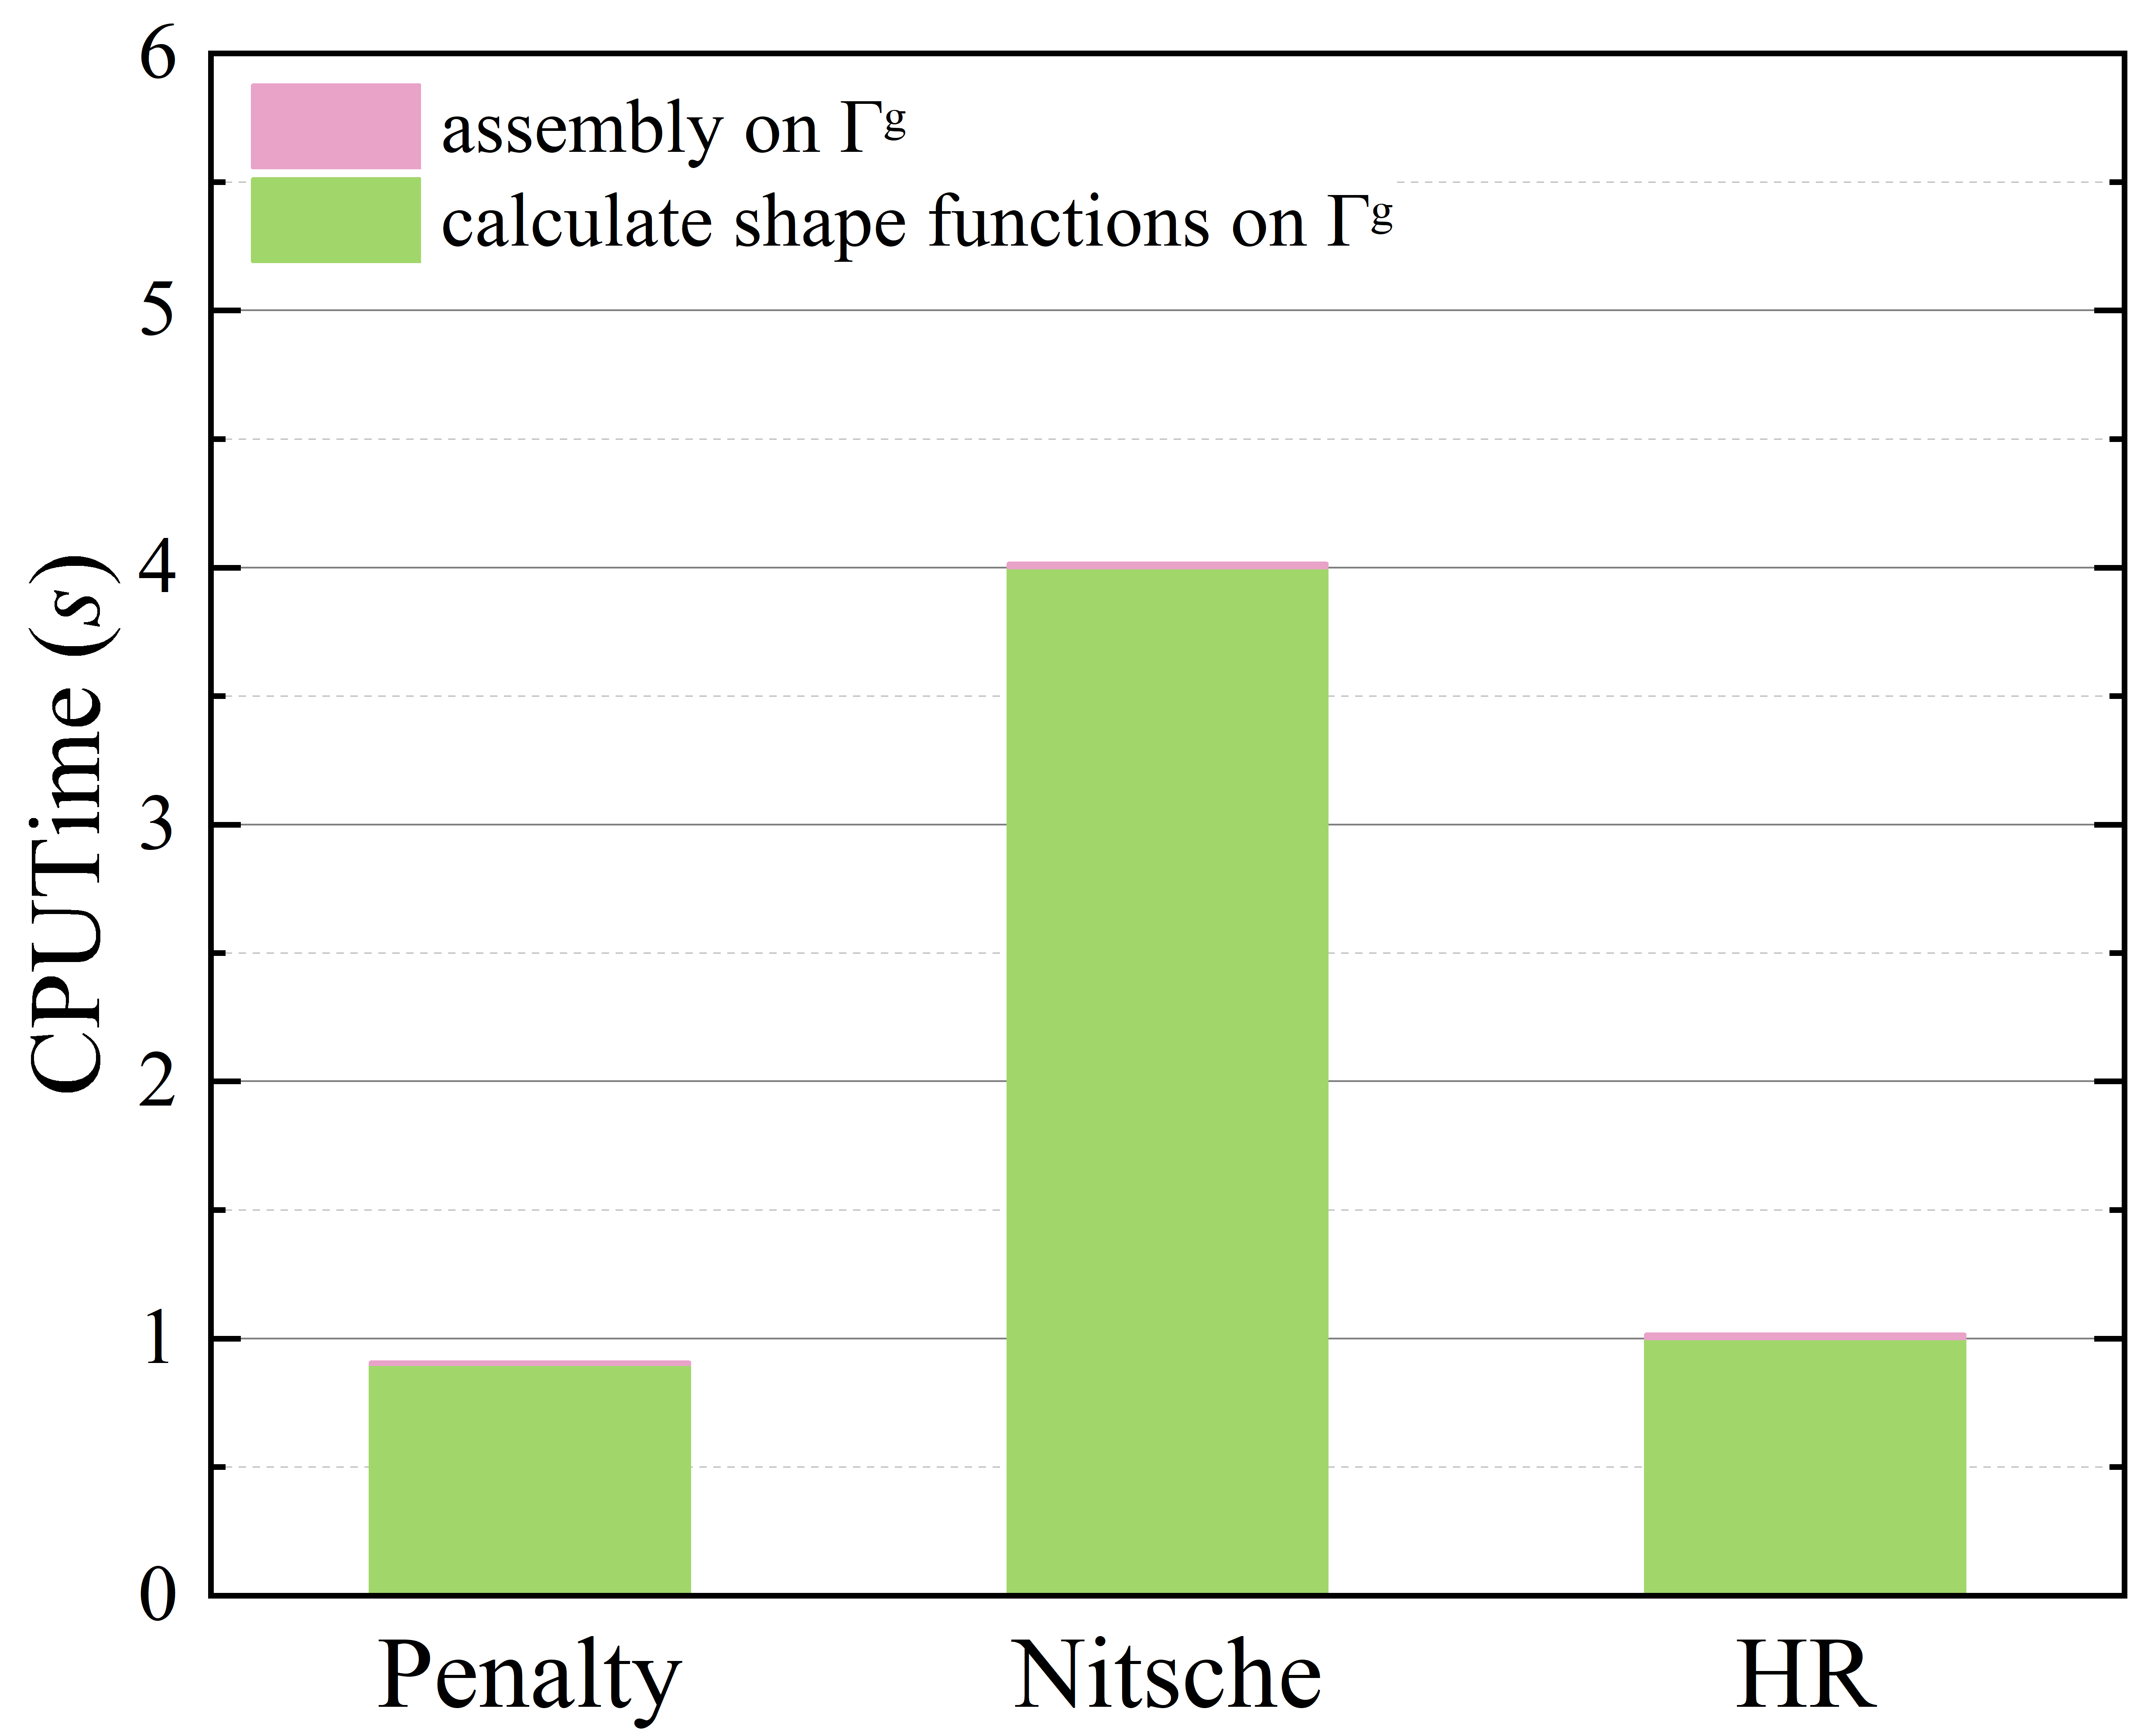
\includegraphics[width=0.49\textwidth]{figure/PHR/R/Qefficiency.png}
    \phantomcaption\label{Qefficiency}
    \end{subcaptiongroup}
\caption{简支方板问题四次基函数效率对比:\subref{Qcputime}计算时间与节点数的关系;\subref{Cefficiency}本质边界条件施加效率分析}
\label{RQcputime}
\end{figure}
图(\ref{Ralpha})是分别验证简支方板问题在三次基函数和四次基函数时带有人工经验参数的罚函数法和Nitsche法的敏感度分析。
从图中可以明显的看出,不同的经验参数对罚函数法的误差有着很大的影响,并且它的最优误差只在一小部分。
Nitsche法的最优误差的人工经验参数的范围比较大,但人工经验参数值的大小仍然会影响误差结果的变化,
并且随着网格的加密,人工经验参数的最优结果是在发生改变的。此时,提出的基于Hellinger-Reissner变分原理
中由于内嵌了本质边界条件,无需人工经验参数来满足正定性,相较于同样满足积分约束条件的“RKGSI-Nitsche”法,提出的“RKGSI-HR”法的不因人工参数值的变化影响最优误差。
\begin{figure}[H]
    \centering
    \begin{subcaptiongroup}
    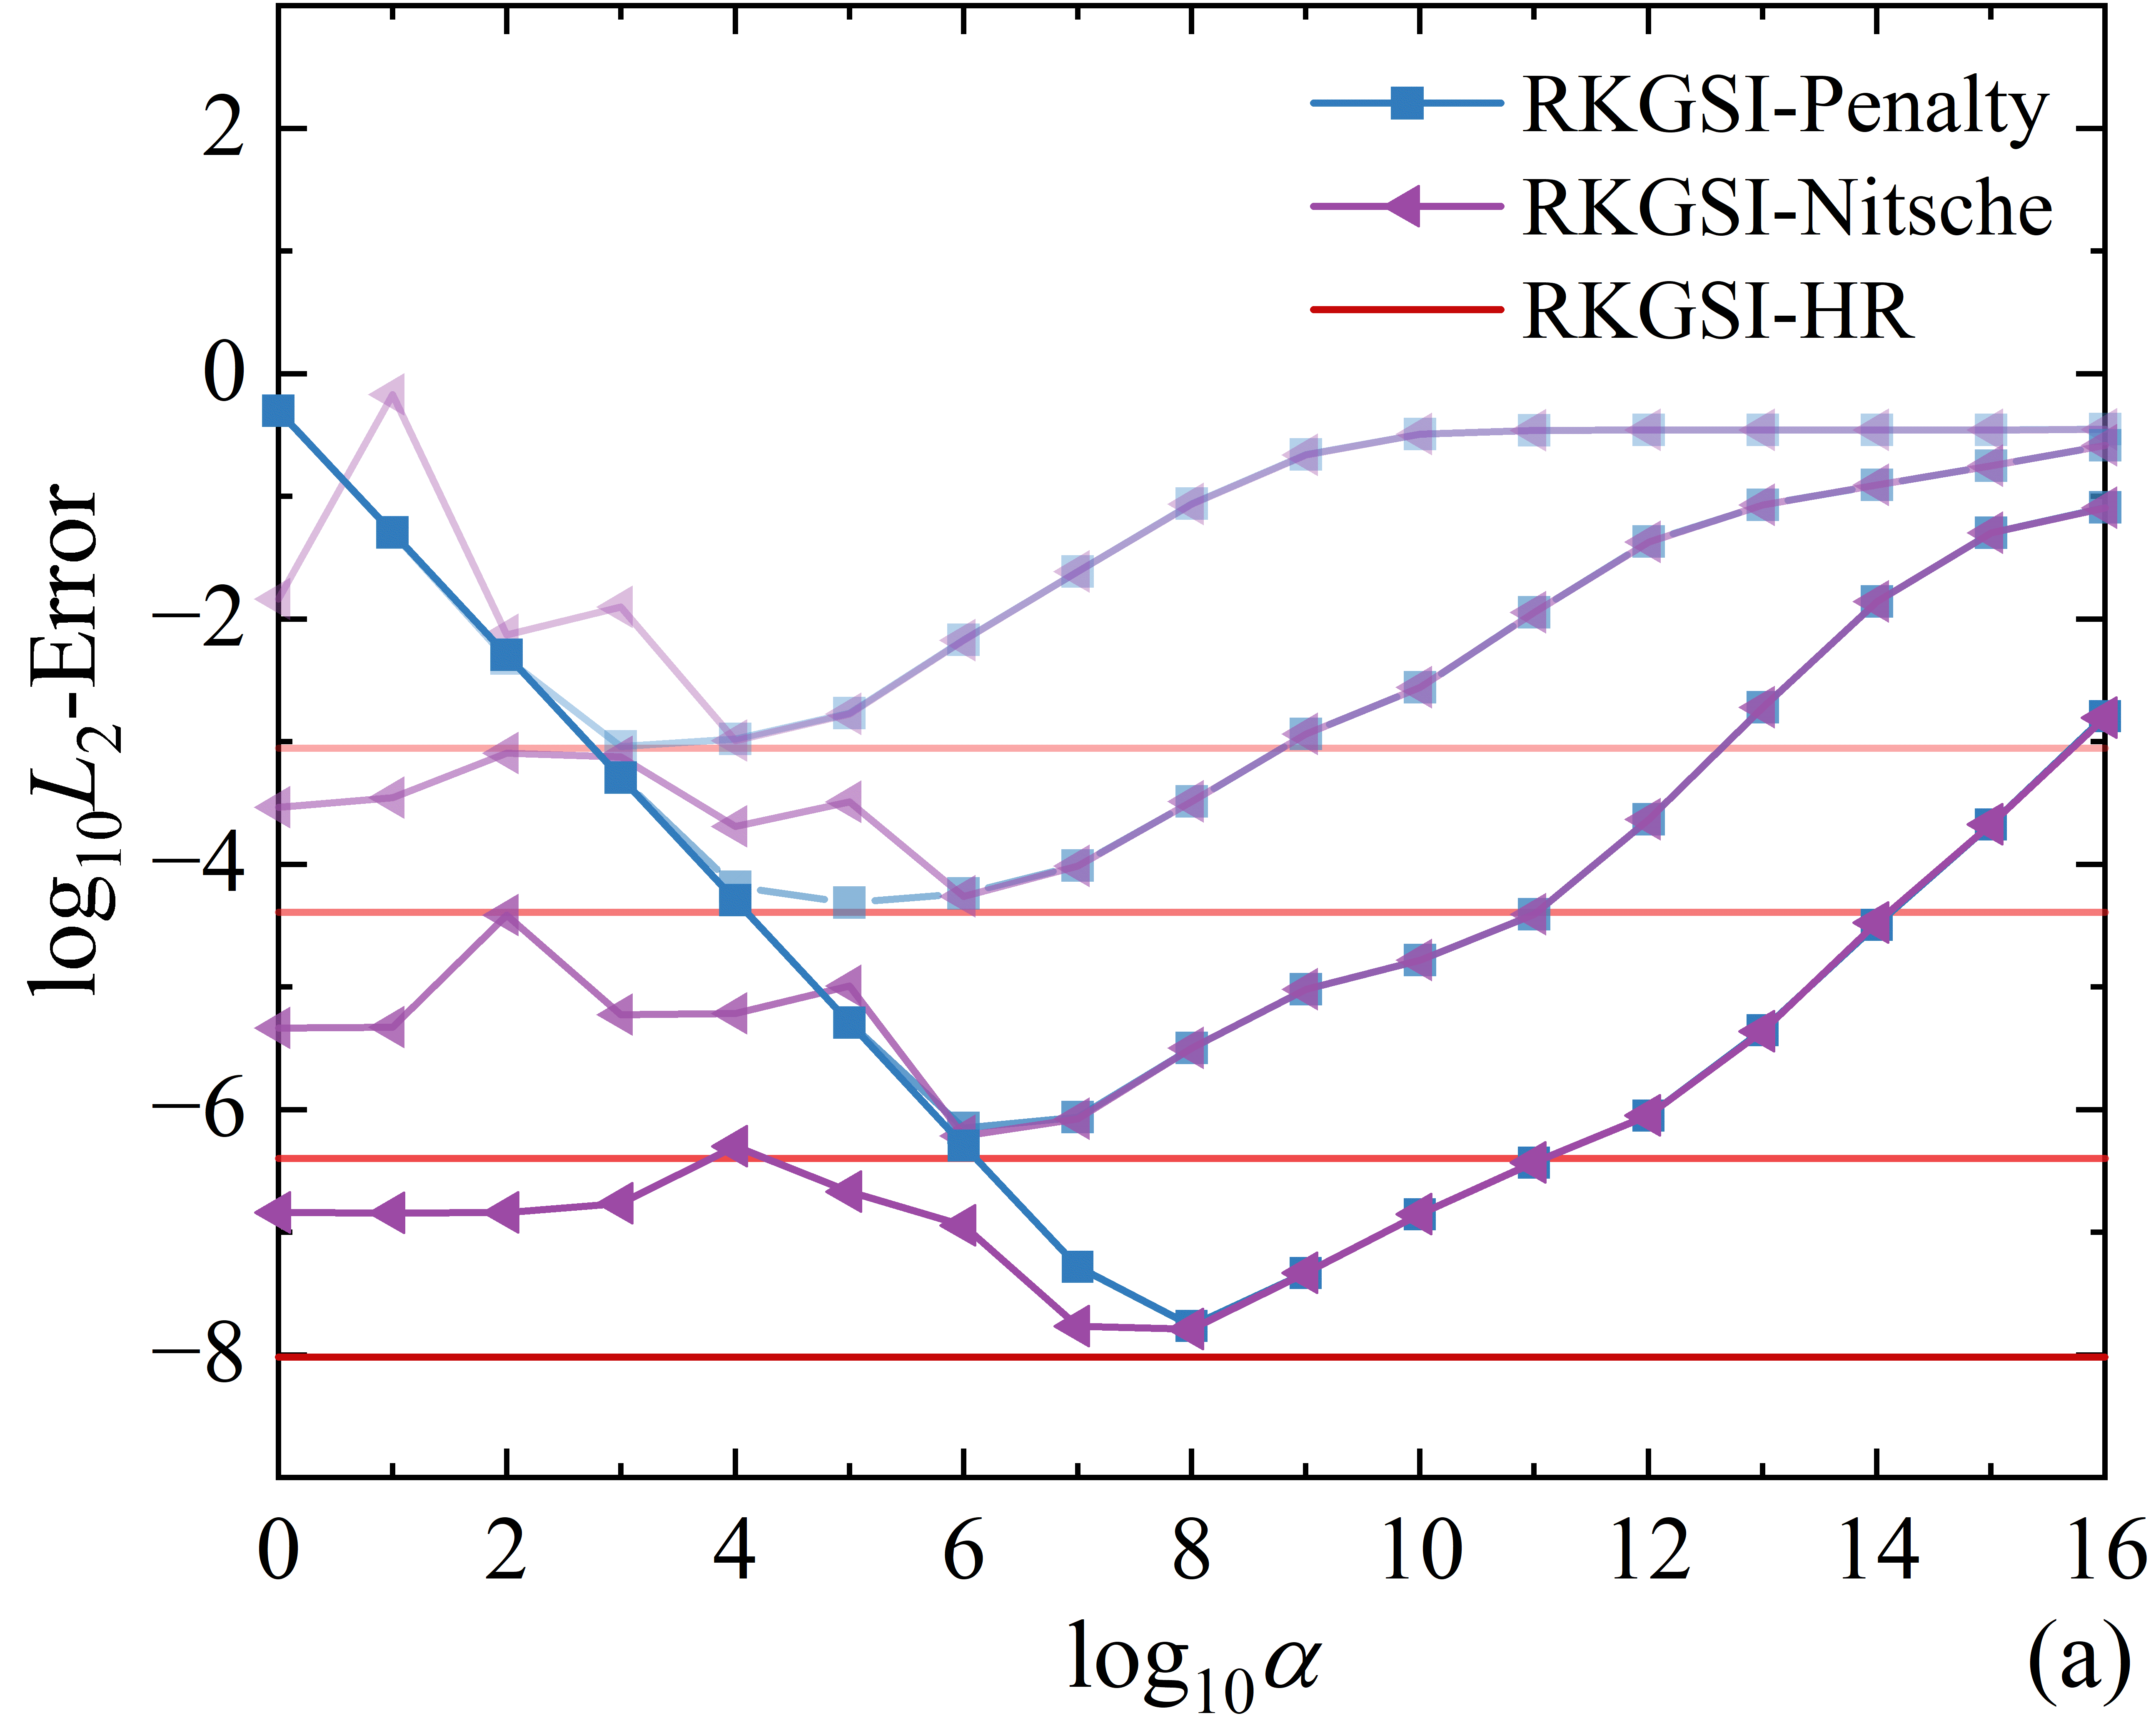
\includegraphics[width=0.49\textwidth]{figure/PHR/R/calpha.png}
    \phantomcaption\label{calpha}
    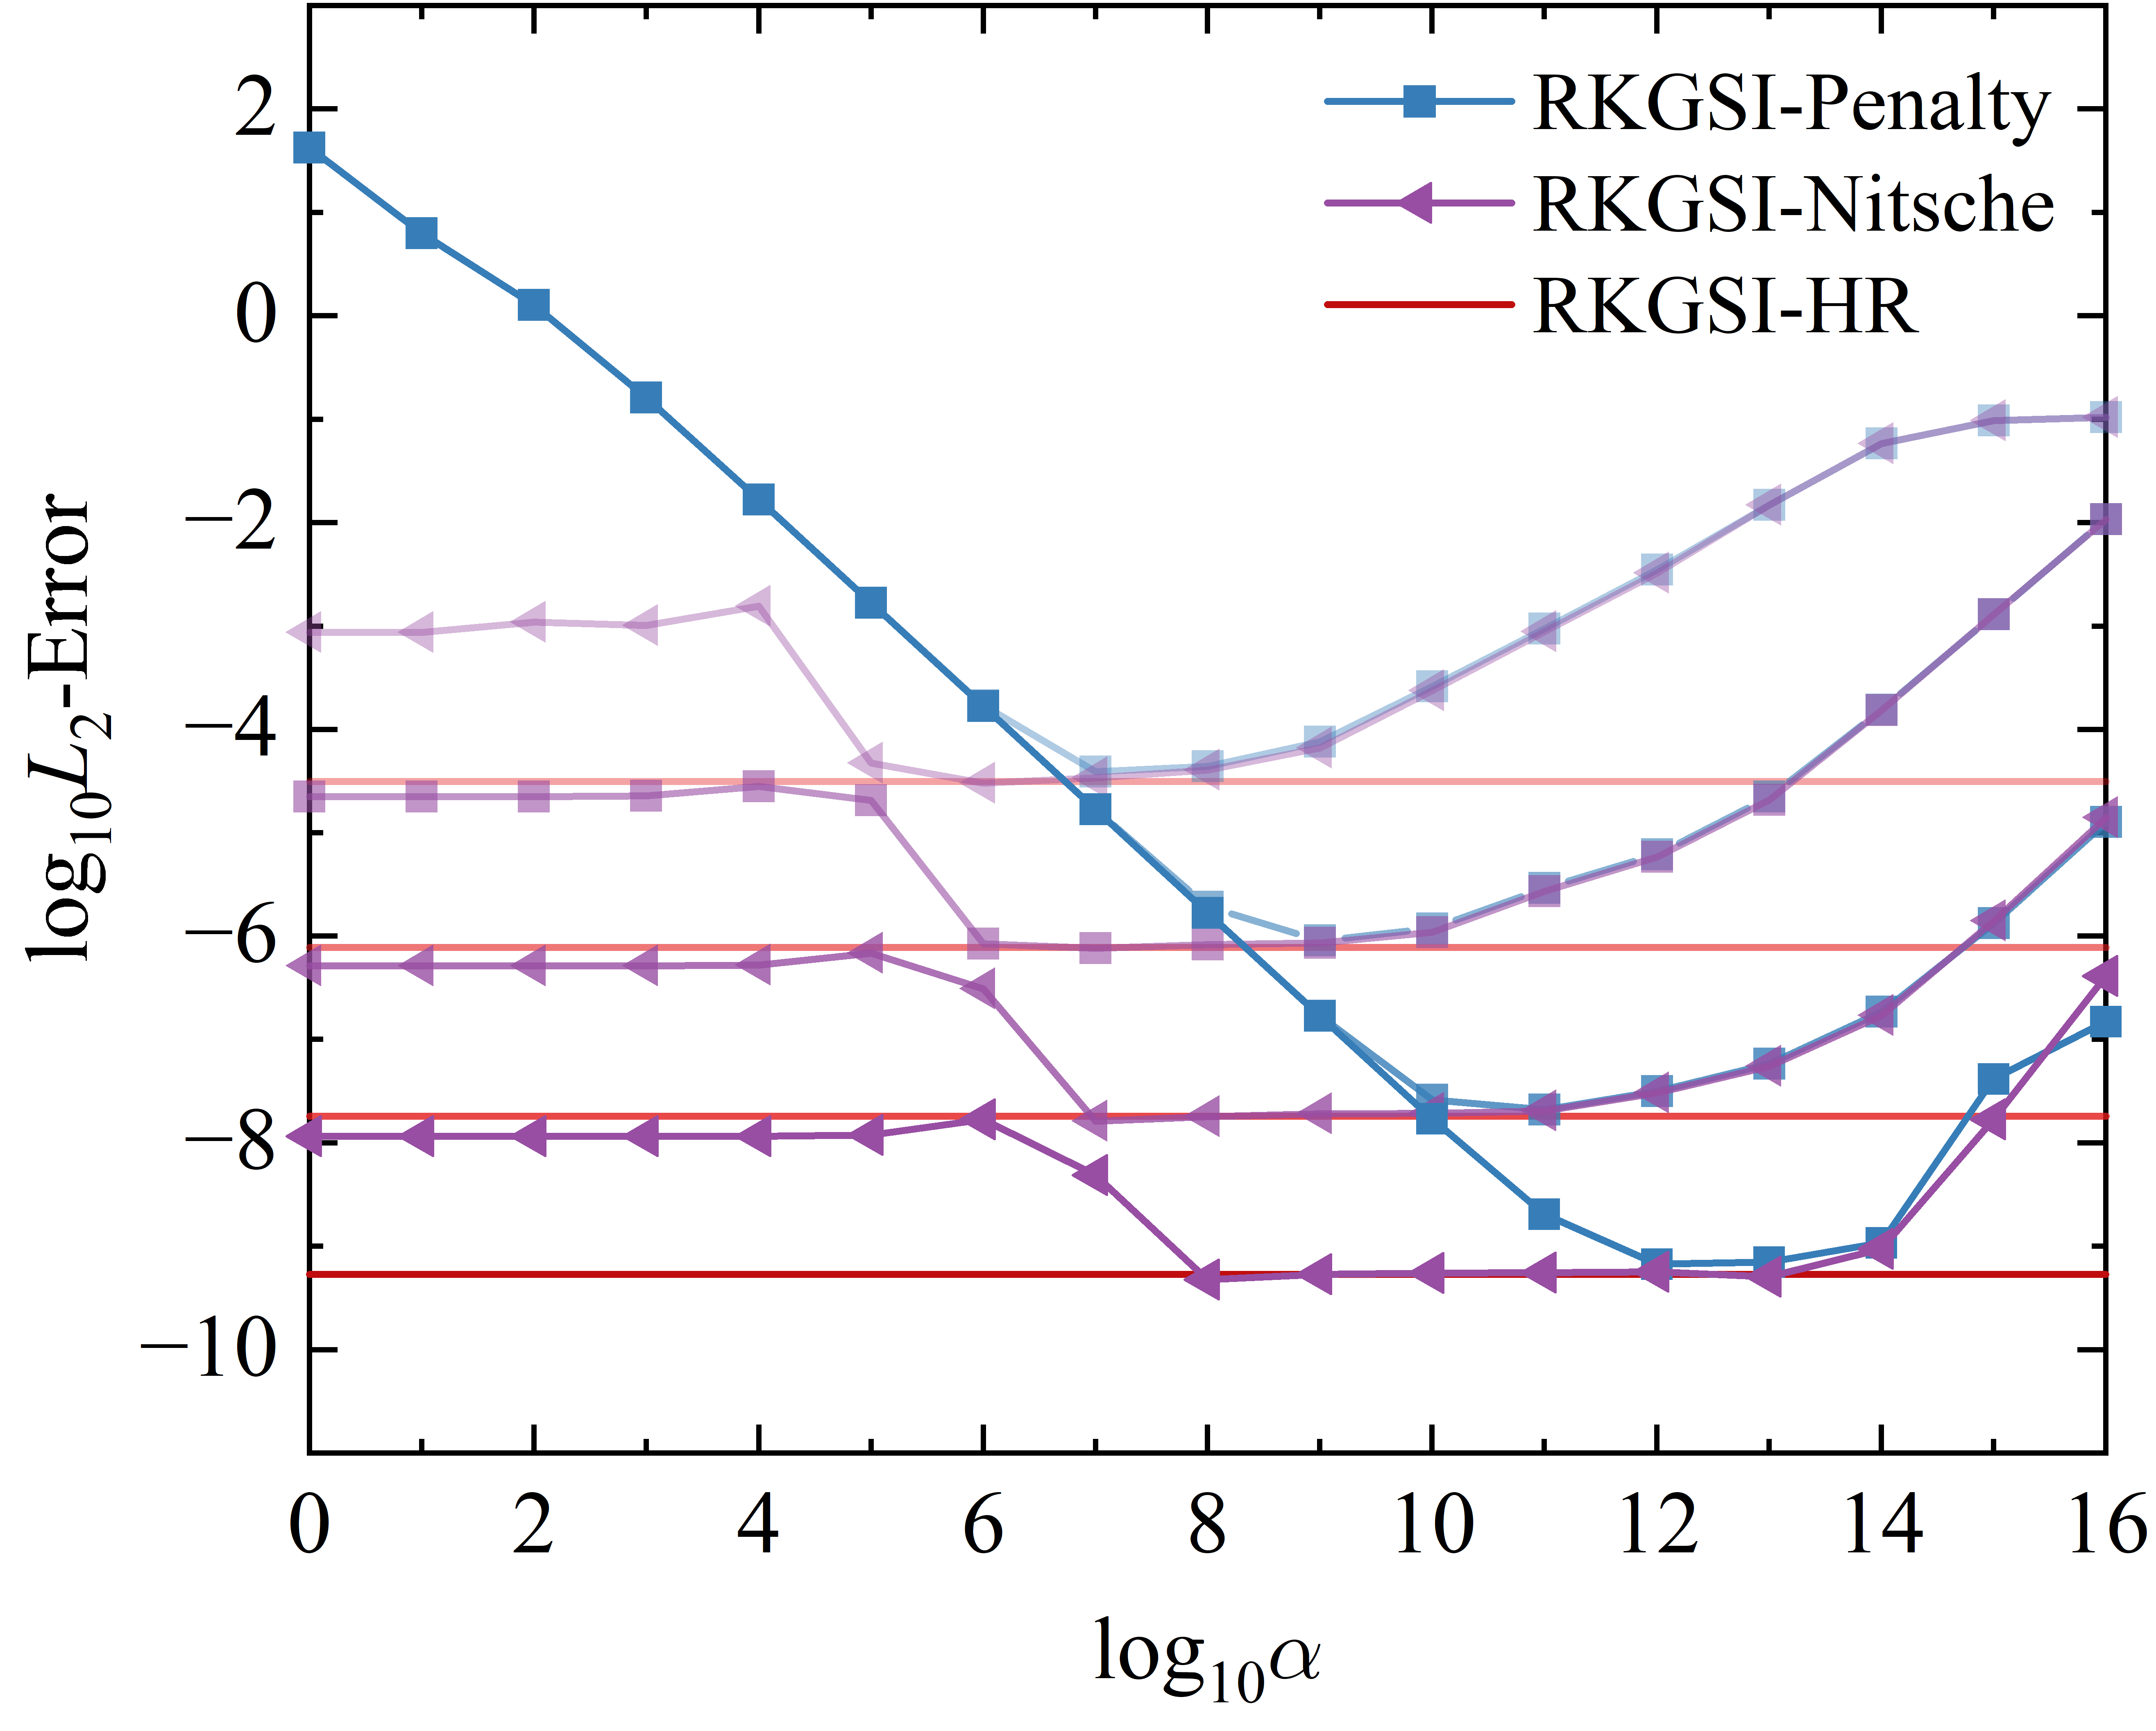
\includegraphics[width=0.49\textwidth]{figure/PHR/R/qalpha.png}
    \phantomcaption\label{qalpha}
    \end{subcaptiongroup}
\caption{人工参数$\alpha$敏感度分析:\subref{calpha}三次基函数;\subref{qalpha}四次基函数}
\label{Ralpha}
\end{figure}
\newpage
\subsection{简支等边三角形板问题}
考虑如图(\ref{triangular})所示简支等边三角形板,其中三角形板的高为$a=10$,均布荷载作用在板面内为$\bar{q}=1$,材料系数分别为弯曲刚度$\bar{D}=1$、泊松比$\nu=0.3$。该简支三角形板的精确解为:
\begin{equation}
\begin{split}
    w=\frac{\bar q}{64a\bar D}[x^3-3y^3x-a(x^2+y^2)+\frac{4}{27}a^3](\frac{4}{9}a^2-x^2-y^2)
\end{split}
\end{equation}\par
如图(\ref{triangularmsh})所示,简支等边三角形板求解域分布采用均布离散的66、231、861和3321的四个疏密不同的节点进行离散。同样采用三次基函数时,简支等边三角形板问题的相对影响域取为3.5,四次基函数时其相对应影响域取为4.5进行数值分析。\par
\begin{figure}[H]
    \centering
    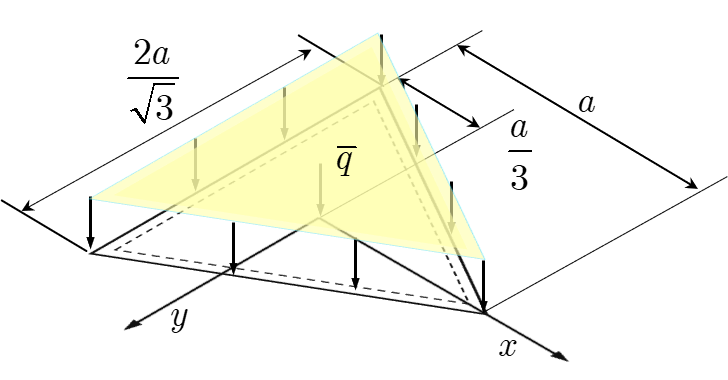
\includegraphics[scale=0.7]{figure/PHR/T/triangular.png}
    \caption{简支等边三角形板问题模型}\label{triangular}
\end{figure}
\begin{figure}[H]
    \centering
    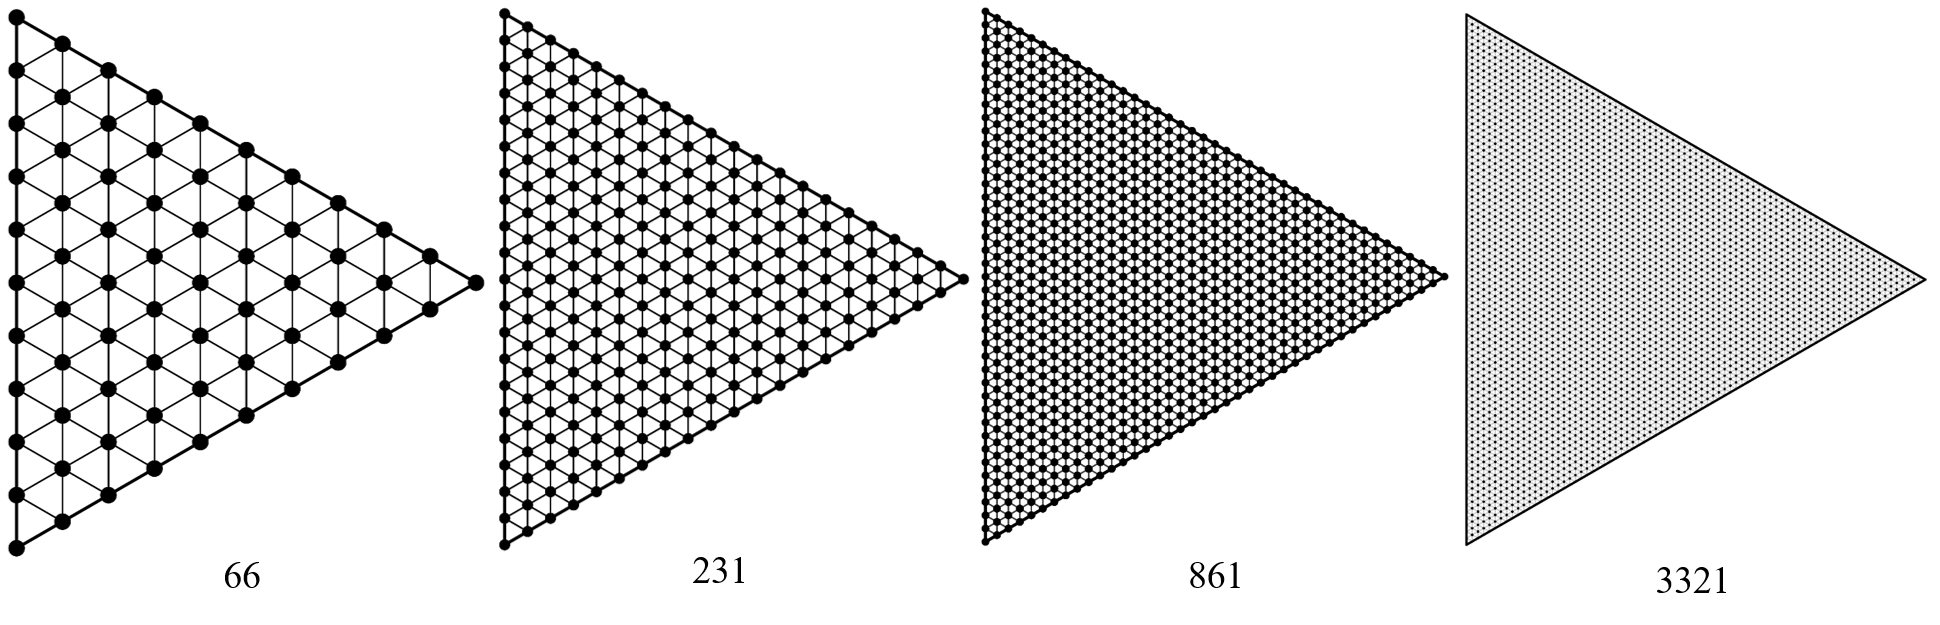
\includegraphics[scale=0.4]{figure/PHR/T/triangularmsh.png}
    \caption{简支等边三角形问题节点离散}\label{triangularmsh}
\end{figure}
图(\ref{TCLH})、图(\ref{TQLH})为简支等边三角形板问题分别在三次基函数和四次基函数的位移误差和能量误差对比图。
从图中可以明显看出采用“RKGSI”得出的计算精度优于“GI”法,
并且“RKGSI-HR”法都能够达到理论误差收敛率,满足积分约束条件。
图(\ref{Tefficiency})是简支等边三角形板的薄板中面和本质边界条件施加效率分析图,从图中可以看出在薄板中面施加过程中,“RKGSI”所用的时间都明显少于“GI”;
而针对“RKGSI”在施加本质边界过程中计算形函数及梯度和组装相对应的刚度矩阵和力向量中可以明显看出“RKGSI-Nistche”法所用的时间明显多于“RKGSI-HR”法,
% 虽然“RKGSI-HR”和“RKGSI-Penalty”的计算效率相差不大,但“RKGSI-Penalty”由于不具有变分一致性无法达到理论误差收敛率。
% 因此相较于传统的本质边界条件施加方法,“RKGSI-HR”不仅满足积分约束条件能够达到理论误差收敛率,提高计算精度,在计算时间上也用时较短,有效提高计算效率。
图(\ref{TMxy})为简支等边三角形板问题的弯矩云图。从图中可以看出“RKGSI-HR”、“RKGSI-Nitsche”和“RKGSI-Penalty”和精确解之间非常一致,进一步验证了所提方法能够有效提高计算精度。
\begin{figure}[H]
    \centering
    \begin{subcaptiongroup}
    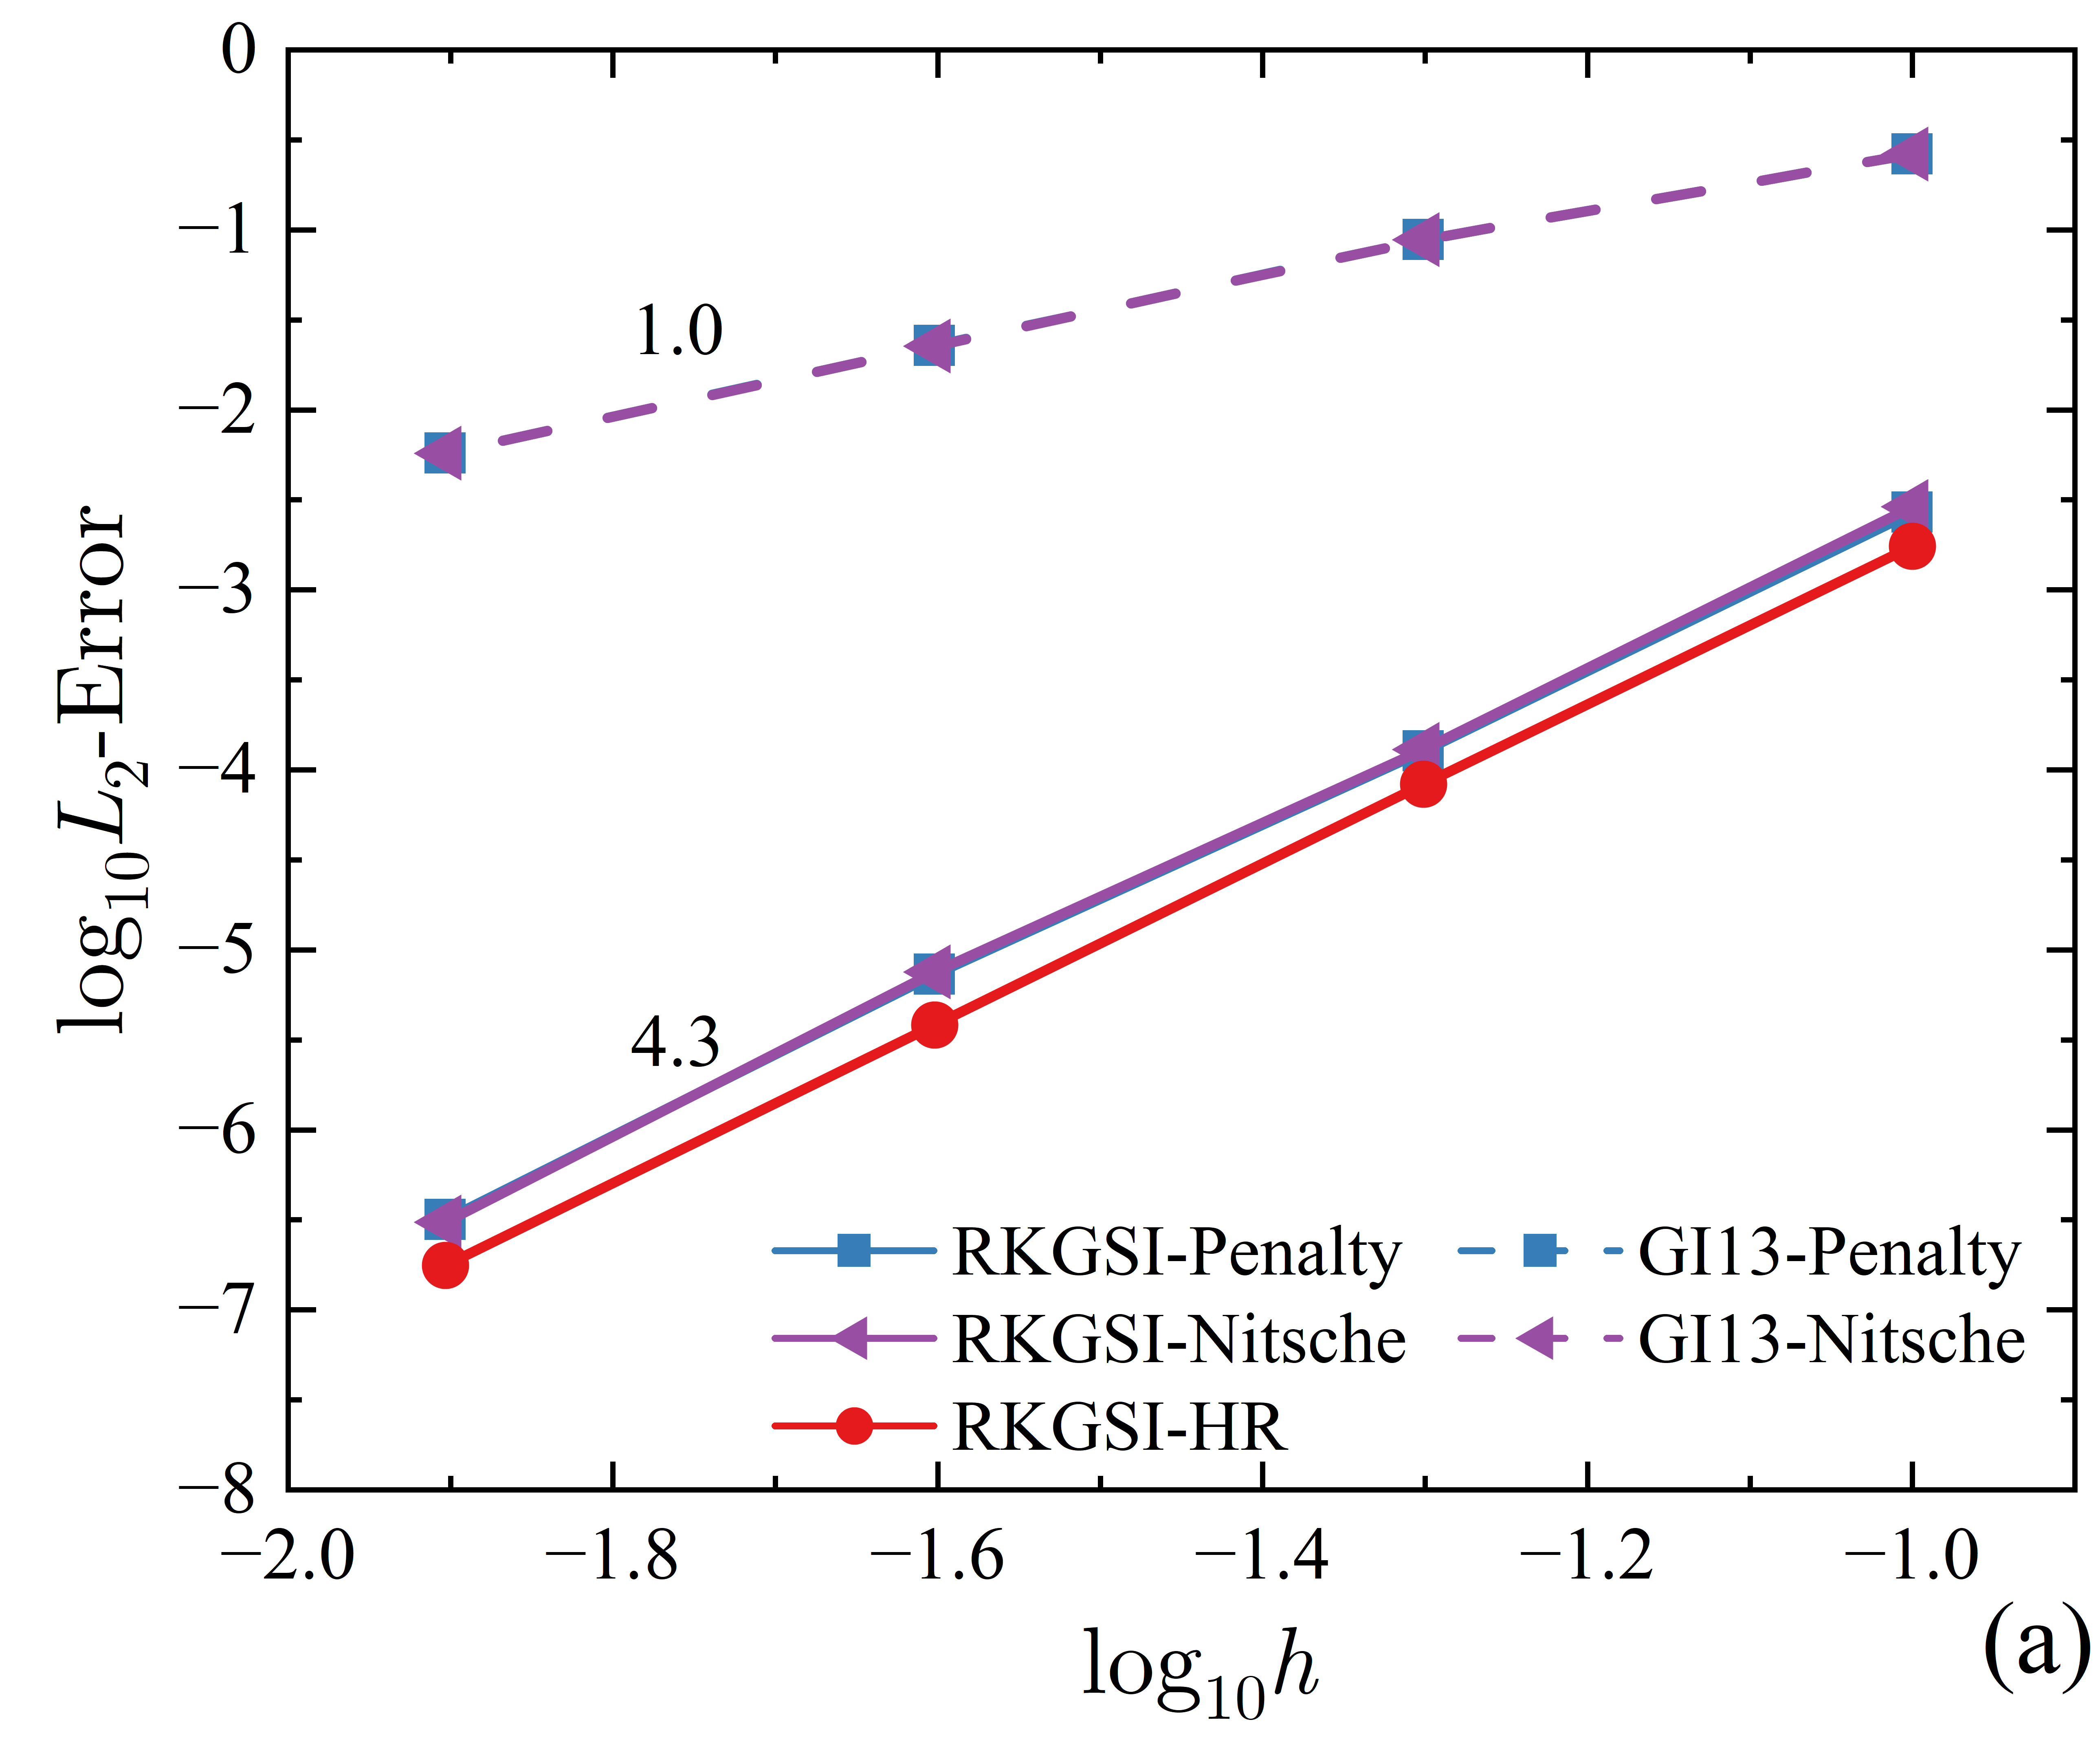
\includegraphics[width=0.49\textwidth]{figure/PHR/T/CL2.png}
    \phantomcaption\label{CL2}
    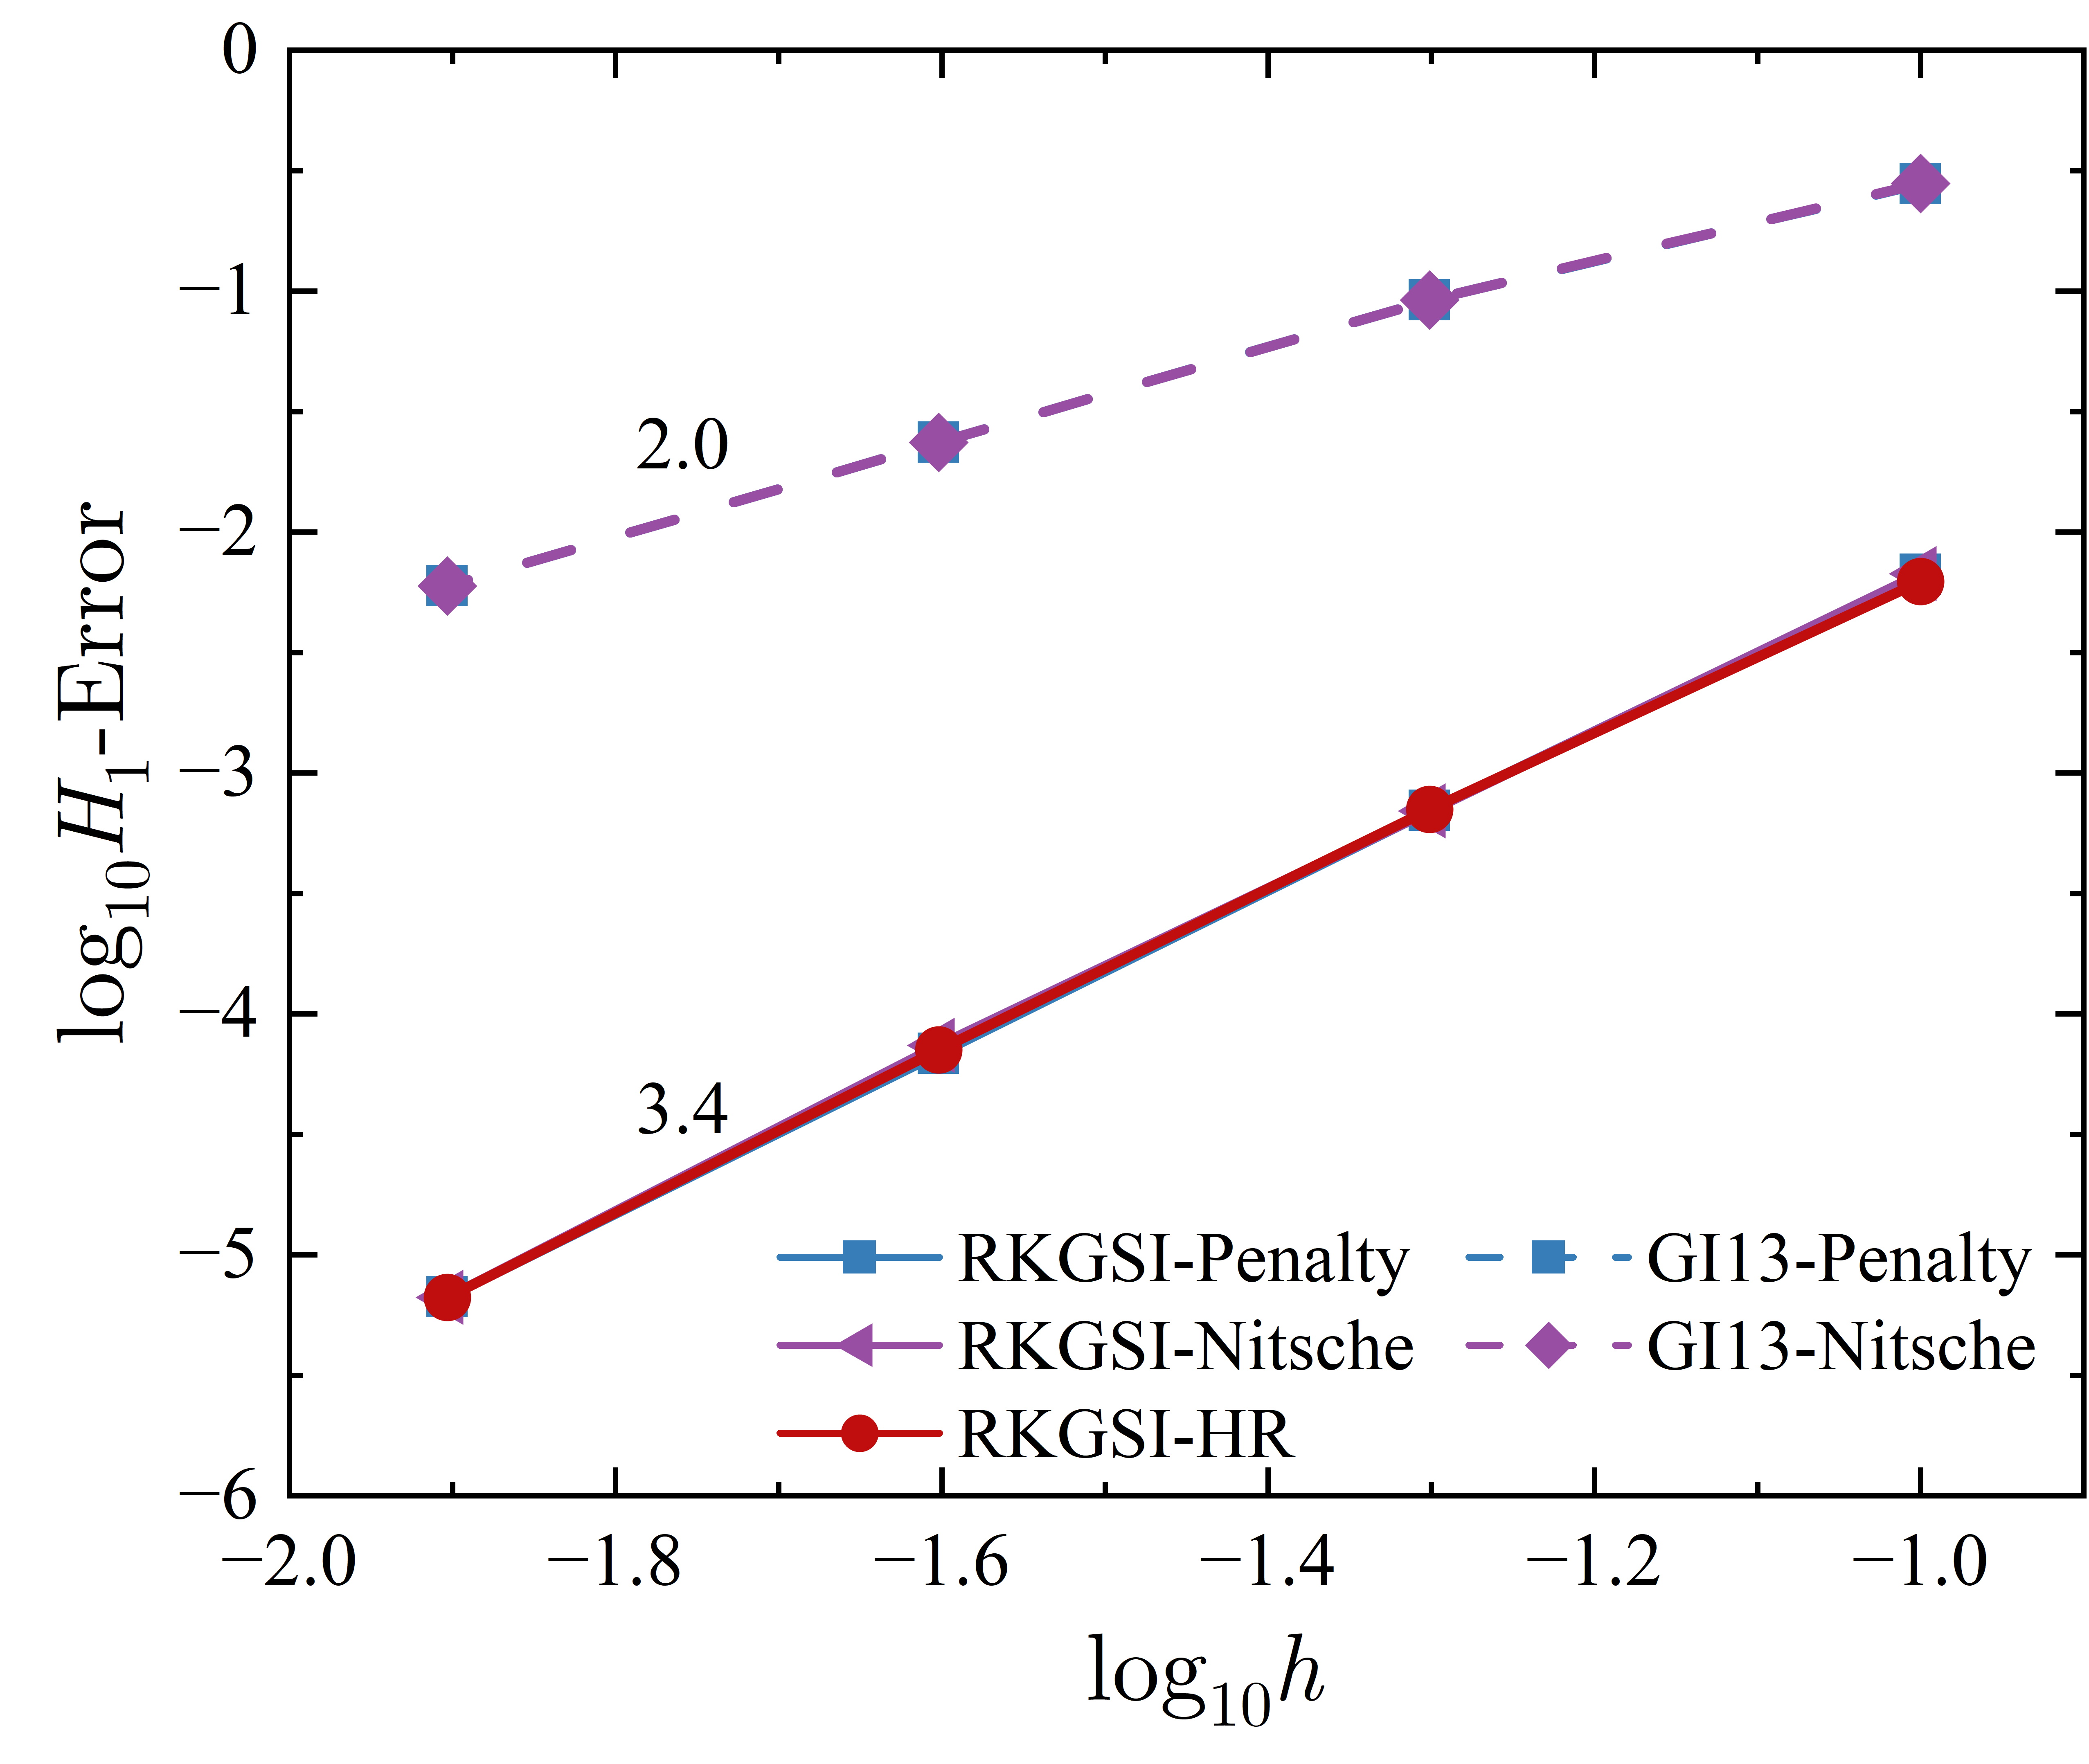
\includegraphics[width=0.49\textwidth]{figure/PHR/T/CH1.png}
    \phantomcaption\label{CH1}
    \end{subcaptiongroup}
    \begin{subcaptiongroup}
    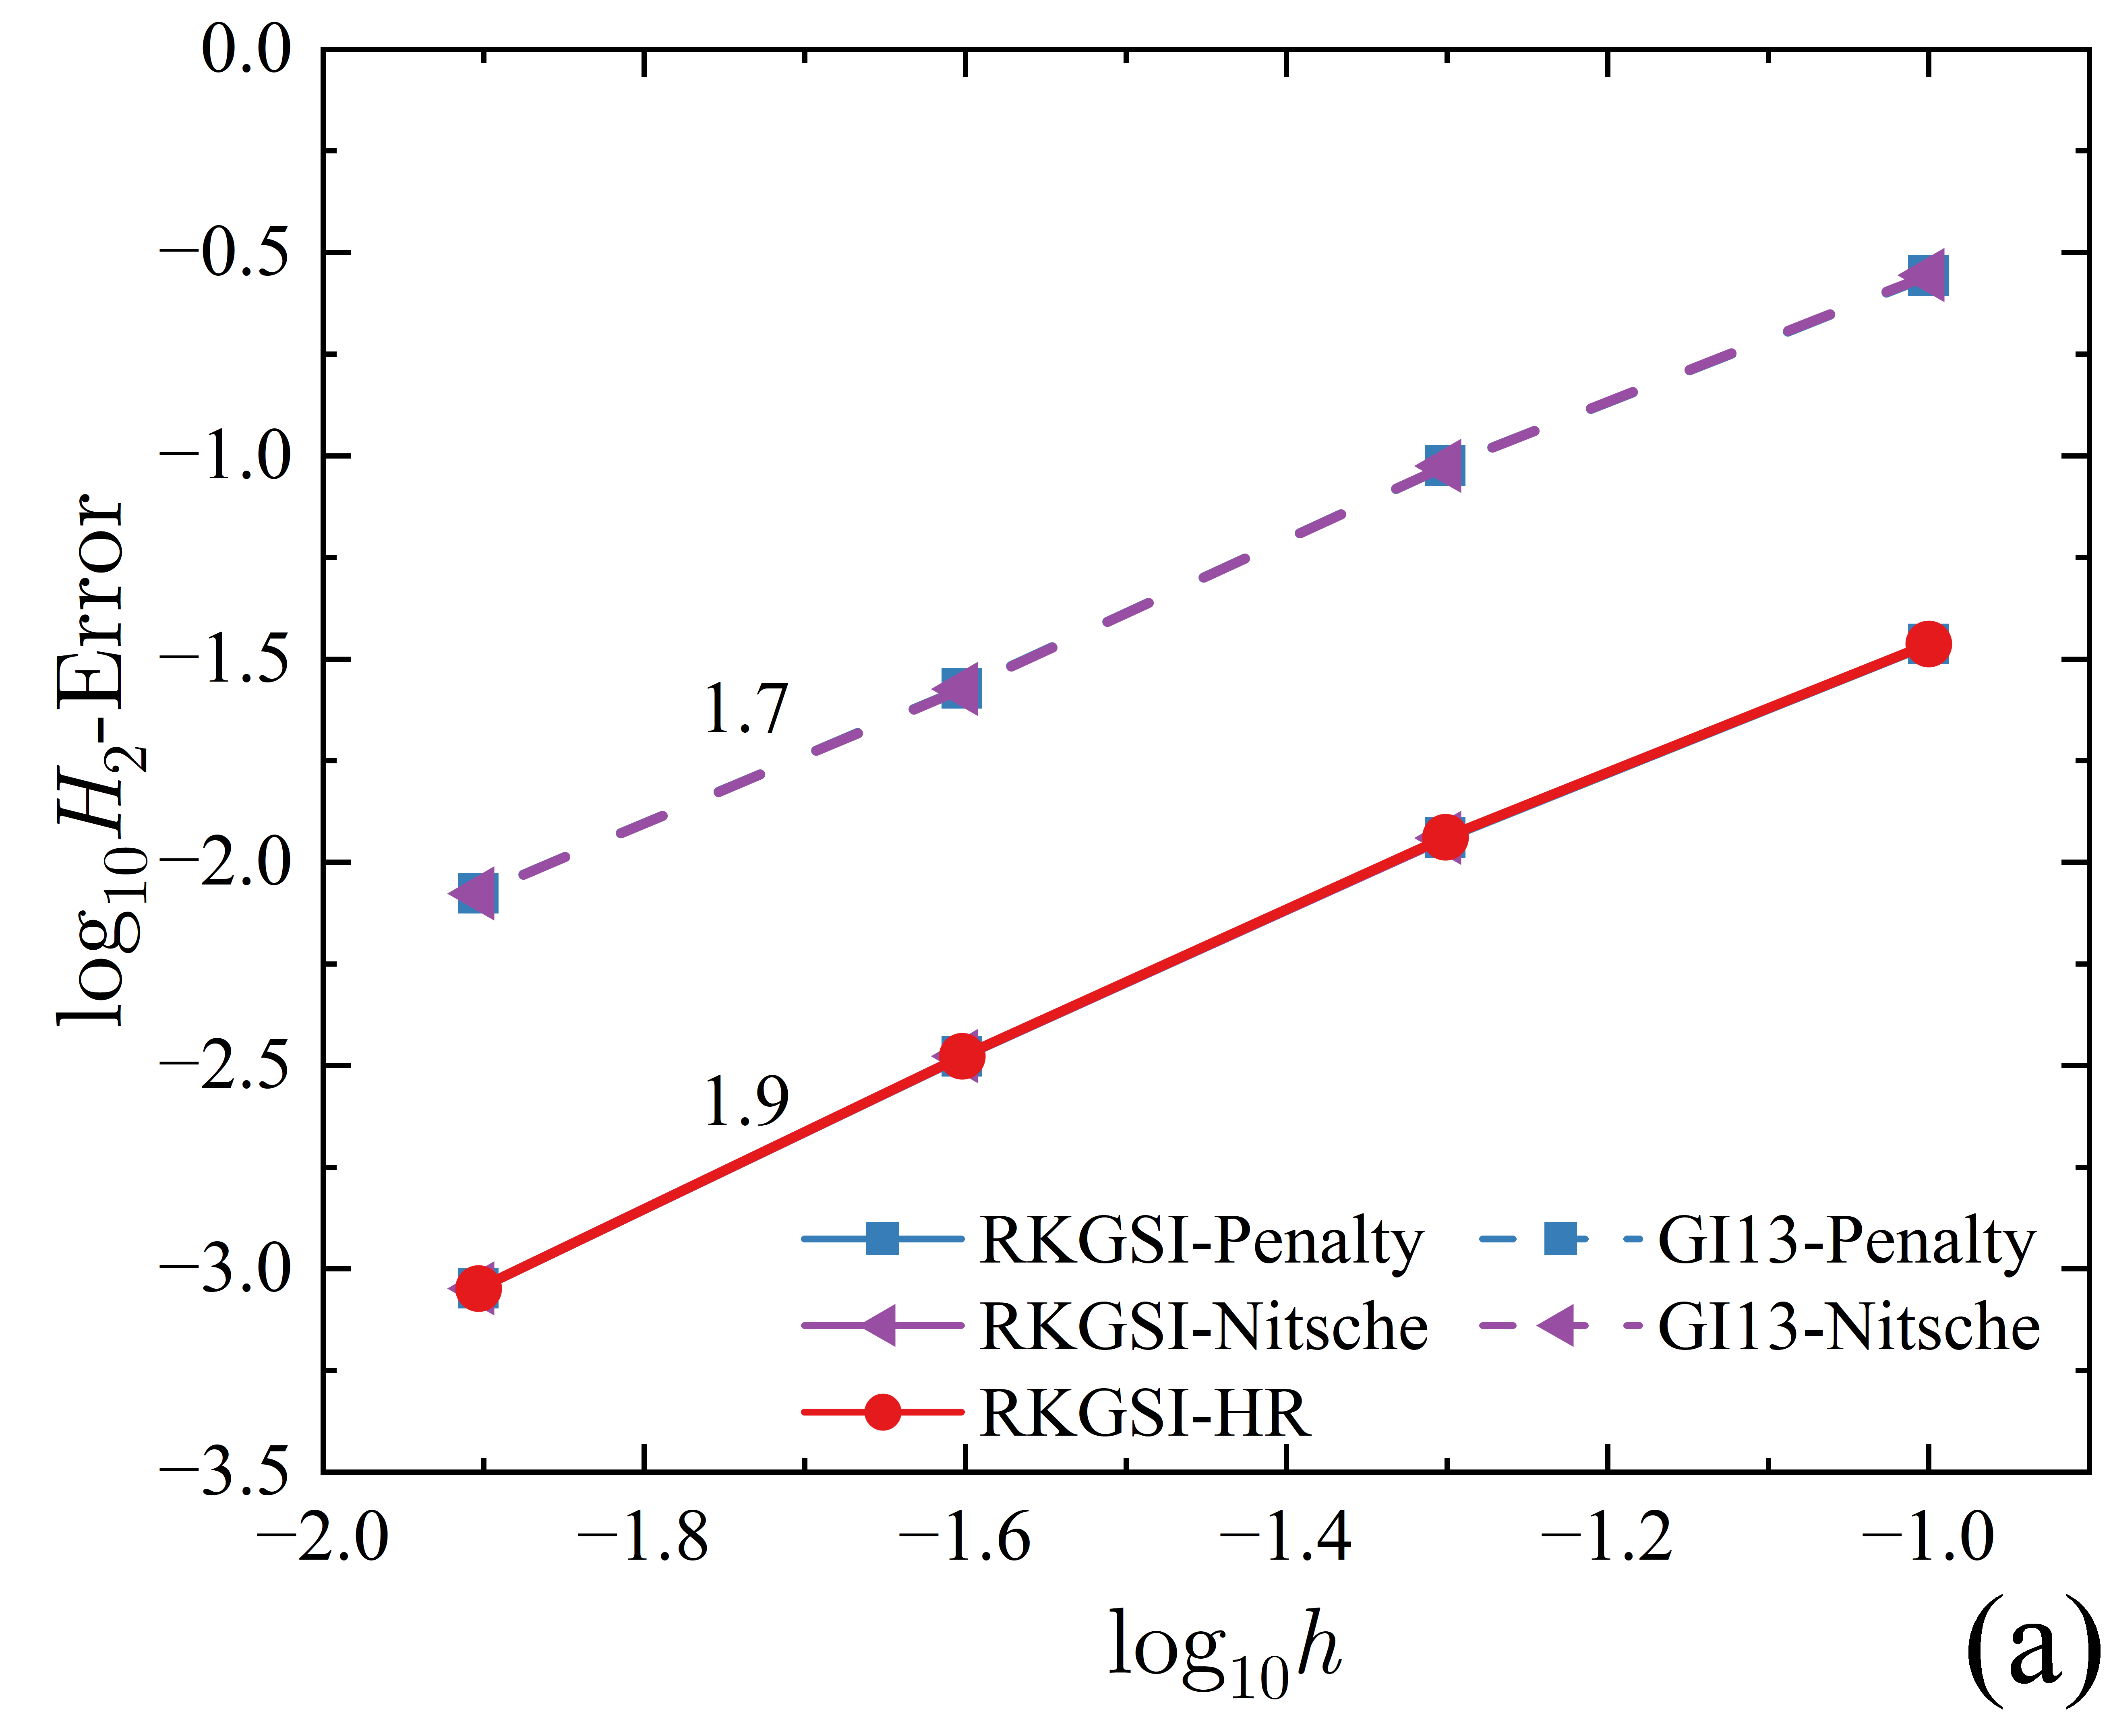
\includegraphics[width=0.49\textwidth]{figure/PHR/T/CH2.png}
    \phantomcaption\label{CH2}
    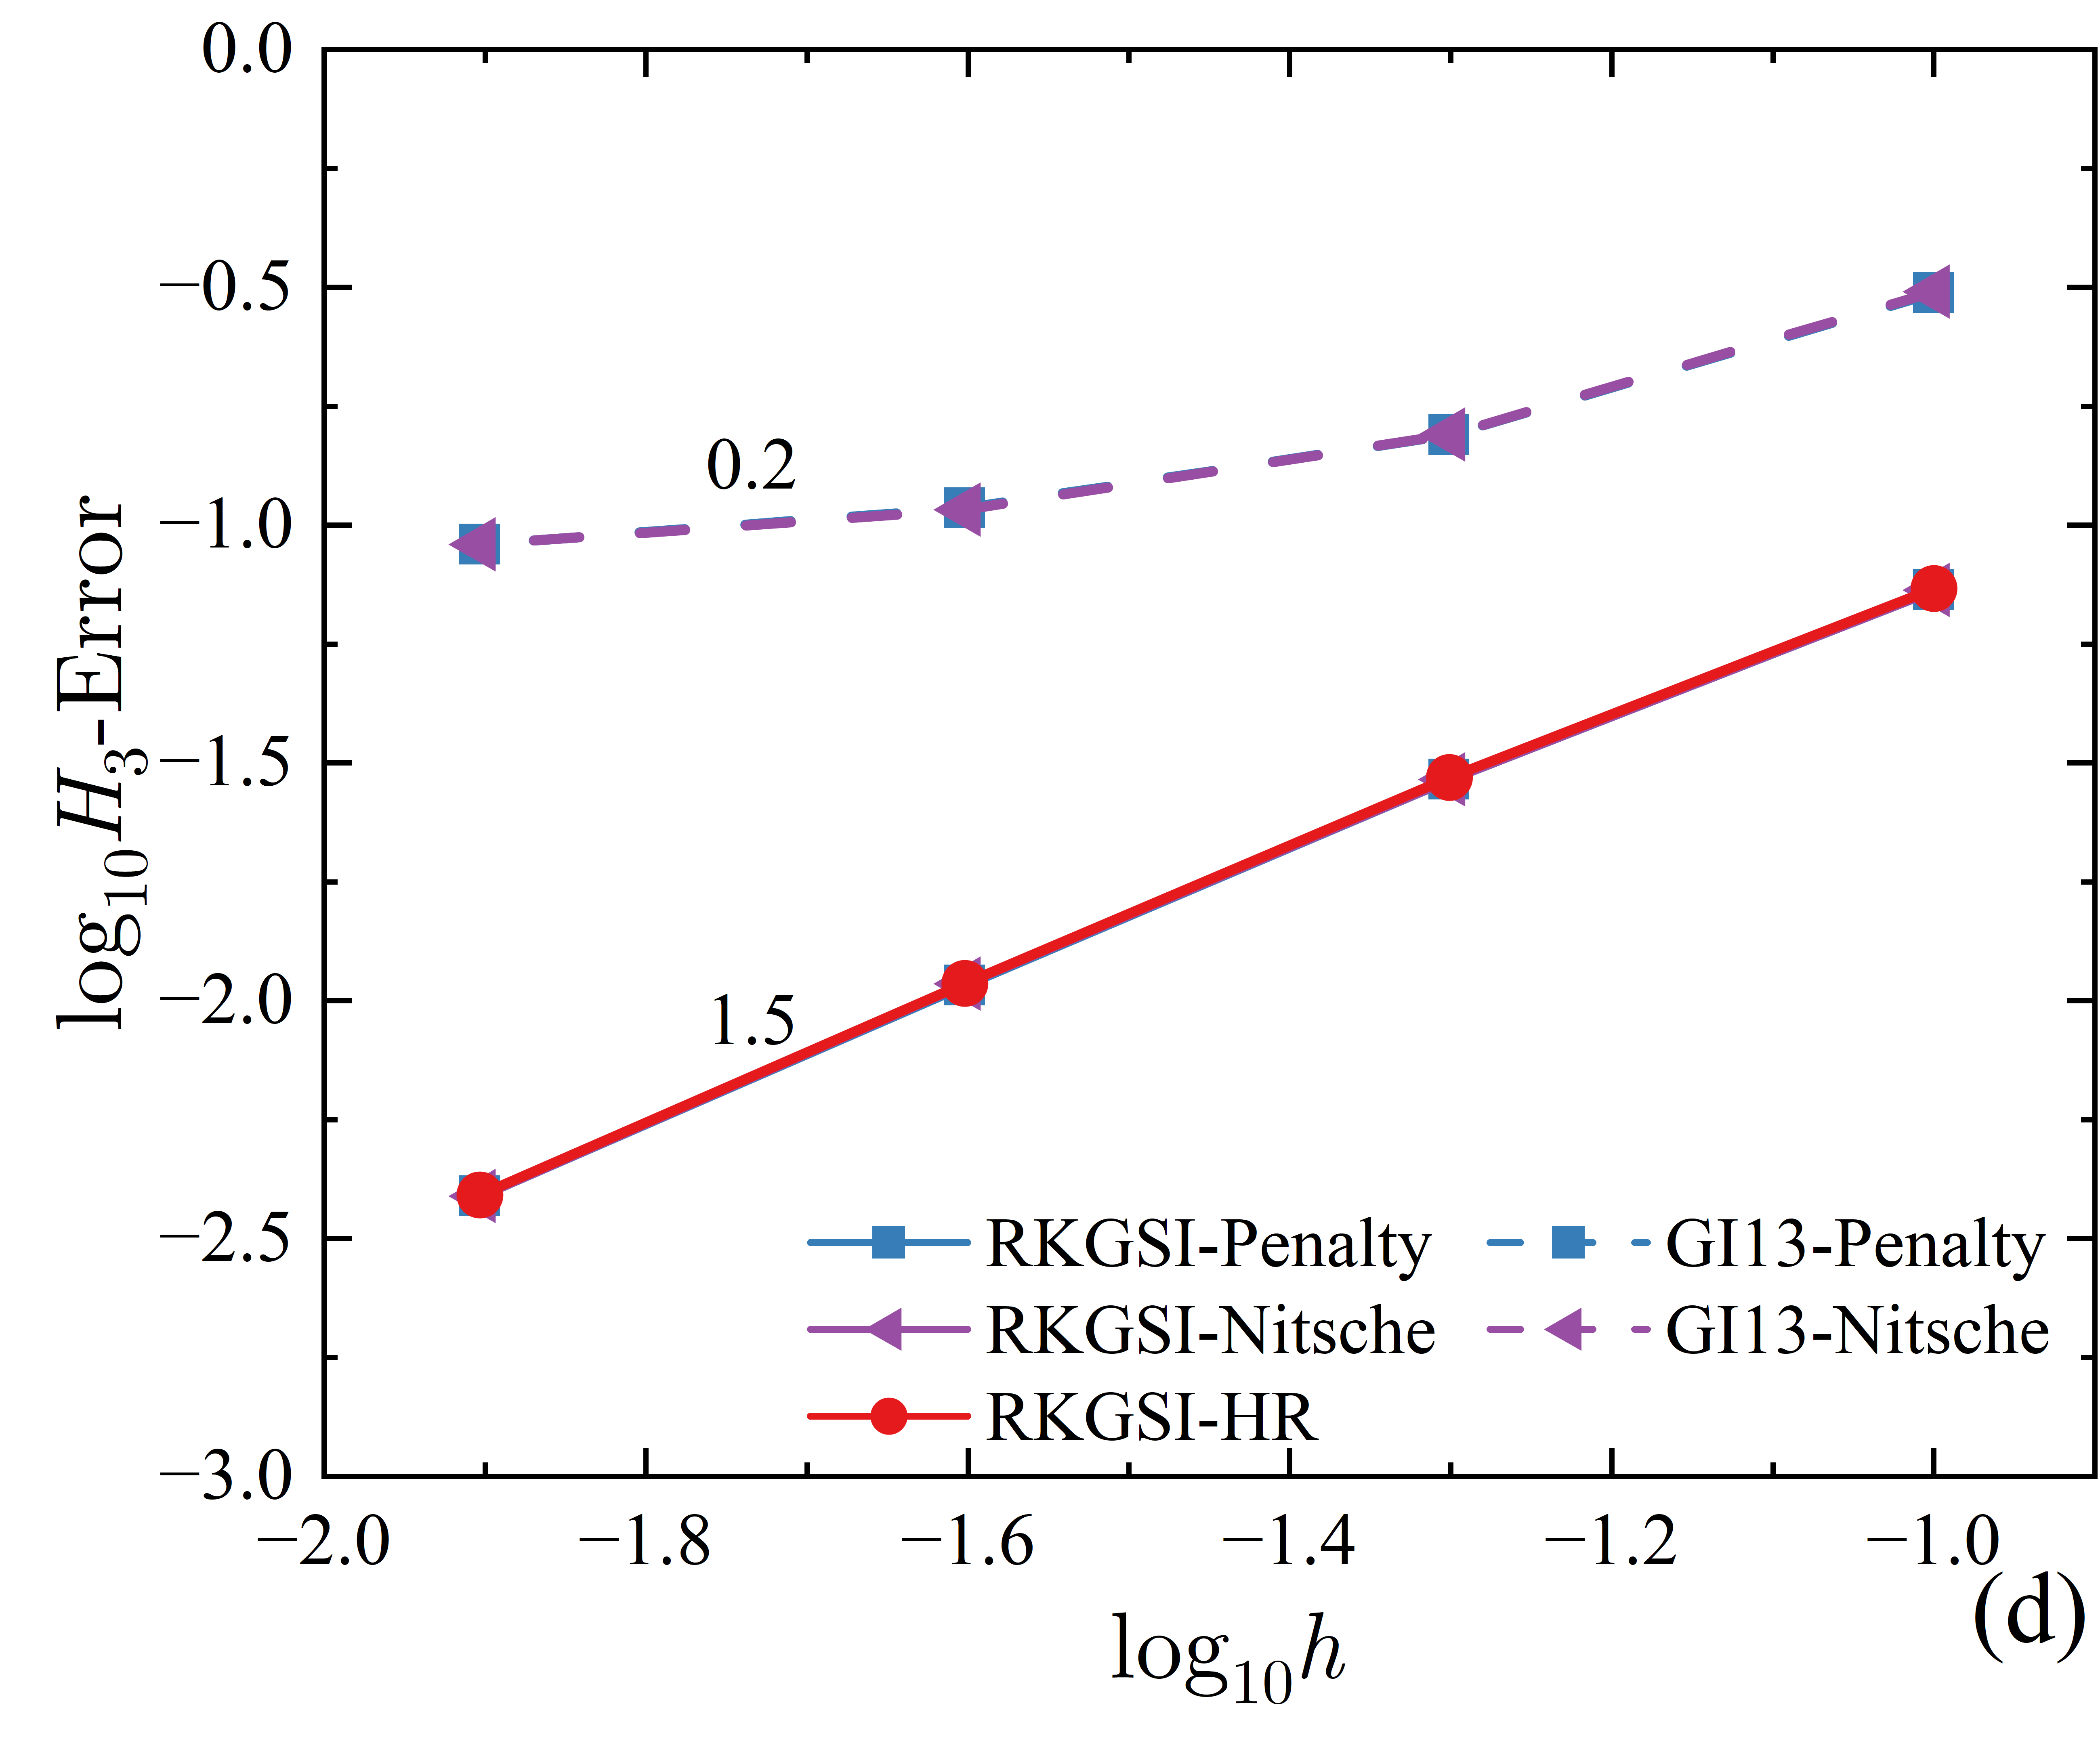
\includegraphics[width=0.49\textwidth]{figure/PHR/T/CH3.png}
    \phantomcaption\label{CH3}
    \end{subcaptiongroup}
\caption{简支等边三角形板问题三次基函数误差对比:\subref{CL2} $L_2$误差;\subref{CH1} $H_1$误差;\subref{CH2}$H_2$误差;\subref{CH3} $H_3$误差}
\label{TCLH}
\end{figure}
\begin{figure}[H]
    \centering
    \begin{subcaptiongroup}
    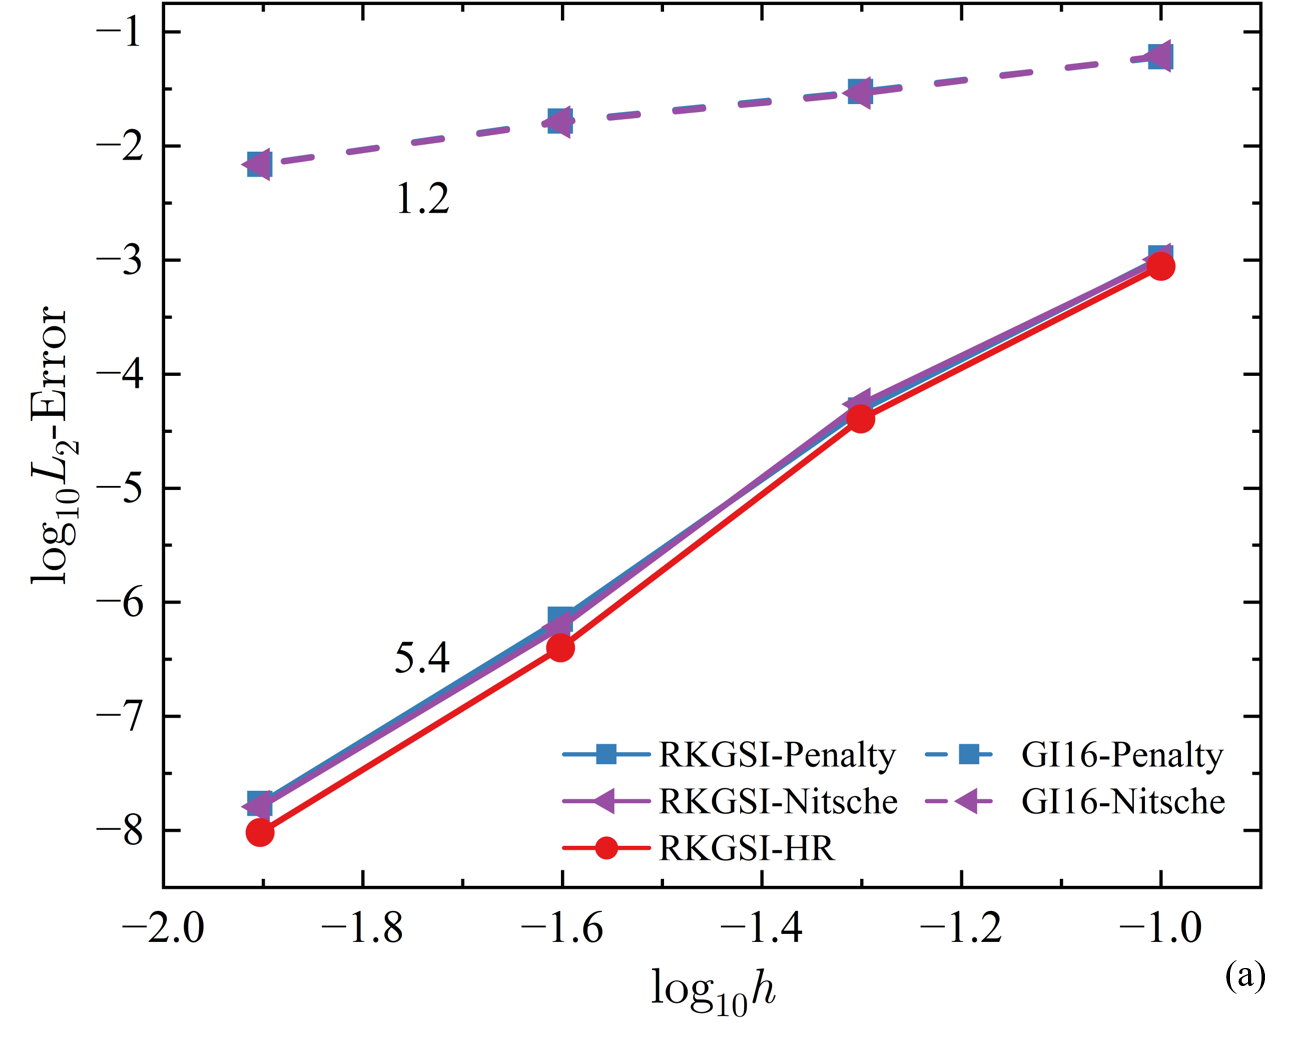
\includegraphics[width=0.49\textwidth]{figure/PHR/T/QL2.png}
    \phantomcaption\label{QL2}
    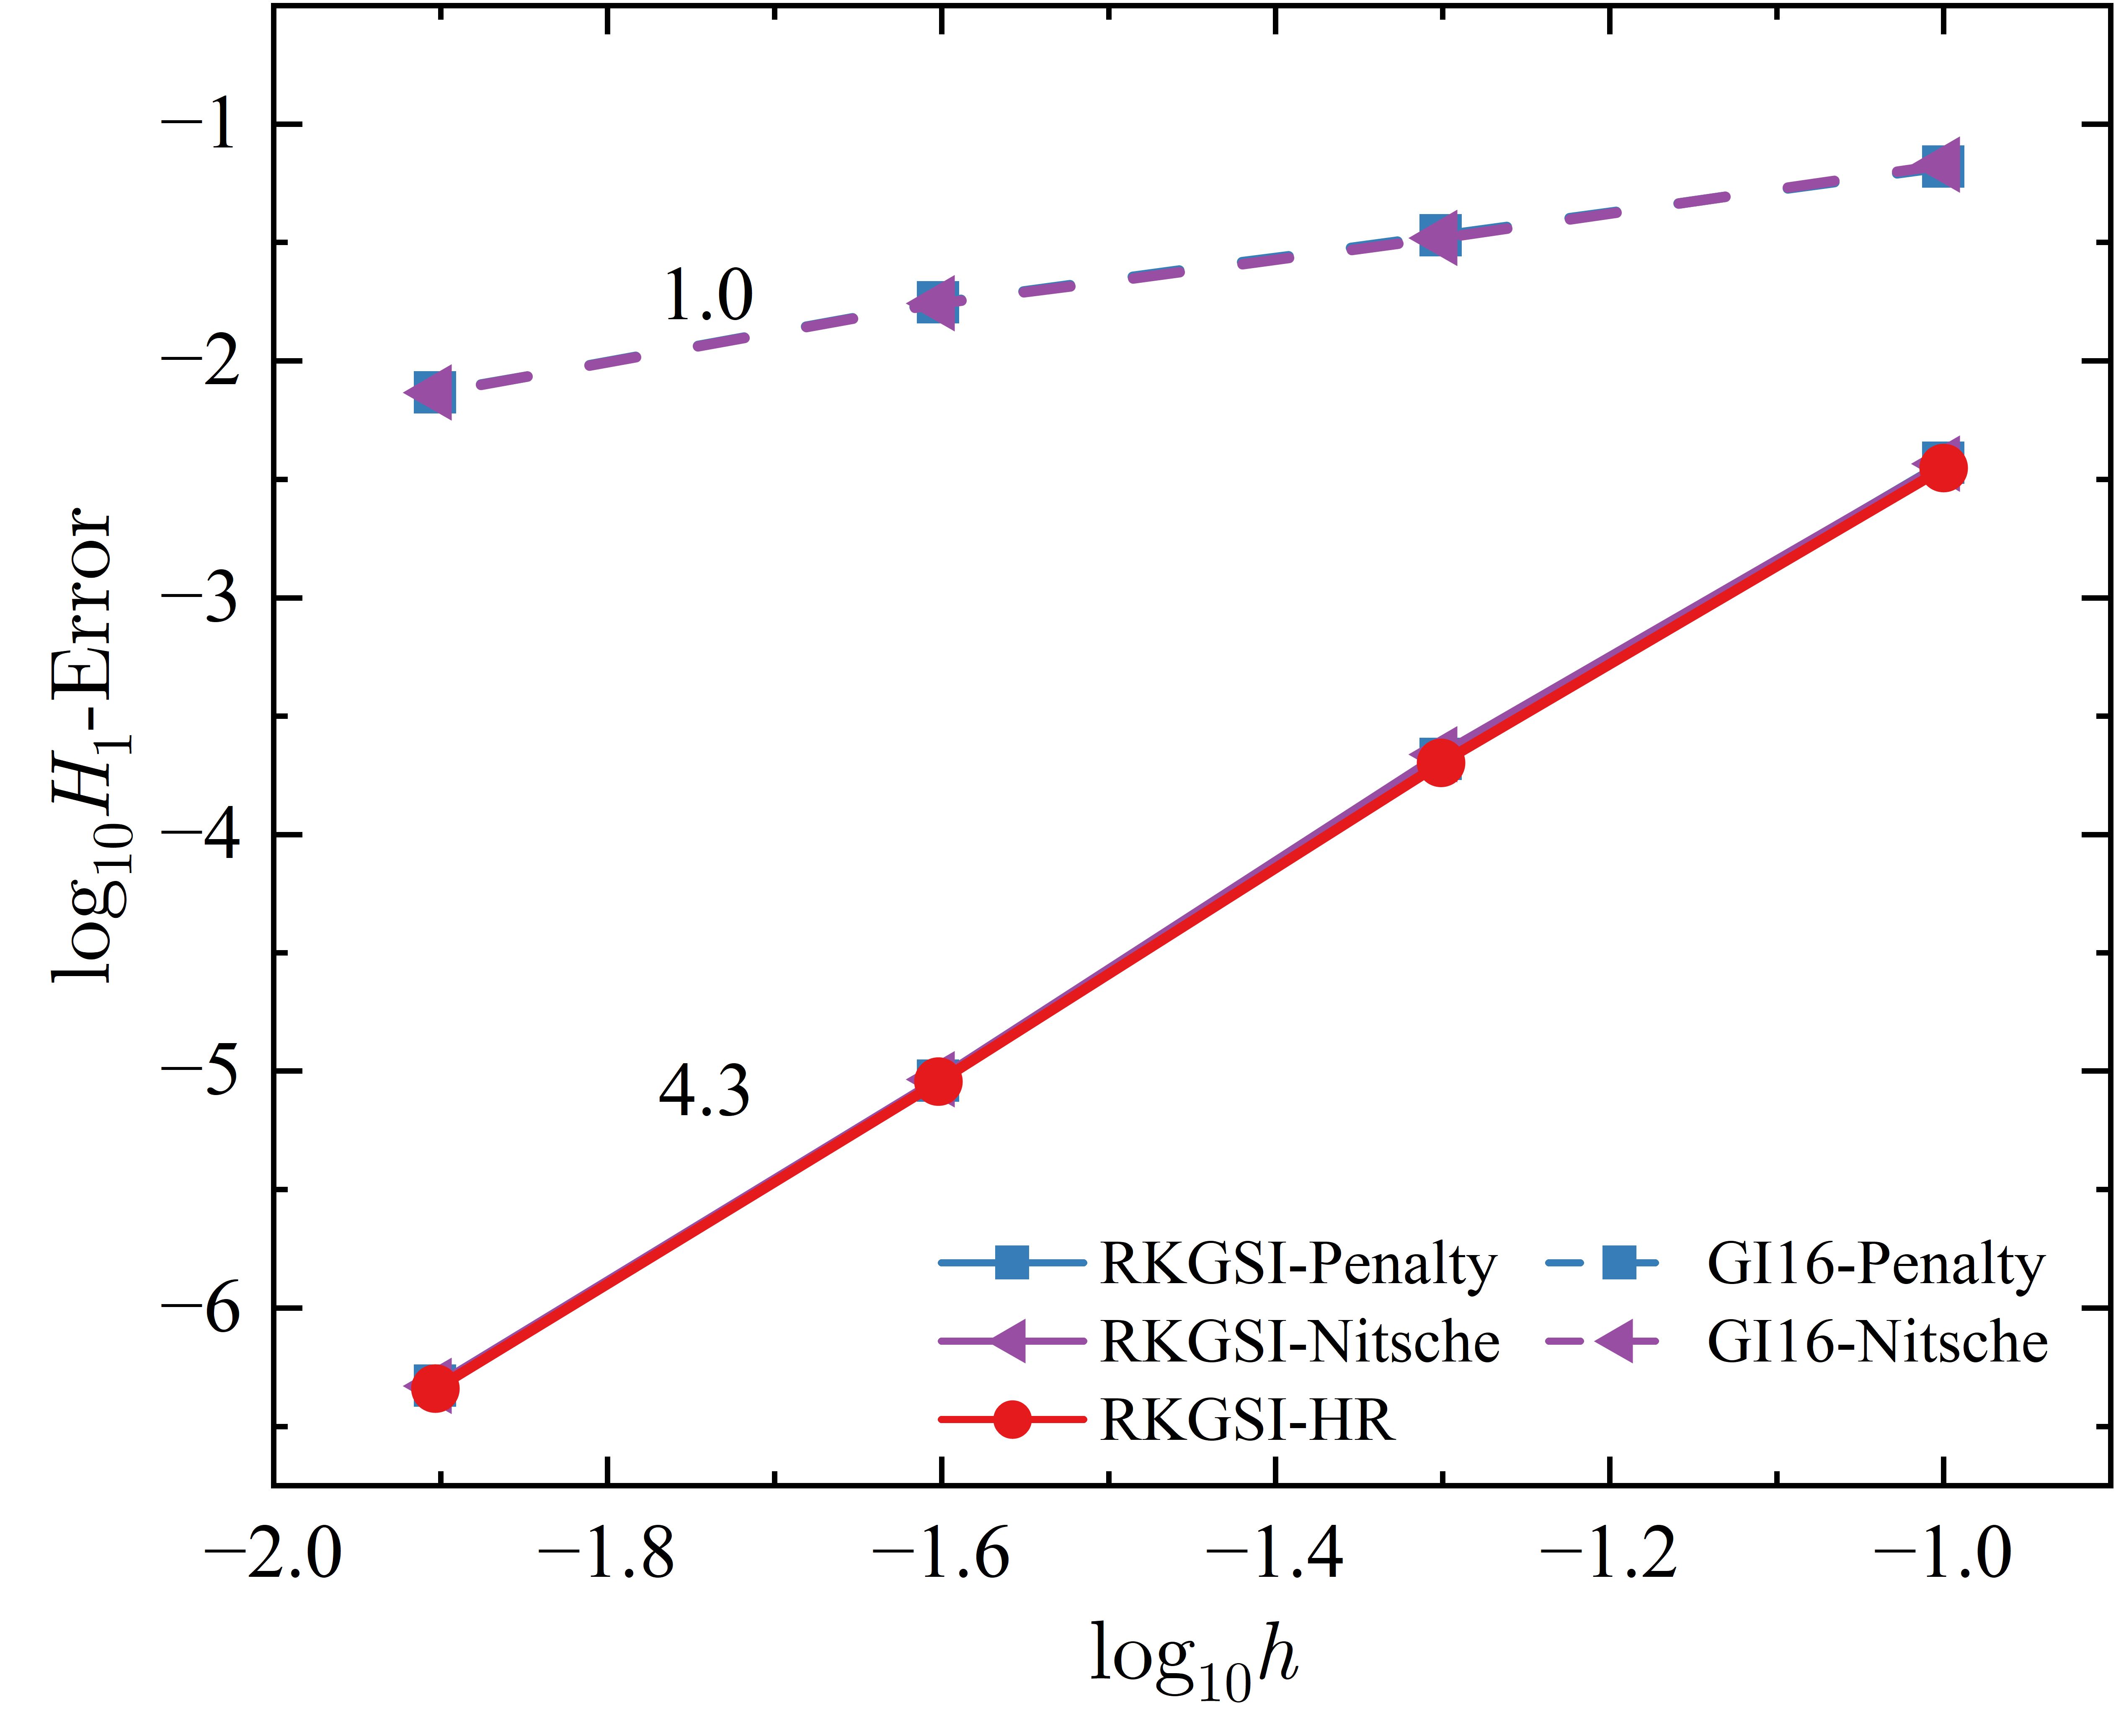
\includegraphics[width=0.49\textwidth]{figure/PHR/T/QH1.png}
    \phantomcaption\label{QH1}
    \end{subcaptiongroup}
    \begin{subcaptiongroup}
    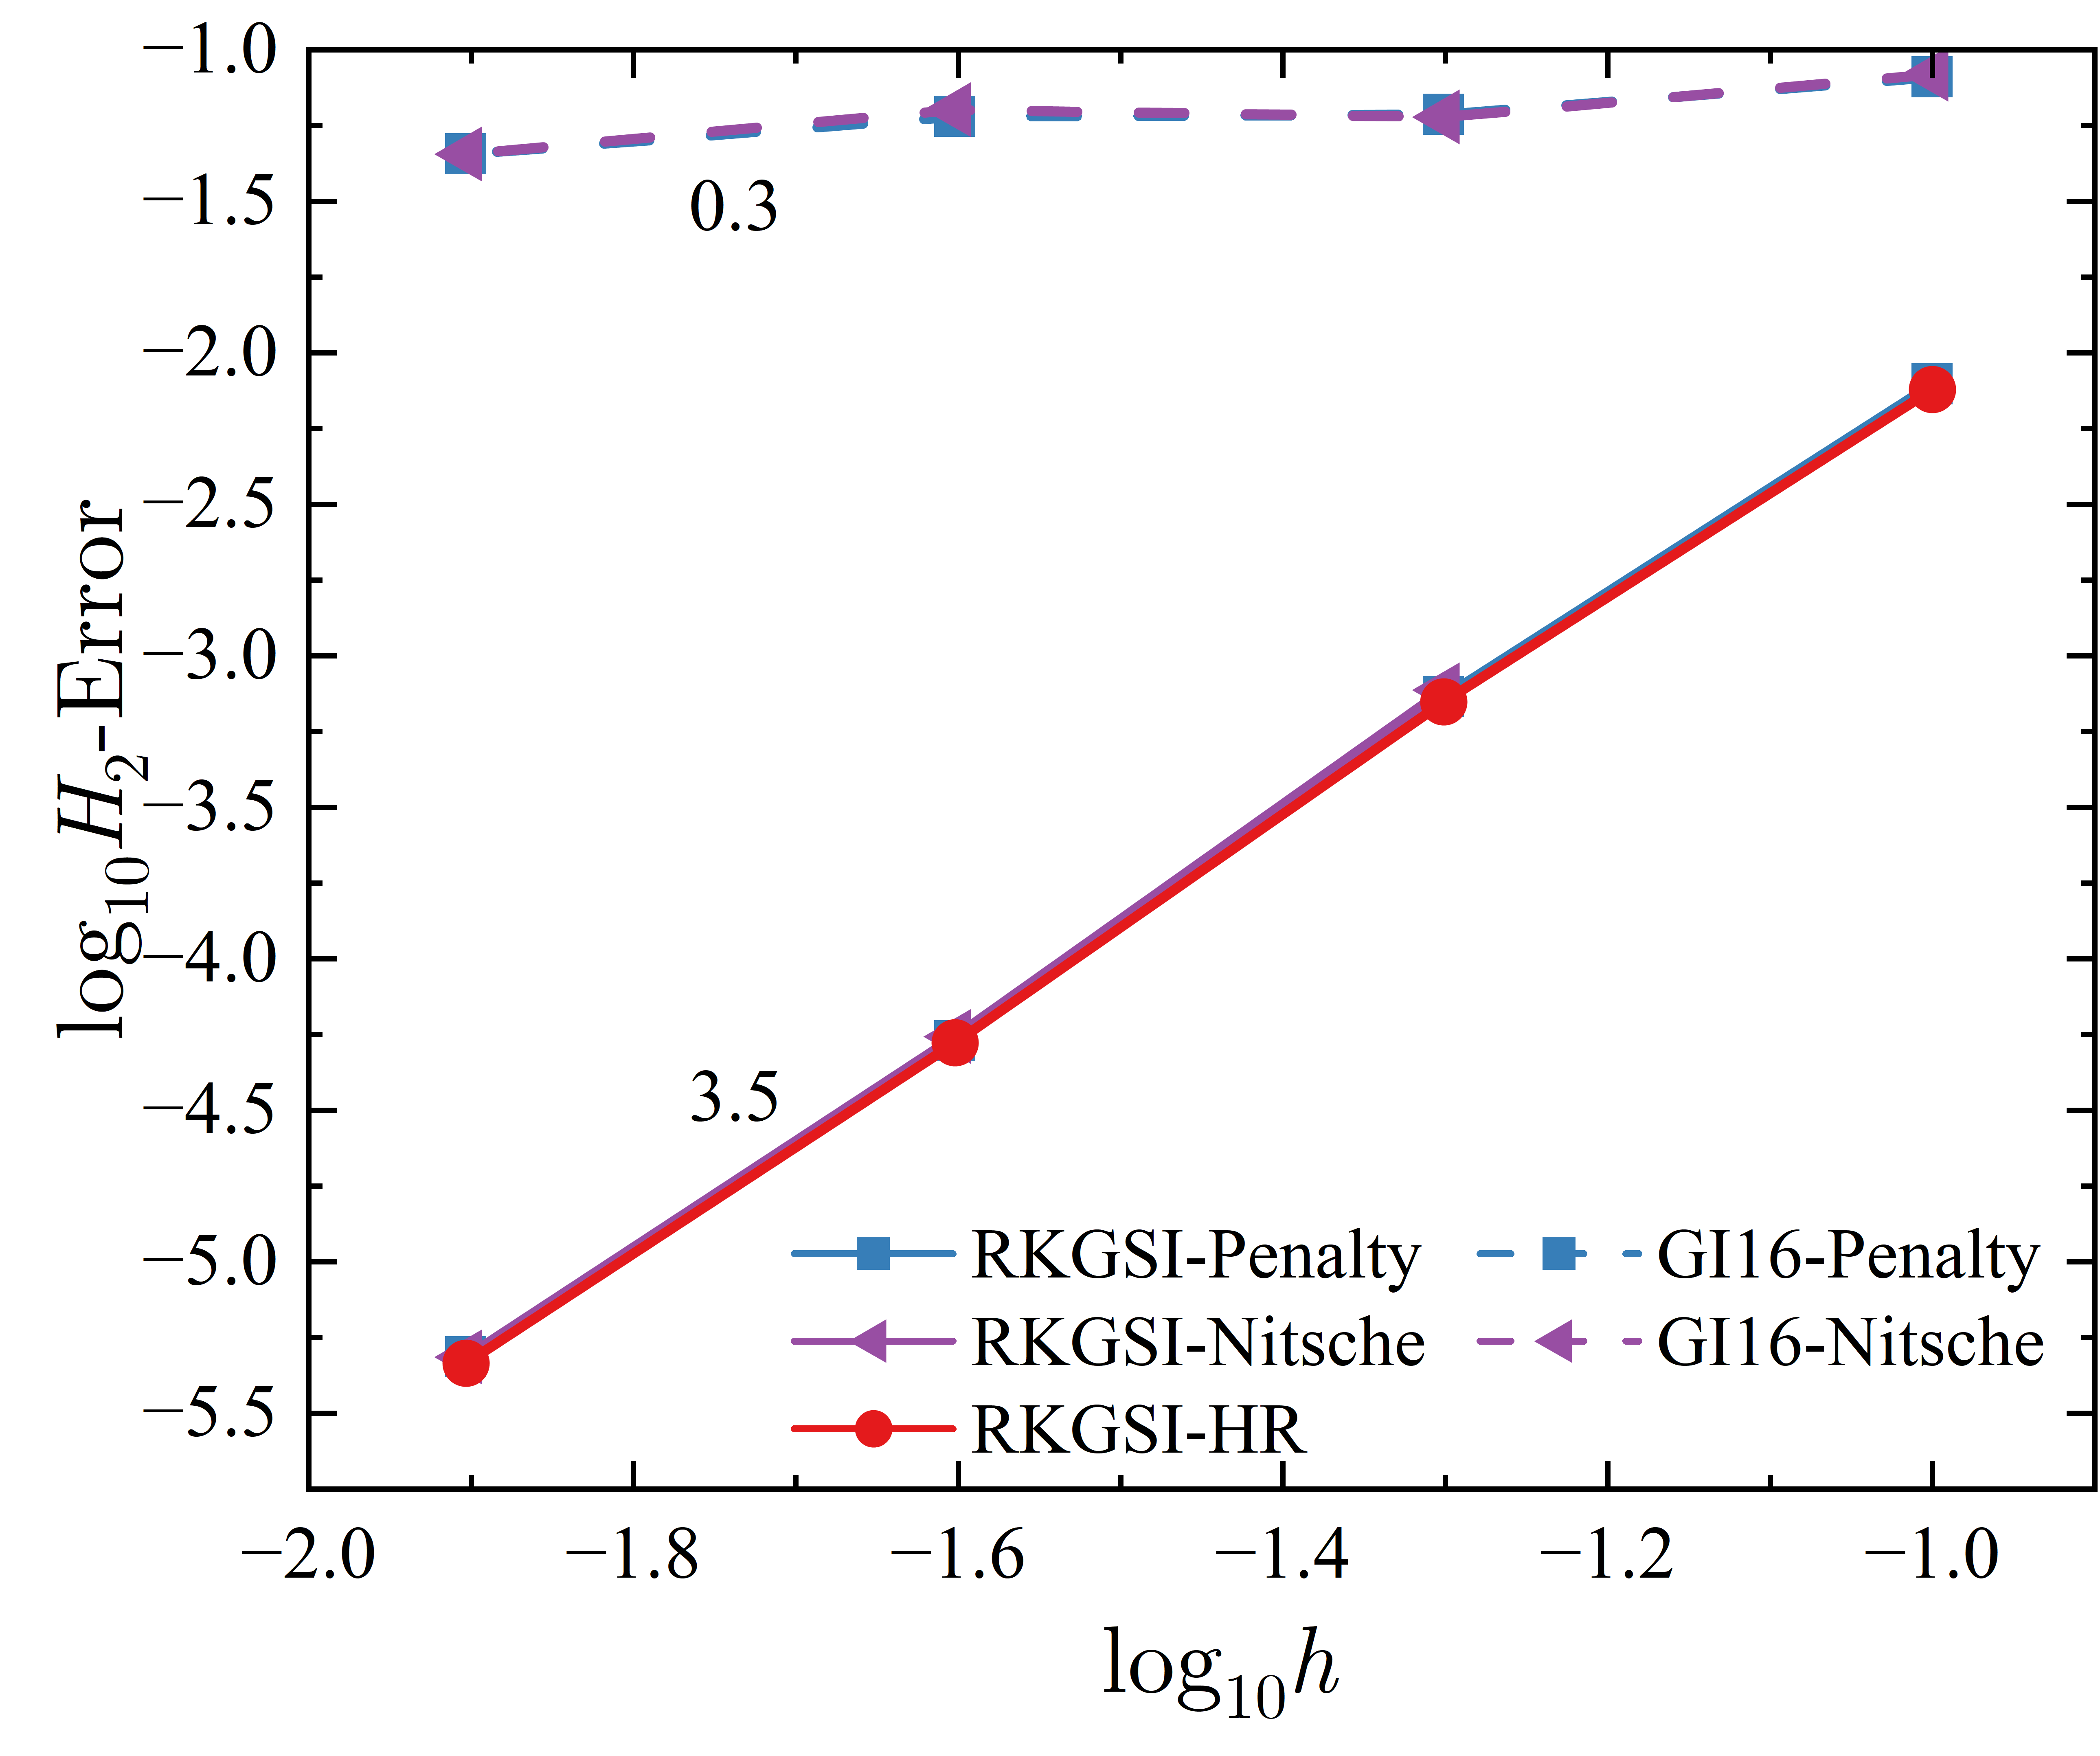
\includegraphics[width=0.49\textwidth]{figure/PHR/T/QH2.png}
    \phantomcaption\label{QH2}
    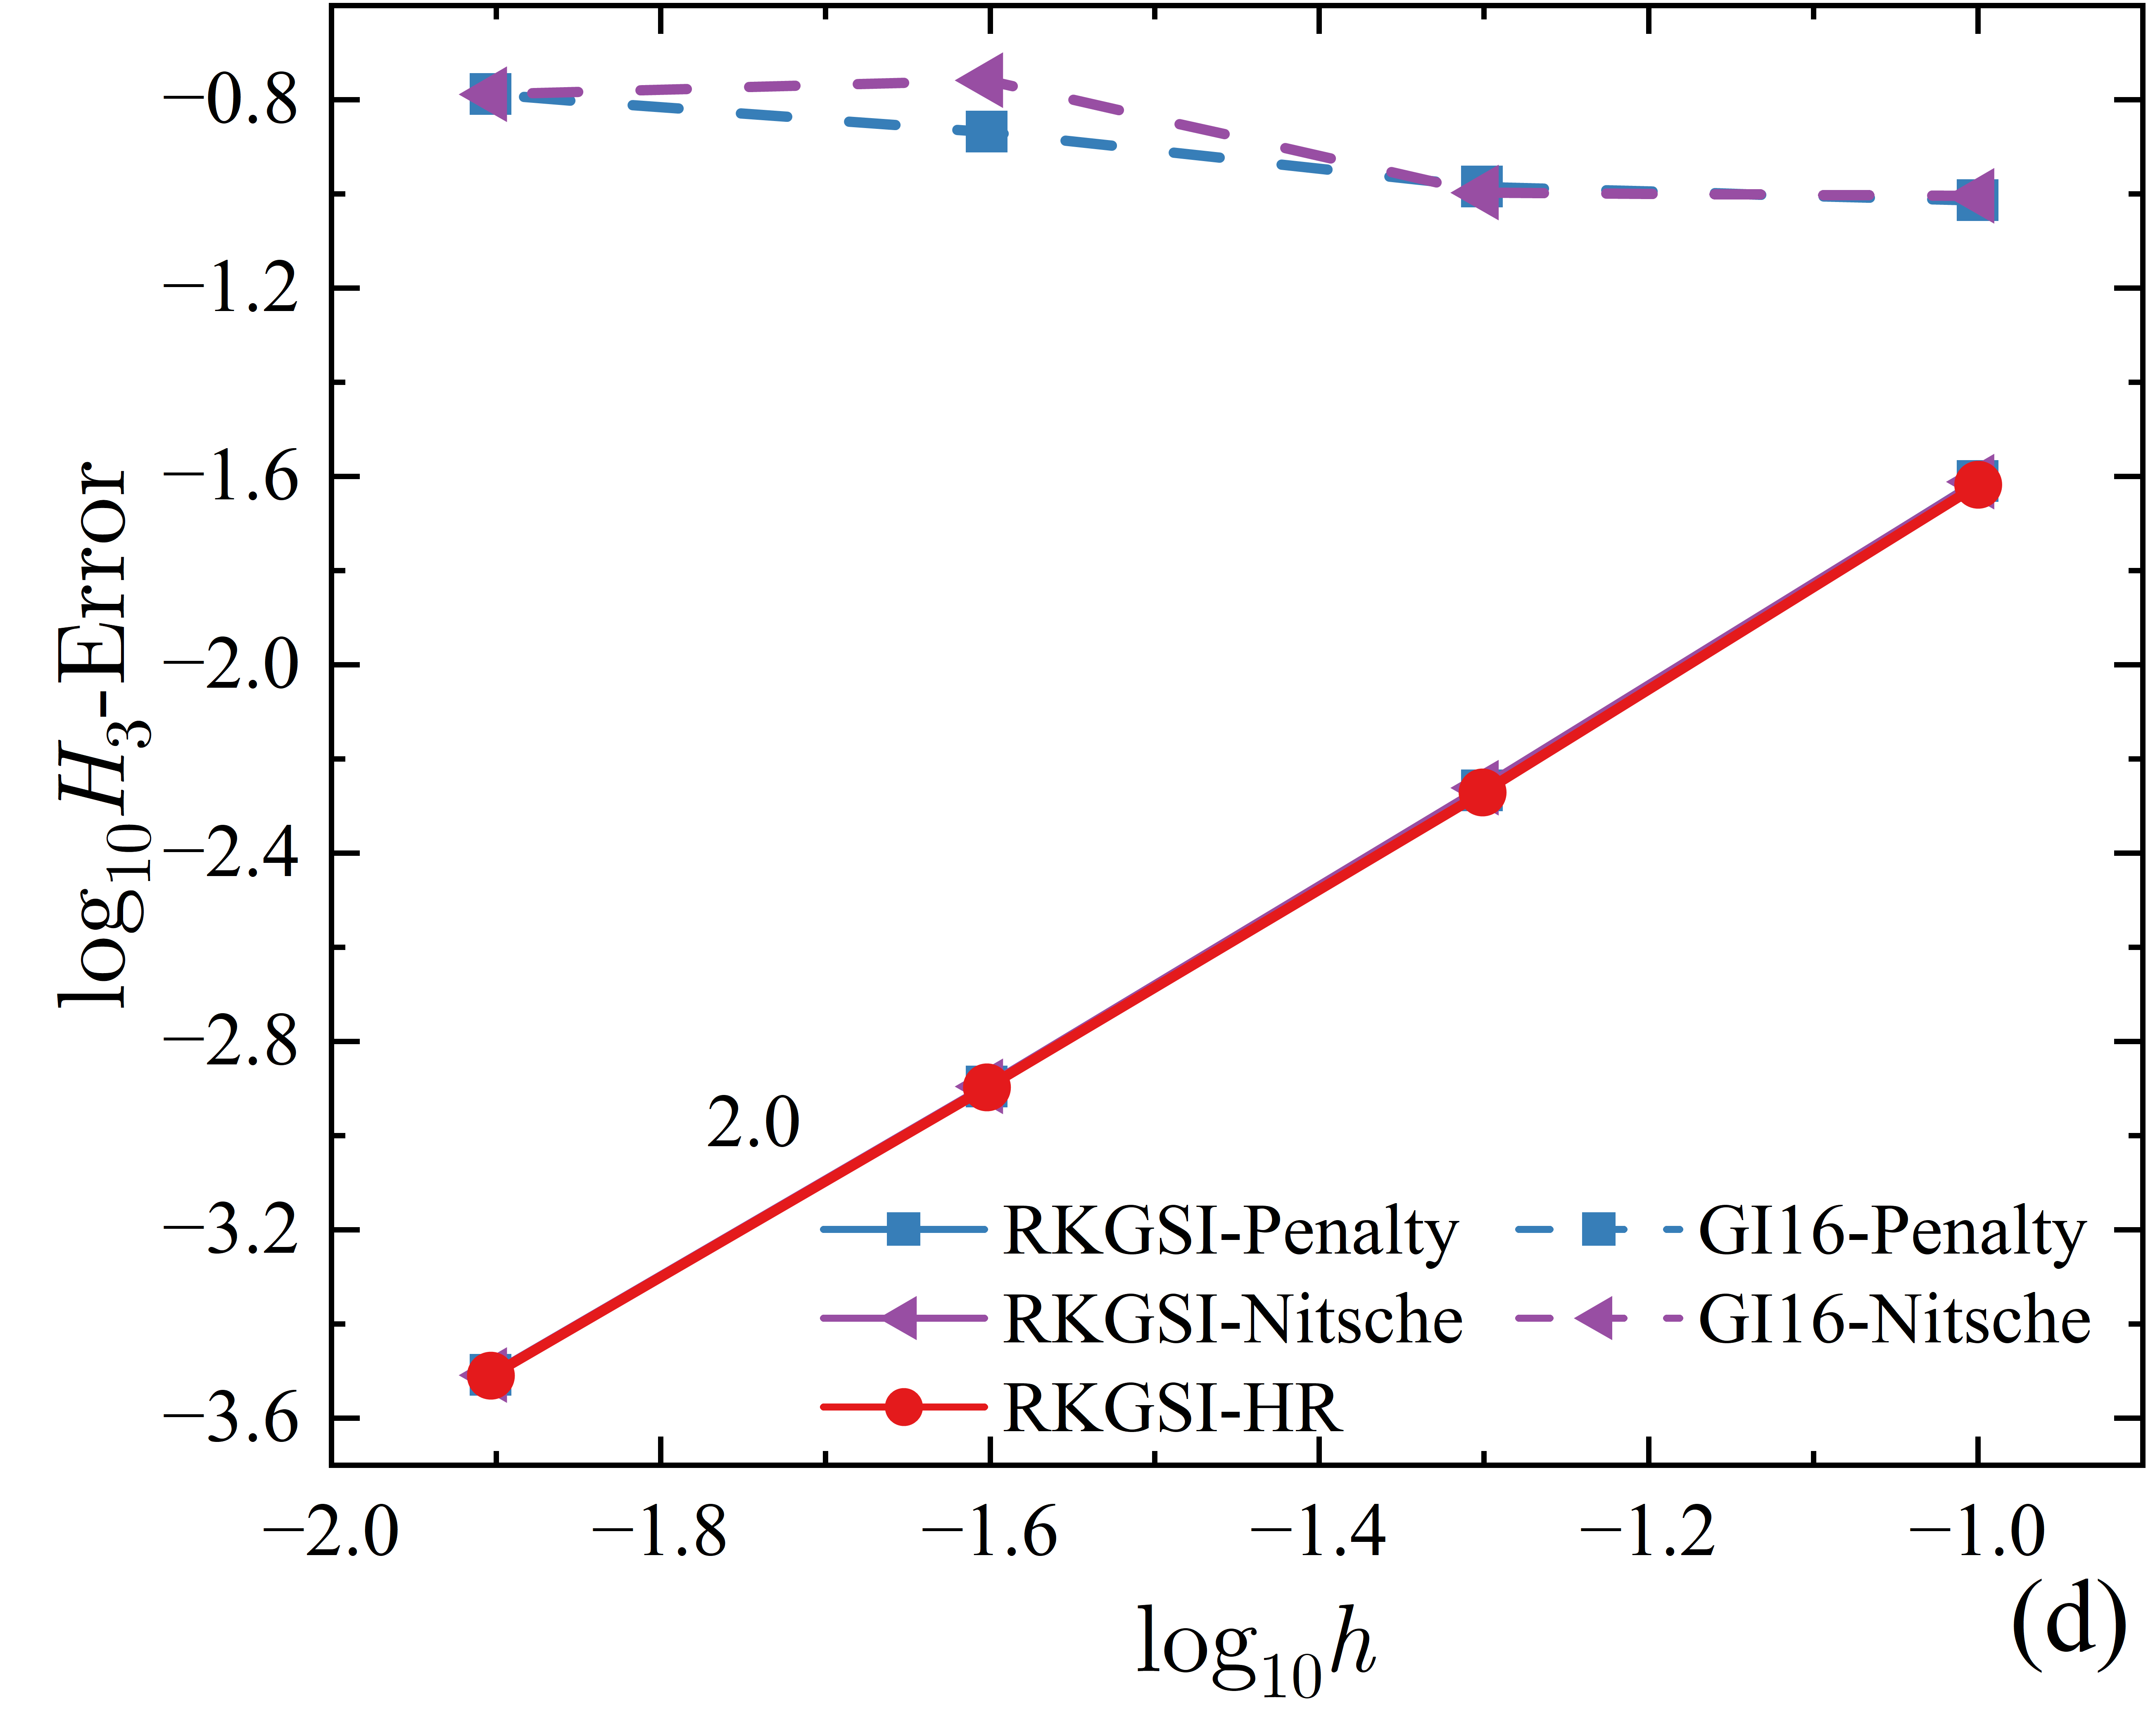
\includegraphics[width=0.49\textwidth]{figure/PHR/T/QH3.png}
    \phantomcaption\label{QH3}
    \end{subcaptiongroup}
\caption{简支等边三角形板问题四次基函数误差对比:\subref{QL2} $L_2$误差;\subref{QH1} $H_1$;误差\subref{QH2};$H_2$误差;\subref{QH3} $H_3$误差}
\label{TQLH}
\end{figure}
\begin{figure}[H]
    \centering
    \begin{subcaptiongroup}
    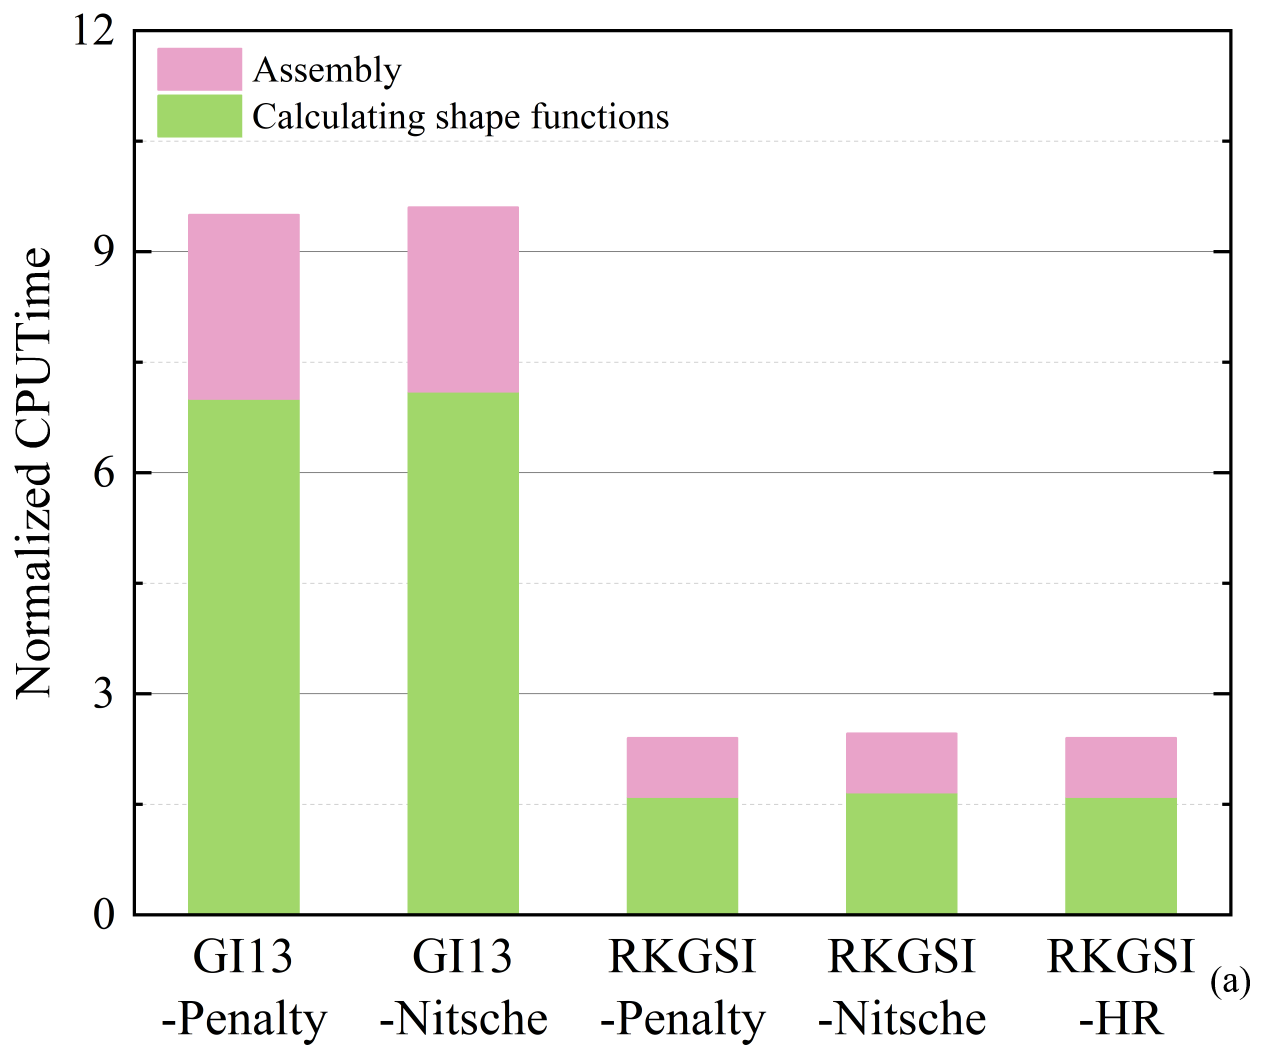
\includegraphics[width=0.49\textwidth]{figure/PHR/T/Cefficiencyomega.png}
    \phantomcaption\label{Cefficiencyomega}
    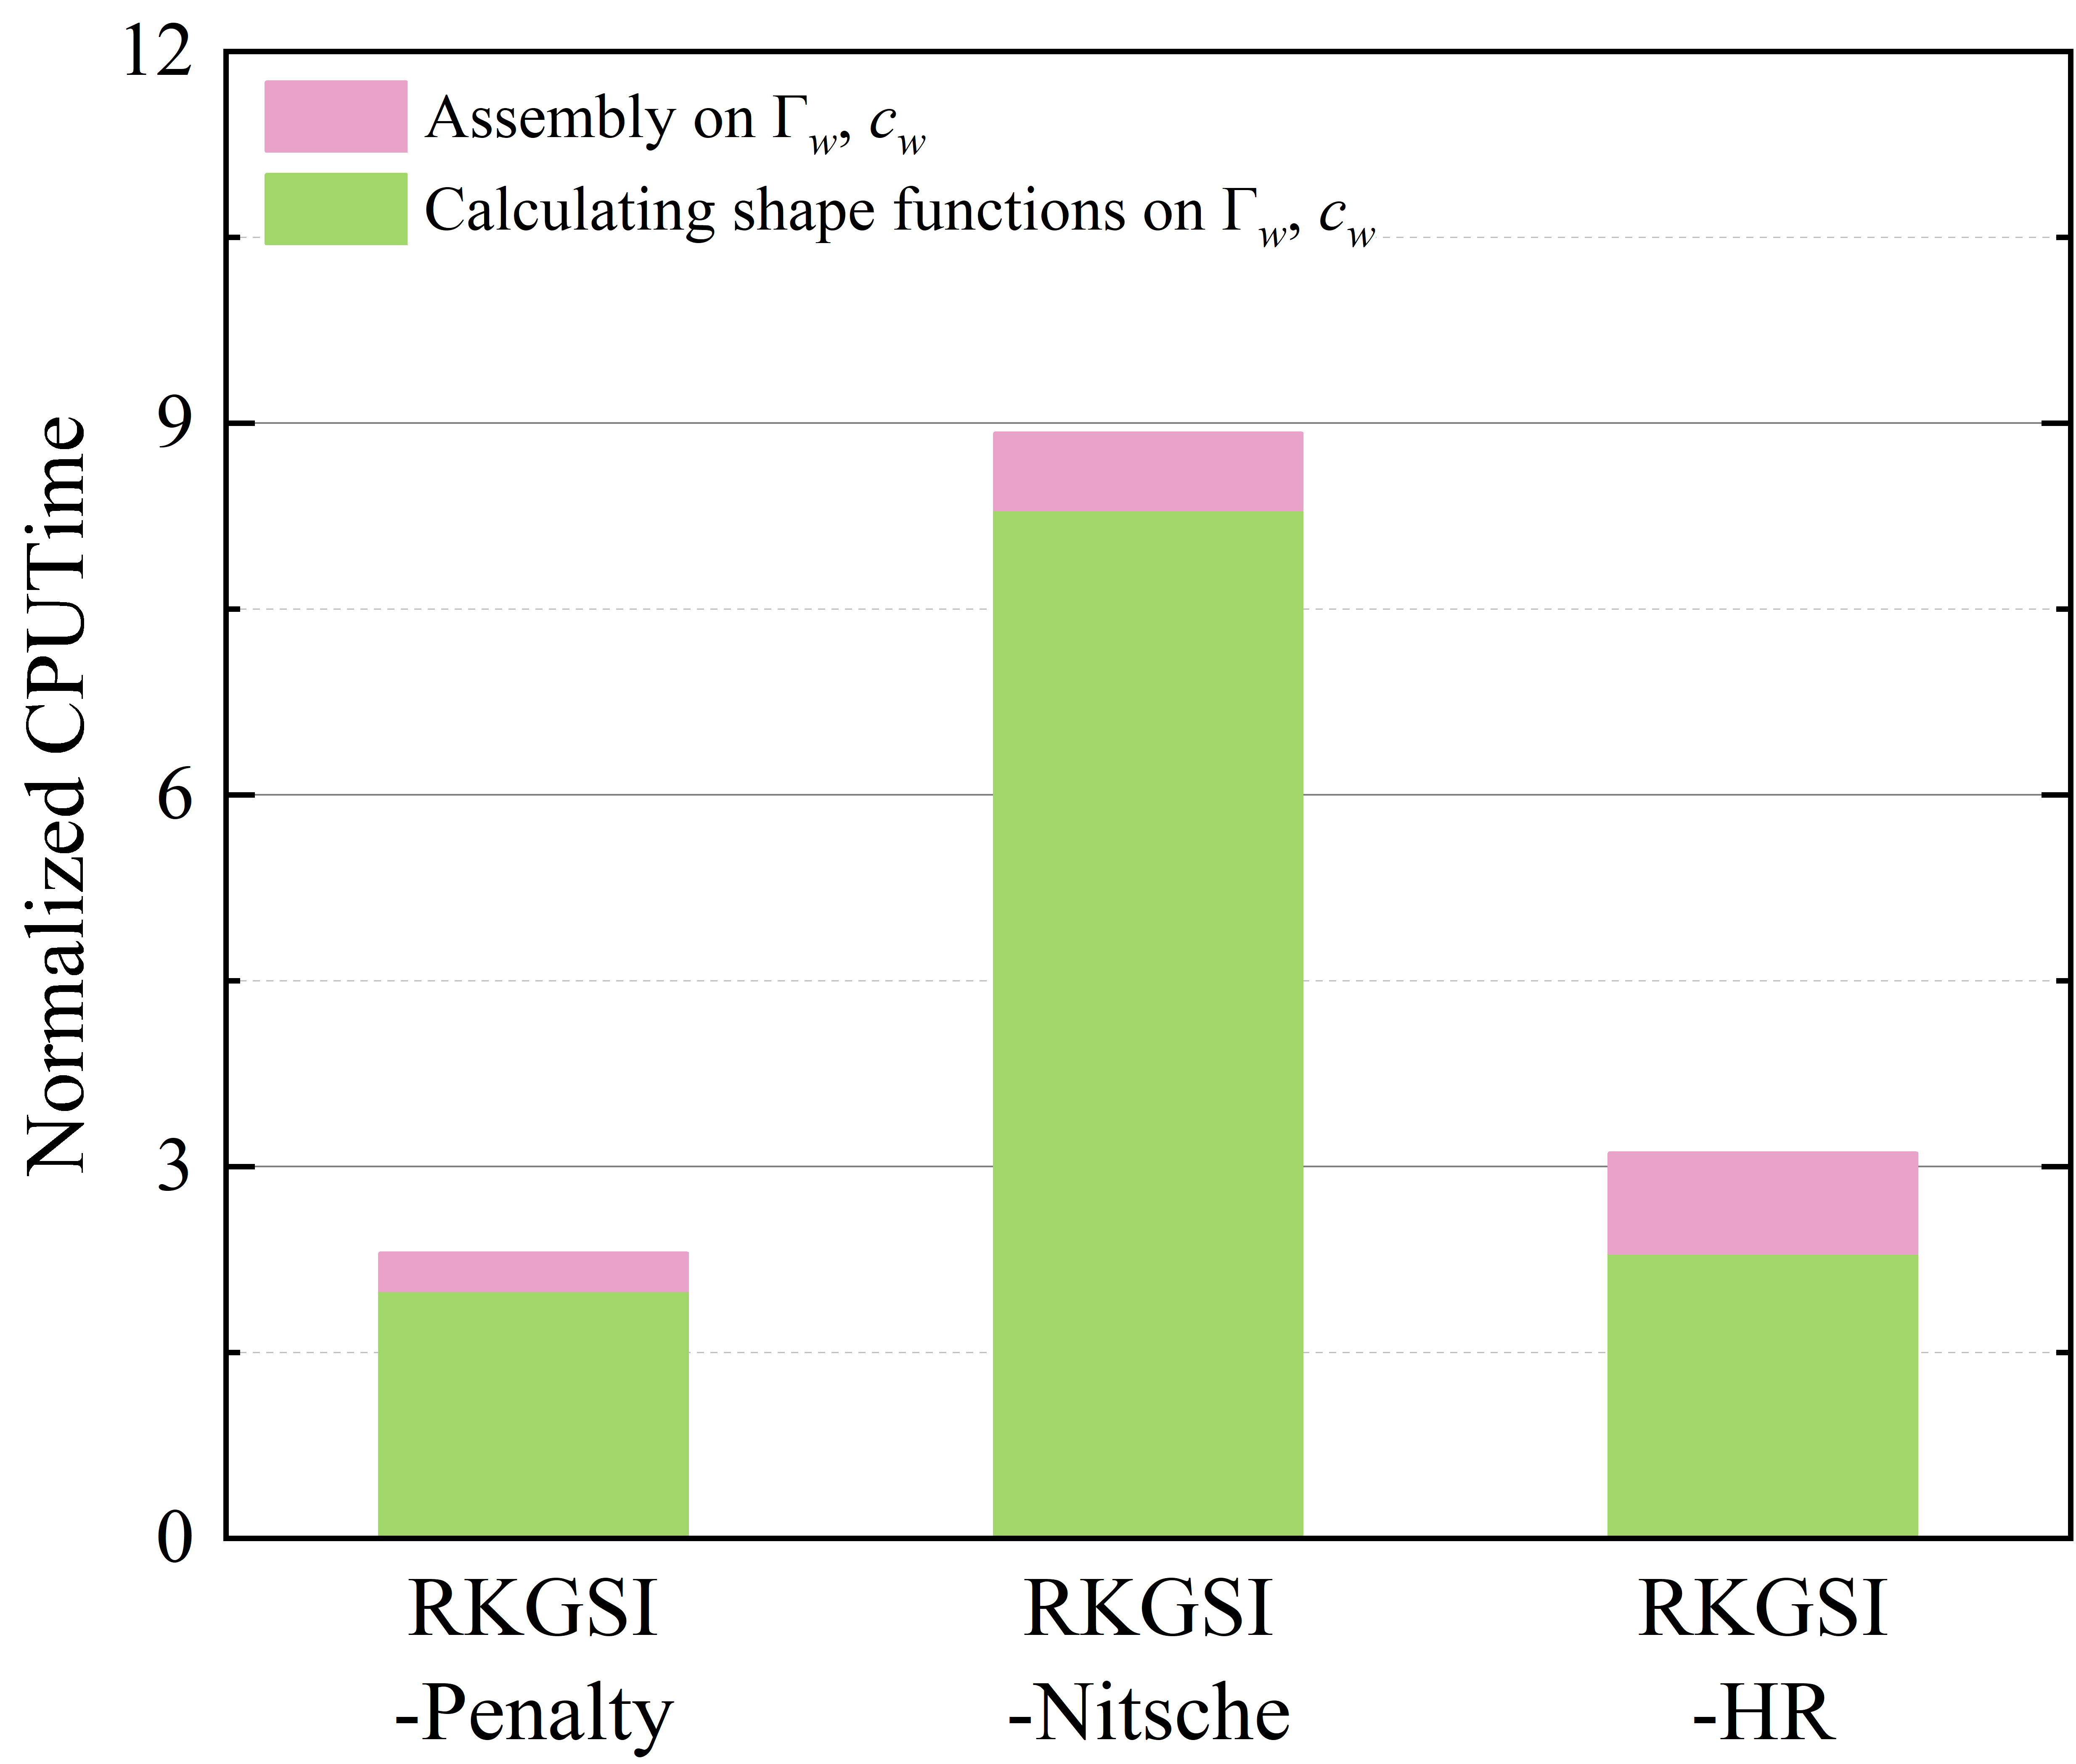
\includegraphics[width=0.49\textwidth]{figure/PHR/T/Cefficiencygamma.png}
    \phantomcaption\label{Cefficiencygamma}
    \end{subcaptiongroup}
\caption{简支等边三角形问题效率对比:\subref{Cefficiencyomega}薄板中面$\Omega$;\subref{Cefficiencygamma}本质边界条件$\Gamma_w,c_w$}
\label{Tefficiency}
\end{figure}
\begin{figure}[H]
\centering
    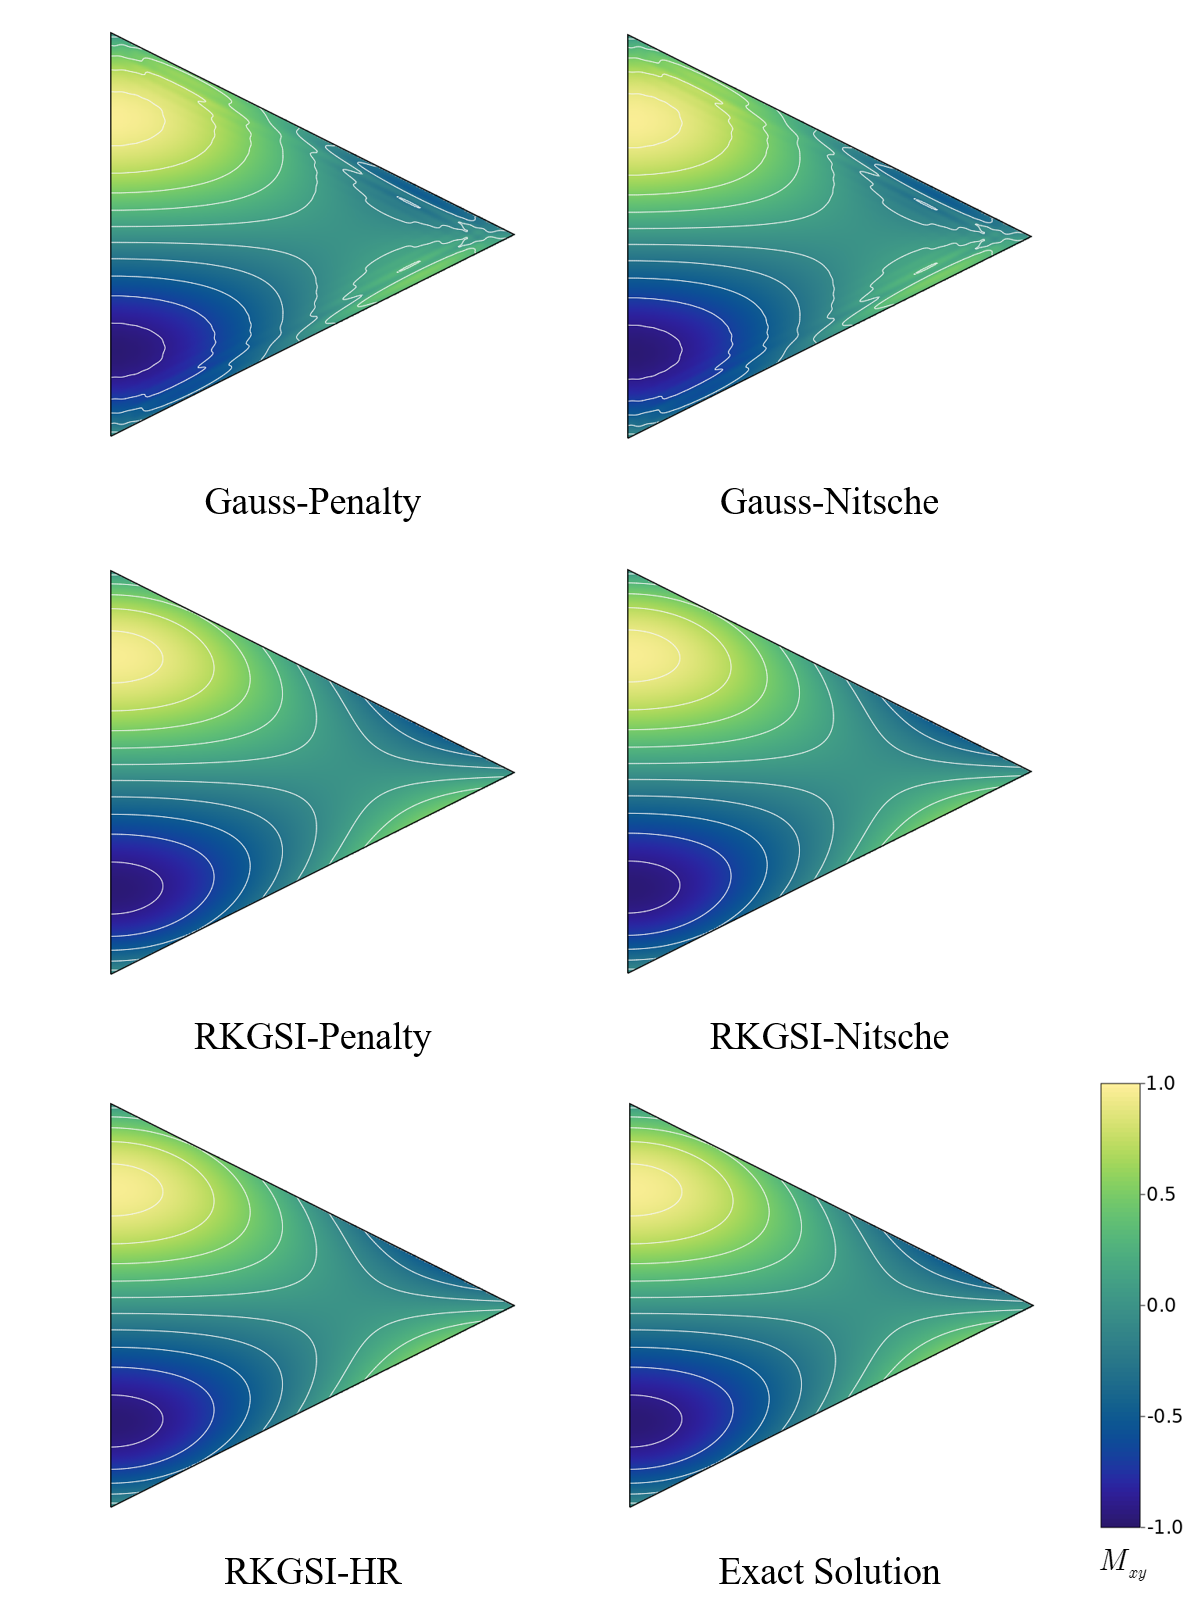
\includegraphics[scale=0.7]{figure/PHR/T/Mxy.png}
\caption{简支等边三角形板问题弯矩云图$\sigma_{xx}$应力云图}
\label{TMxy}
\end{figure}  
\subsection{简支环行板问题}
一简支环行板如图(\ref{annular})所示,其中内外径分别为$a=2$、$b=1$。在环行板的内外径边缘处分别施加弯矩$m_i=2$、$m_0=1$,
材料系数分别为抗弯刚度$\bar{D}=1$、泊松比为$\nu=0.3$。该简支环行板的精确解为:
\begin{equation}
\begin{split}
    w=\frac{(m_i-m_0)a^2b^2}{\bar D(1-\nu)(a^2-b^2)}ln\frac{r}{a}+\frac{m_ib^2-m_oa^2}{2\bar D(1+\nu)(a^2-b^2)}(r^2-a^2)
\end{split}
\end{equation}
其中:$r=\sqrt{x^2+y^2}$是点($x,y$)的极径。
\begin{figure}[H]
    \centering
    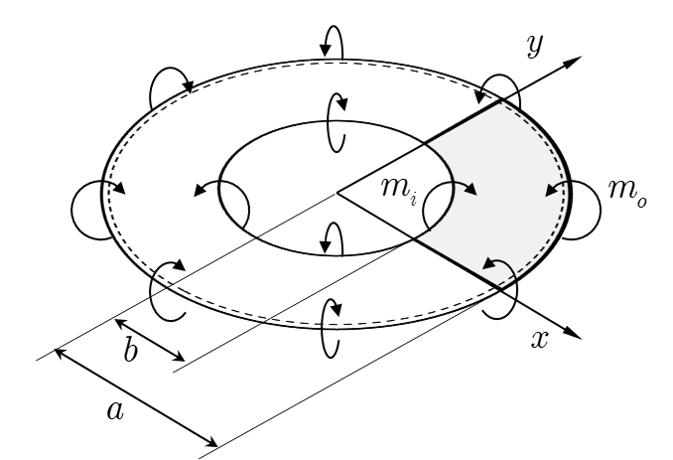
\includegraphics[scale=0.7]{figure/PHR/A/annular.png}
    \caption{简支环形板问题模型}\label{annular}
\end{figure}
如图(\ref{annularmsh})所示,简支环形问题求解域通过采用均布的153、561、2145和8385四个疏密不同的节点进行离散,
该简支环行板采用四次基函数,取相对影响域为4.5进行数值分析。\par
\begin{figure}[H]
    \centering
    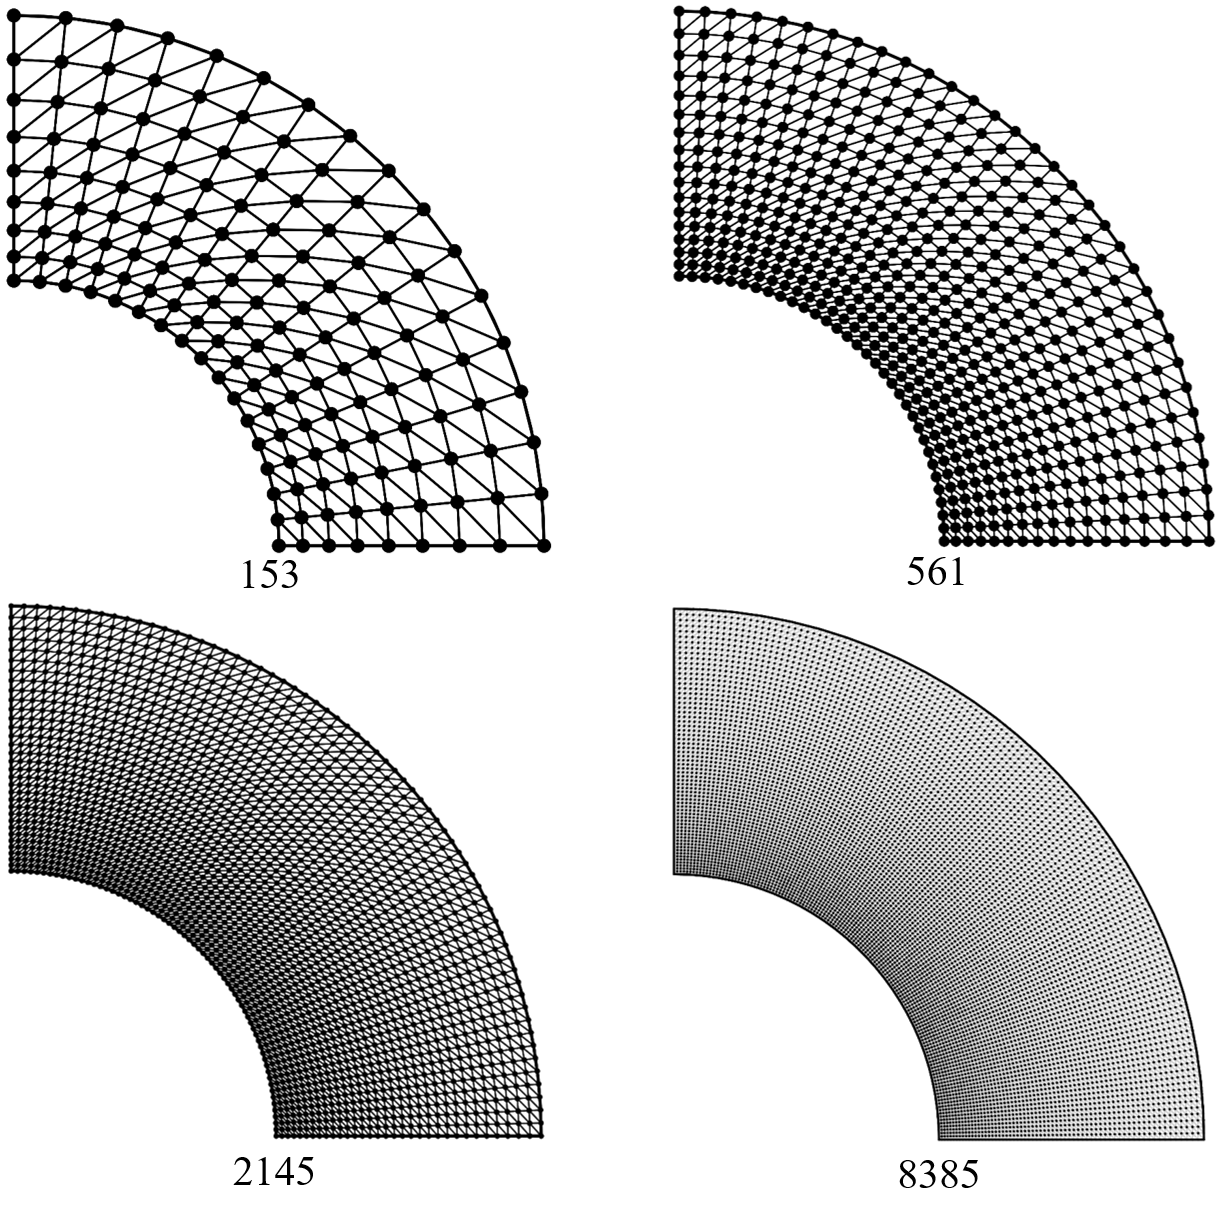
\includegraphics[scale=0.4]{figure/PHR/A/annularmsh.png}
    \caption{简支环形板问题节点离散}\label{annularmsh}
\end{figure}
图(\ref{AQLH})为简支环行板问题的位移误差和能量误差对比图,从图中可以看出“RKGSI-HR”和“RKGSI-Nitsche”同样可以达到理论误差收敛率。
图(\ref{AQcputime})为简支环行板问题在计算时间节点数和施加不同本质边界条件上的效率对比,从图中可以看出采用“RKGSI”时的效率明显高于“GI”法,
与同样满足变分一致性的“RKGSI-Nitsche”法相比,“RKGSI-HR”法在施加过程中效率明显更高。
同样根据简支环行板的弯矩云图(\ref{AMxy})也可以更进一步说明在解决薄板问题上,基于Hellinger-Reissner变分原理的本质边界条件施加方法拥有着更高的计算精度。
在简支环行板问题中,存在两个人工参数影响计算精度。从图(\ref{Aalpha})中可以看出,随着节点数的变化“RKGSI-Nitsche”法和“RKGSI-Penalty”法在达到最优精度时的人工参数值也在发生变化。
而“RKGSI-HR”法中不涉及人工参数,因此随着节点数的增加,计算精度不会受到人工参数的影响,从而提高了一种更稳定和高效的计算方法。
\begin{figure}[H]
    \centering
    \begin{subcaptiongroup}
    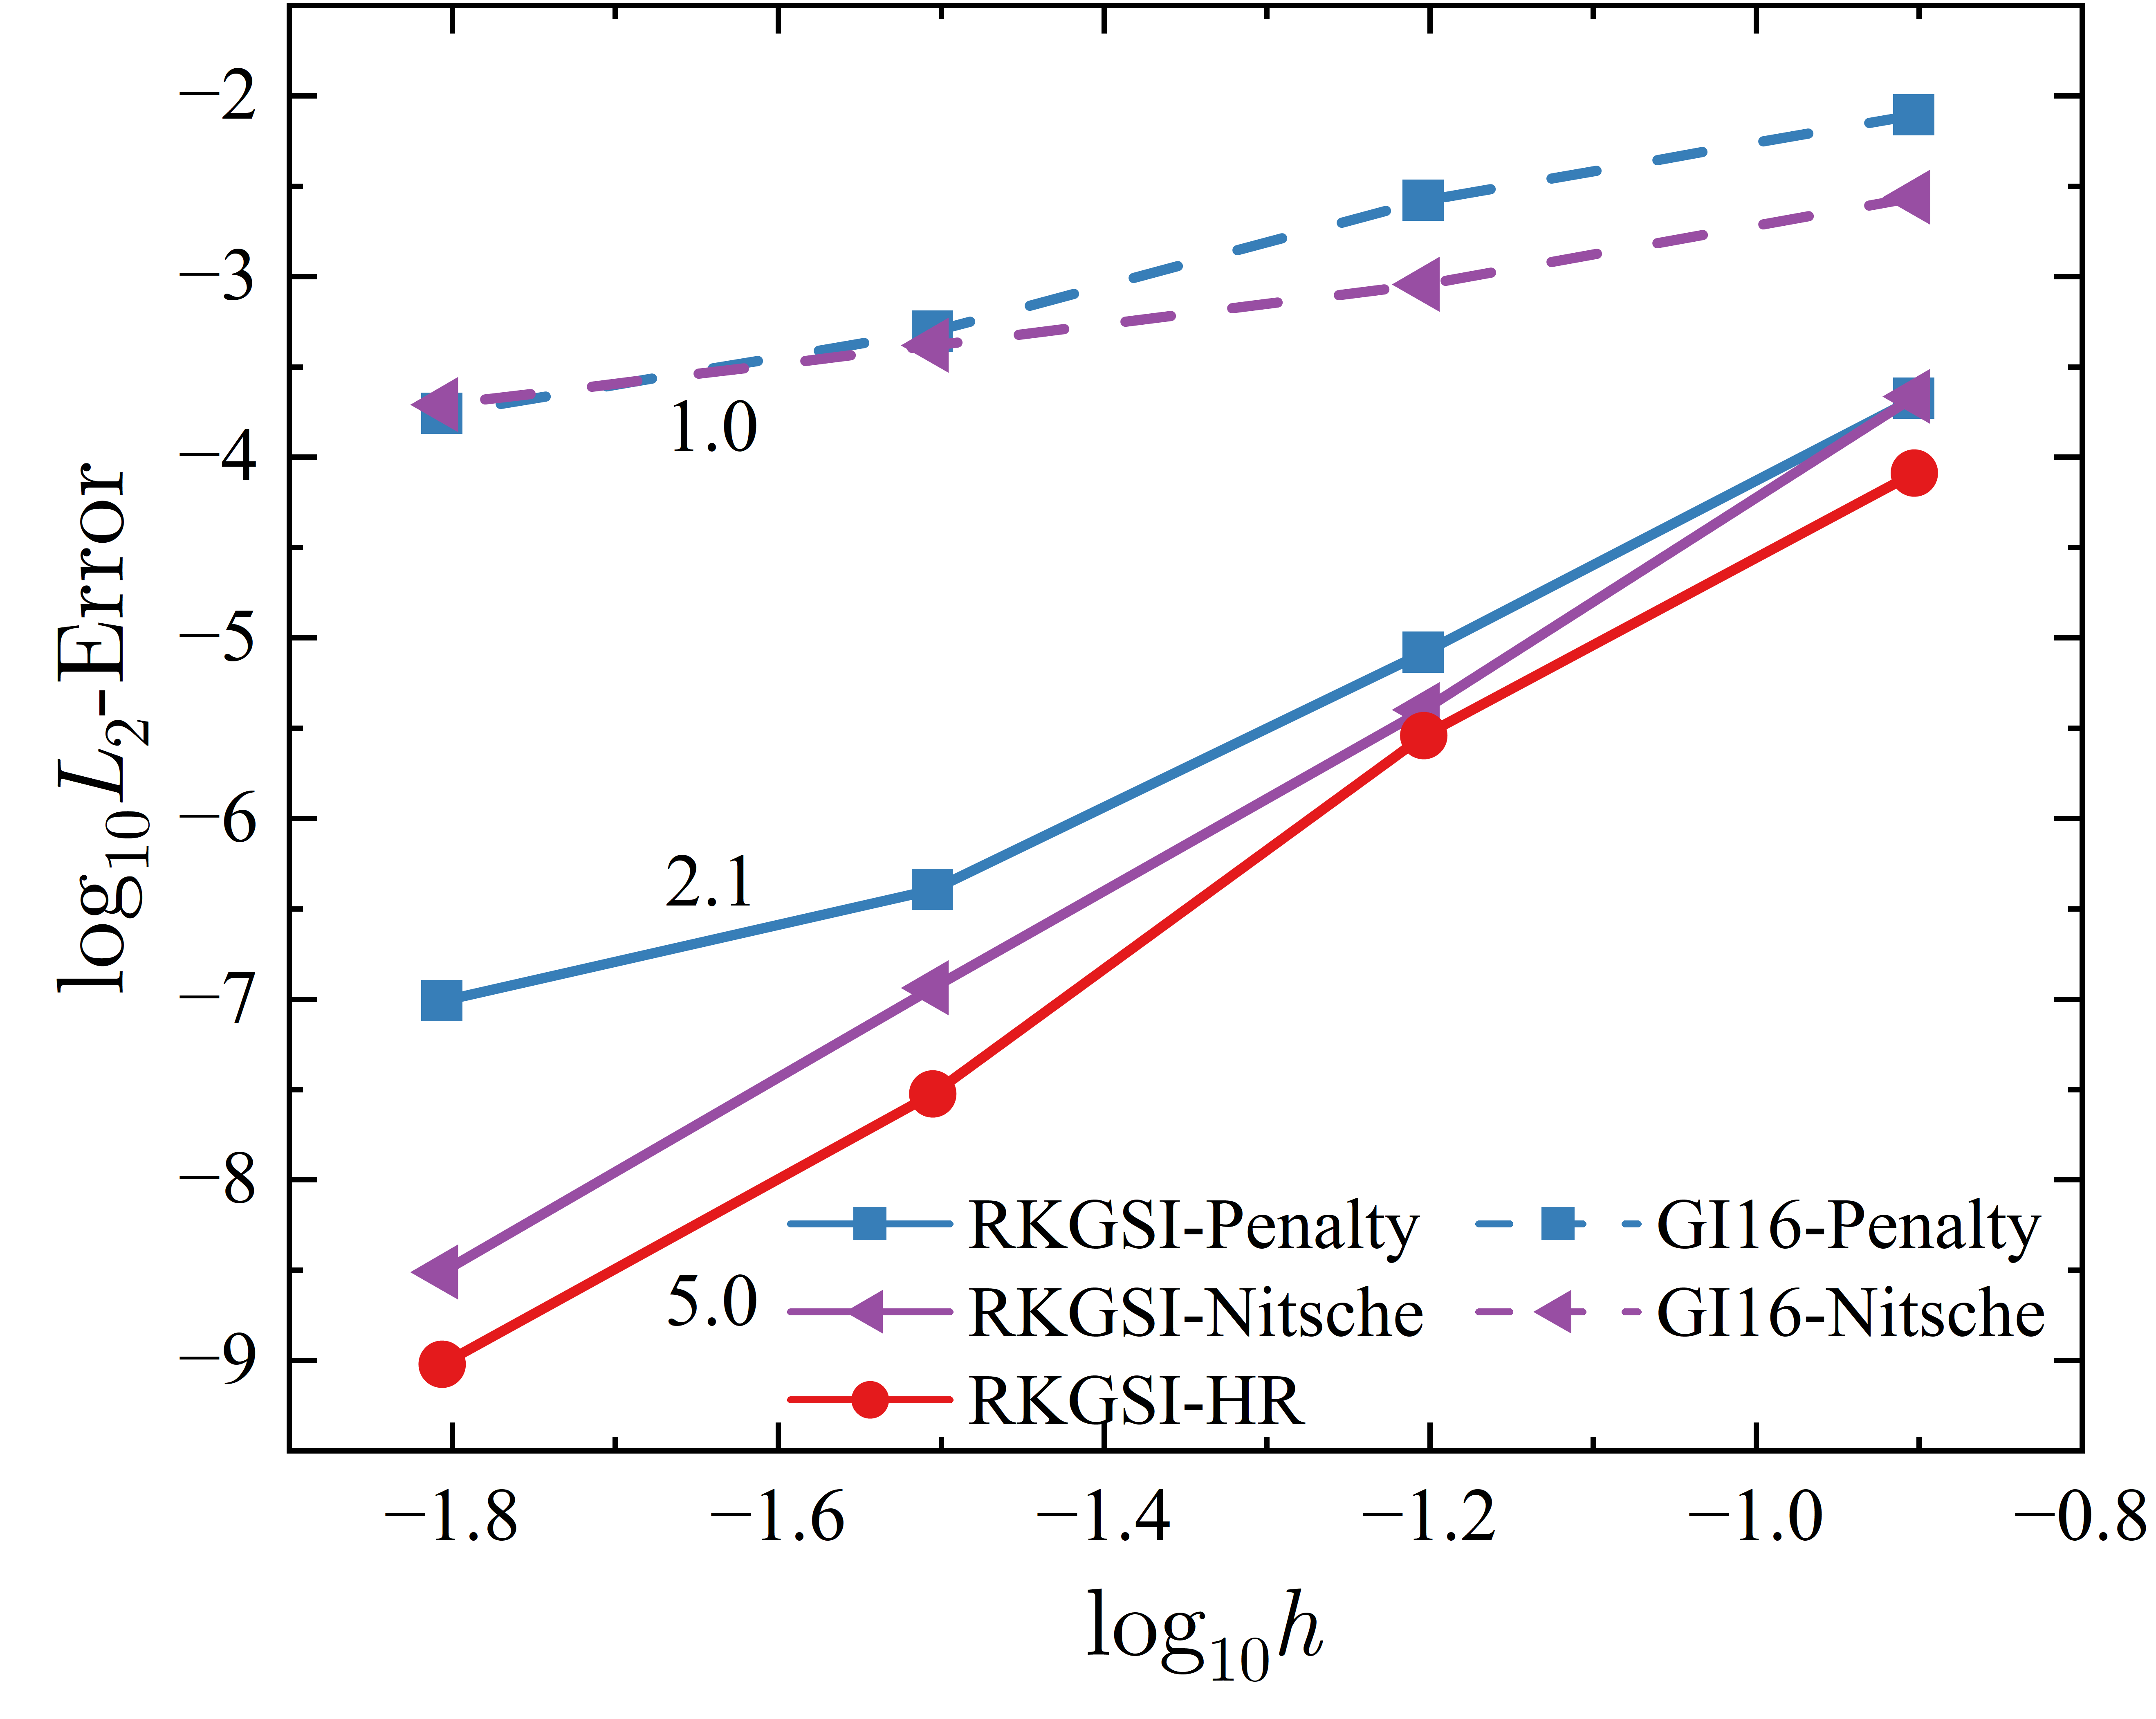
\includegraphics[width=0.49\textwidth]{figure/PHR/A/QL2.png}
    \phantomcaption\label{QL2}
    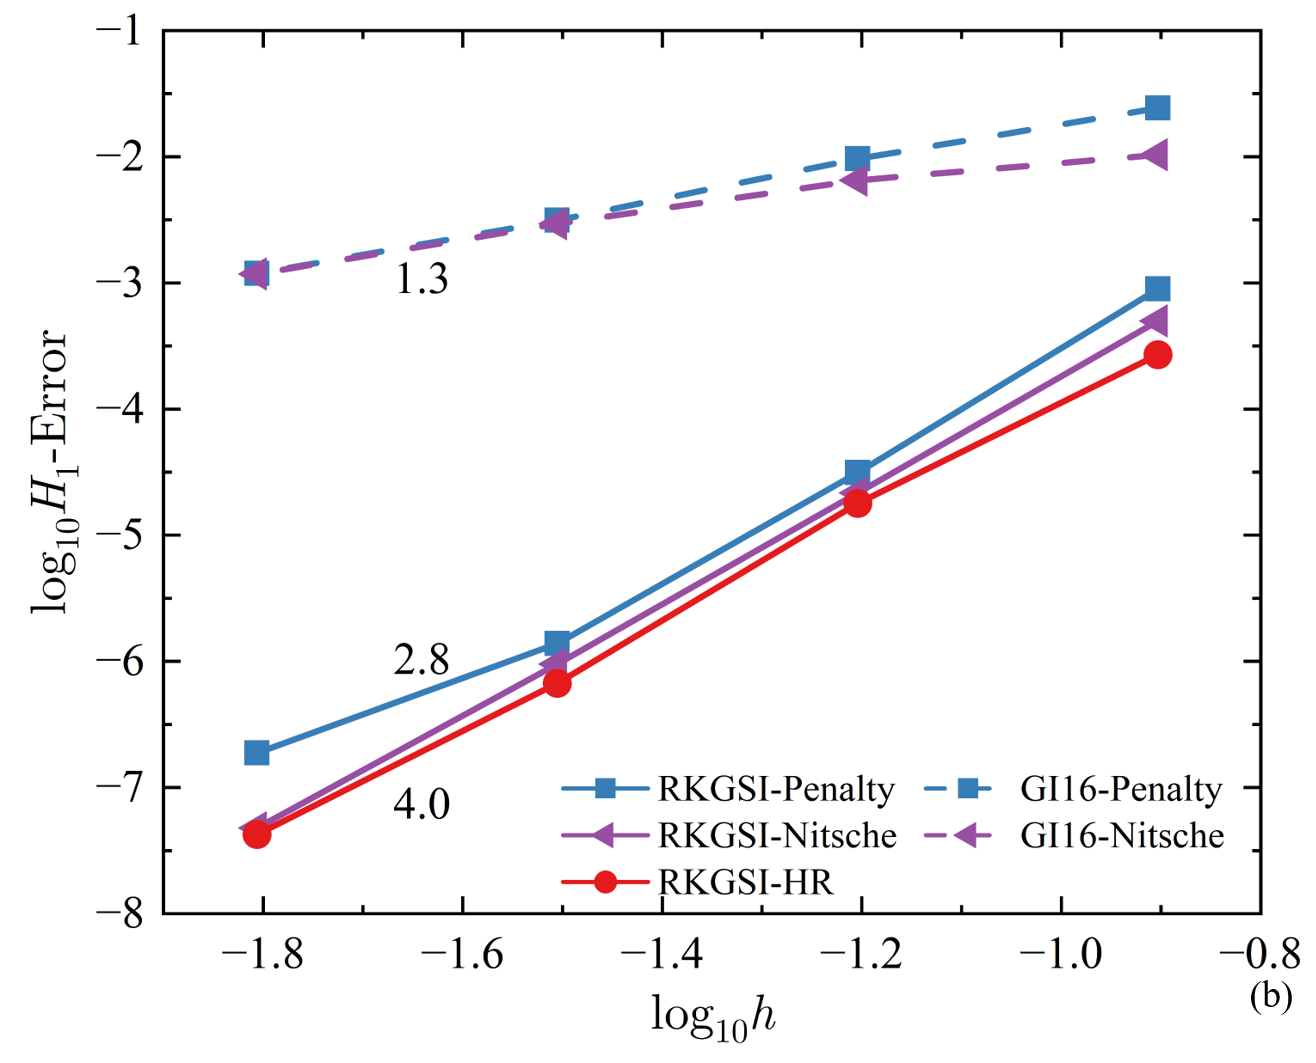
\includegraphics[width=0.49\textwidth]{figure/PHR/A/QH1.png}
    \phantomcaption\label{QH1}
    \end{subcaptiongroup}
    \begin{subcaptiongroup}
    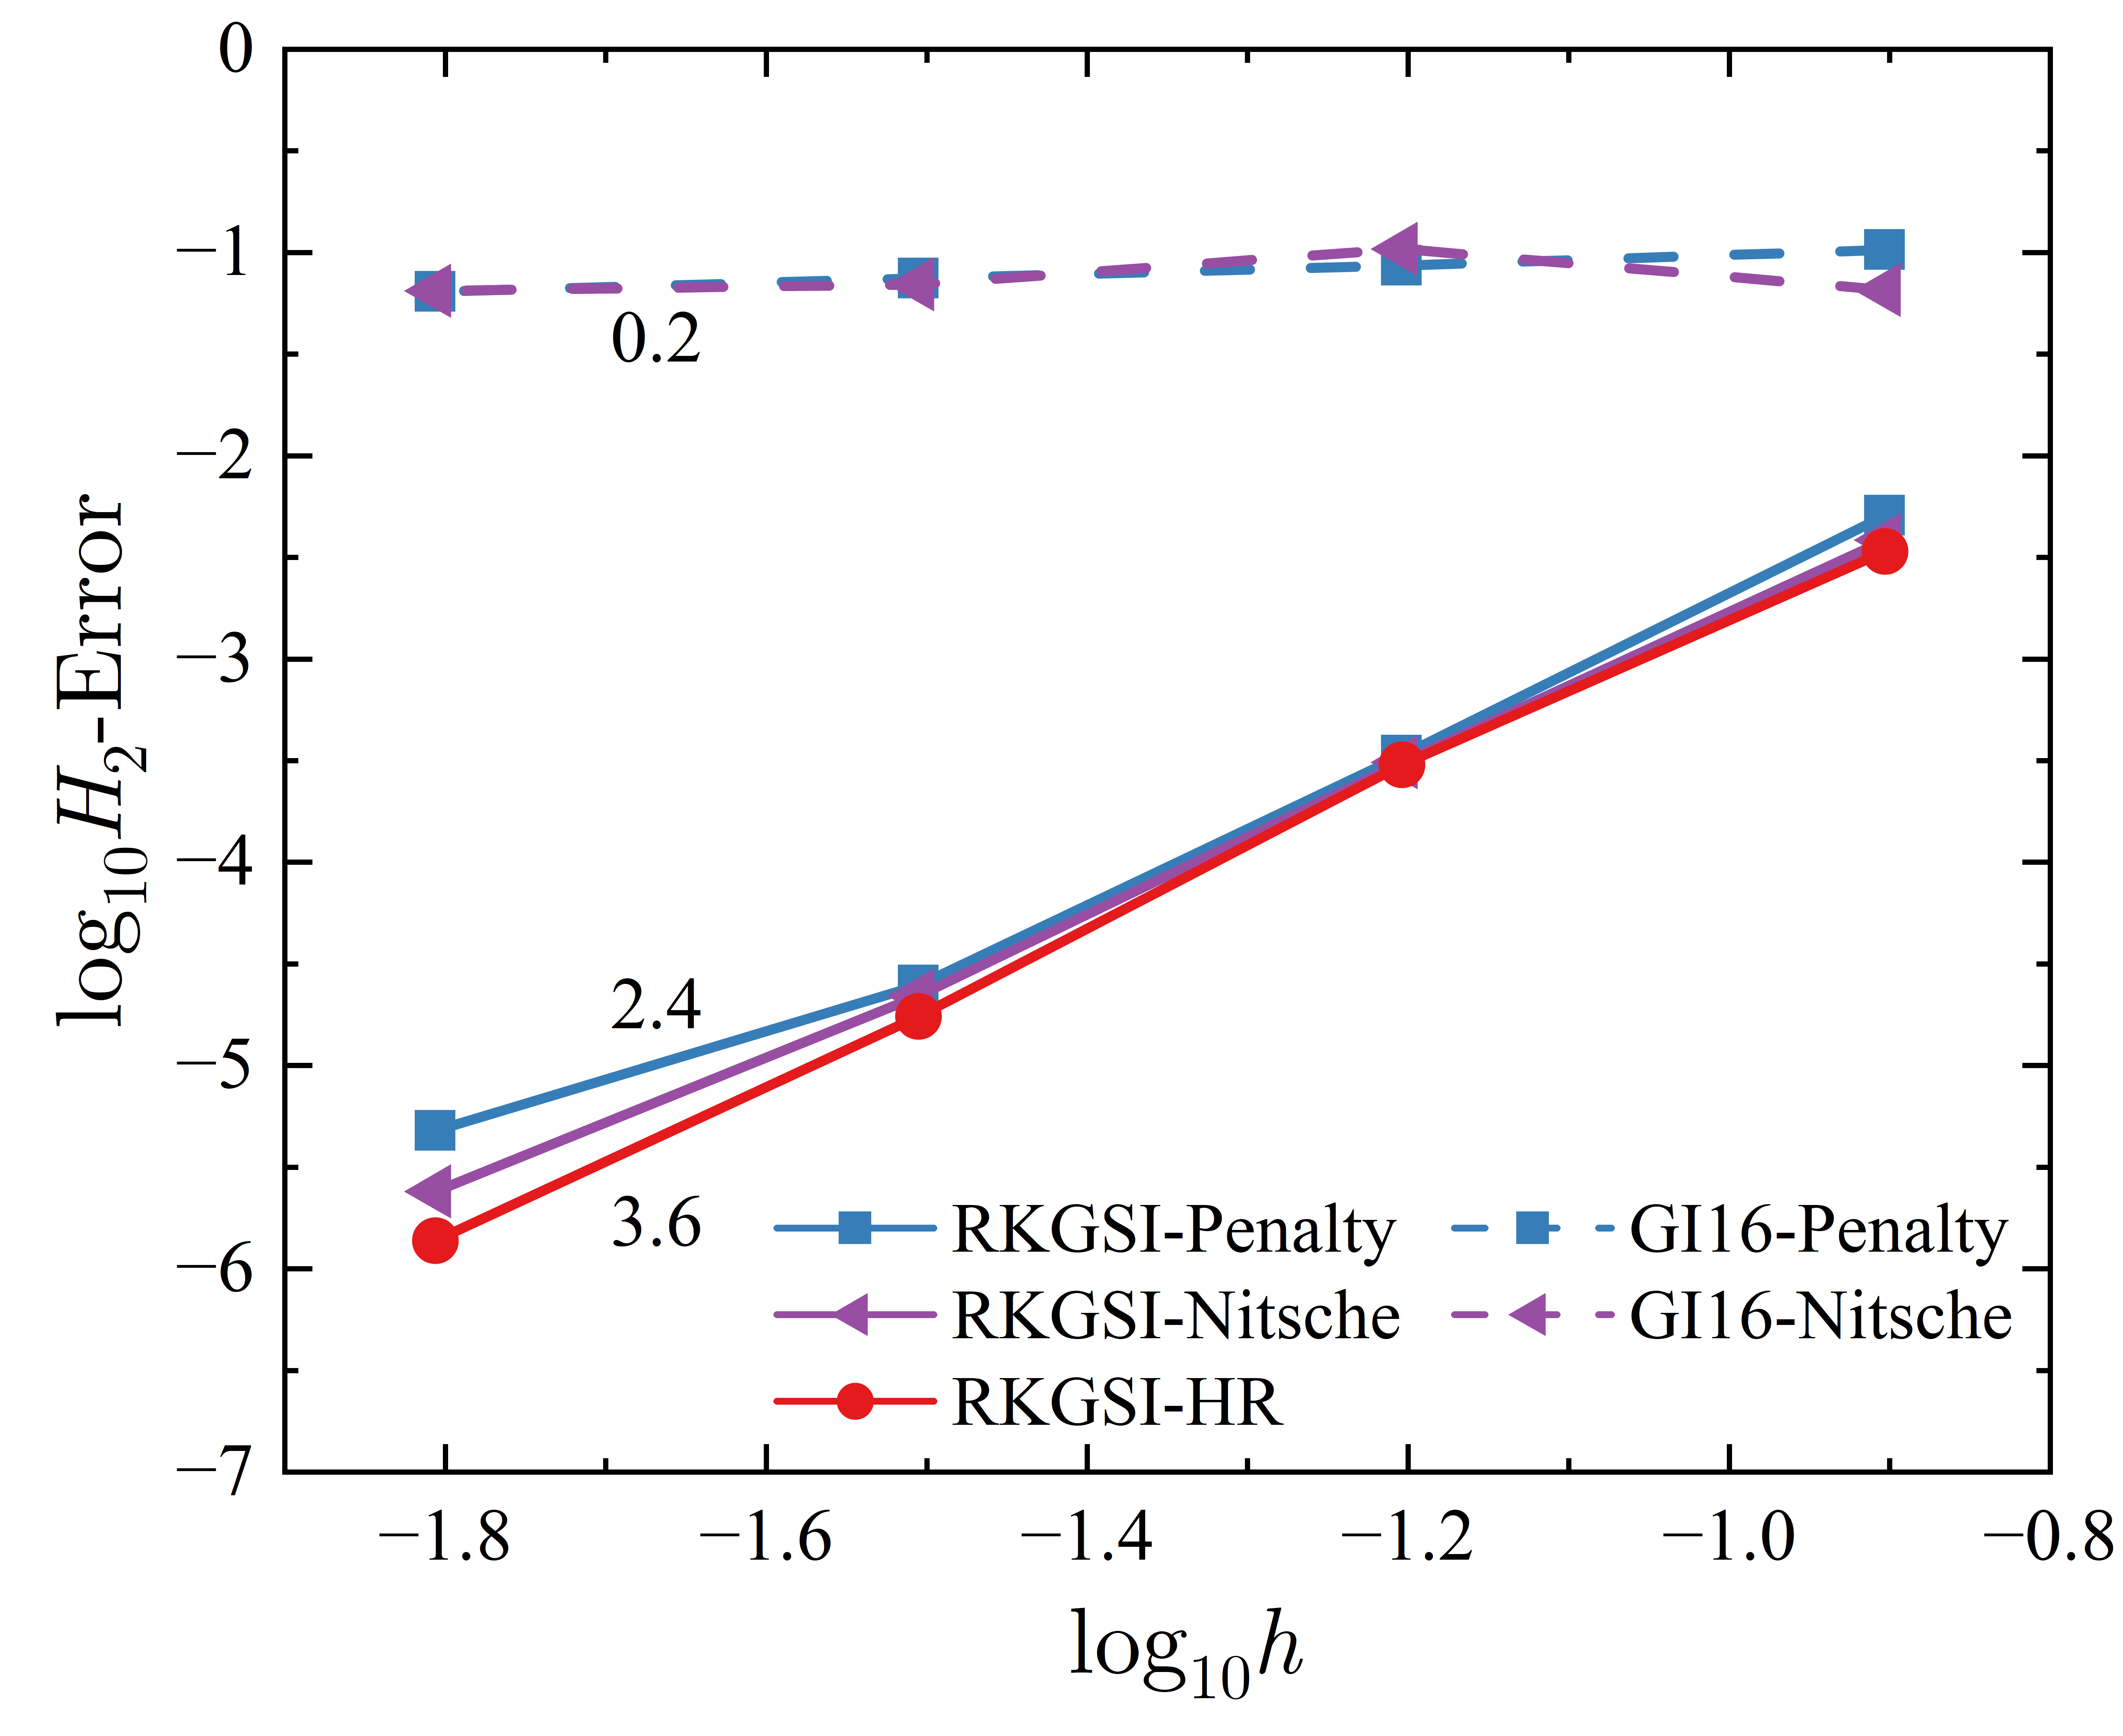
\includegraphics[width=0.49\textwidth]{figure/PHR/A/QH2.png}
    \phantomcaption\label{QH2}
    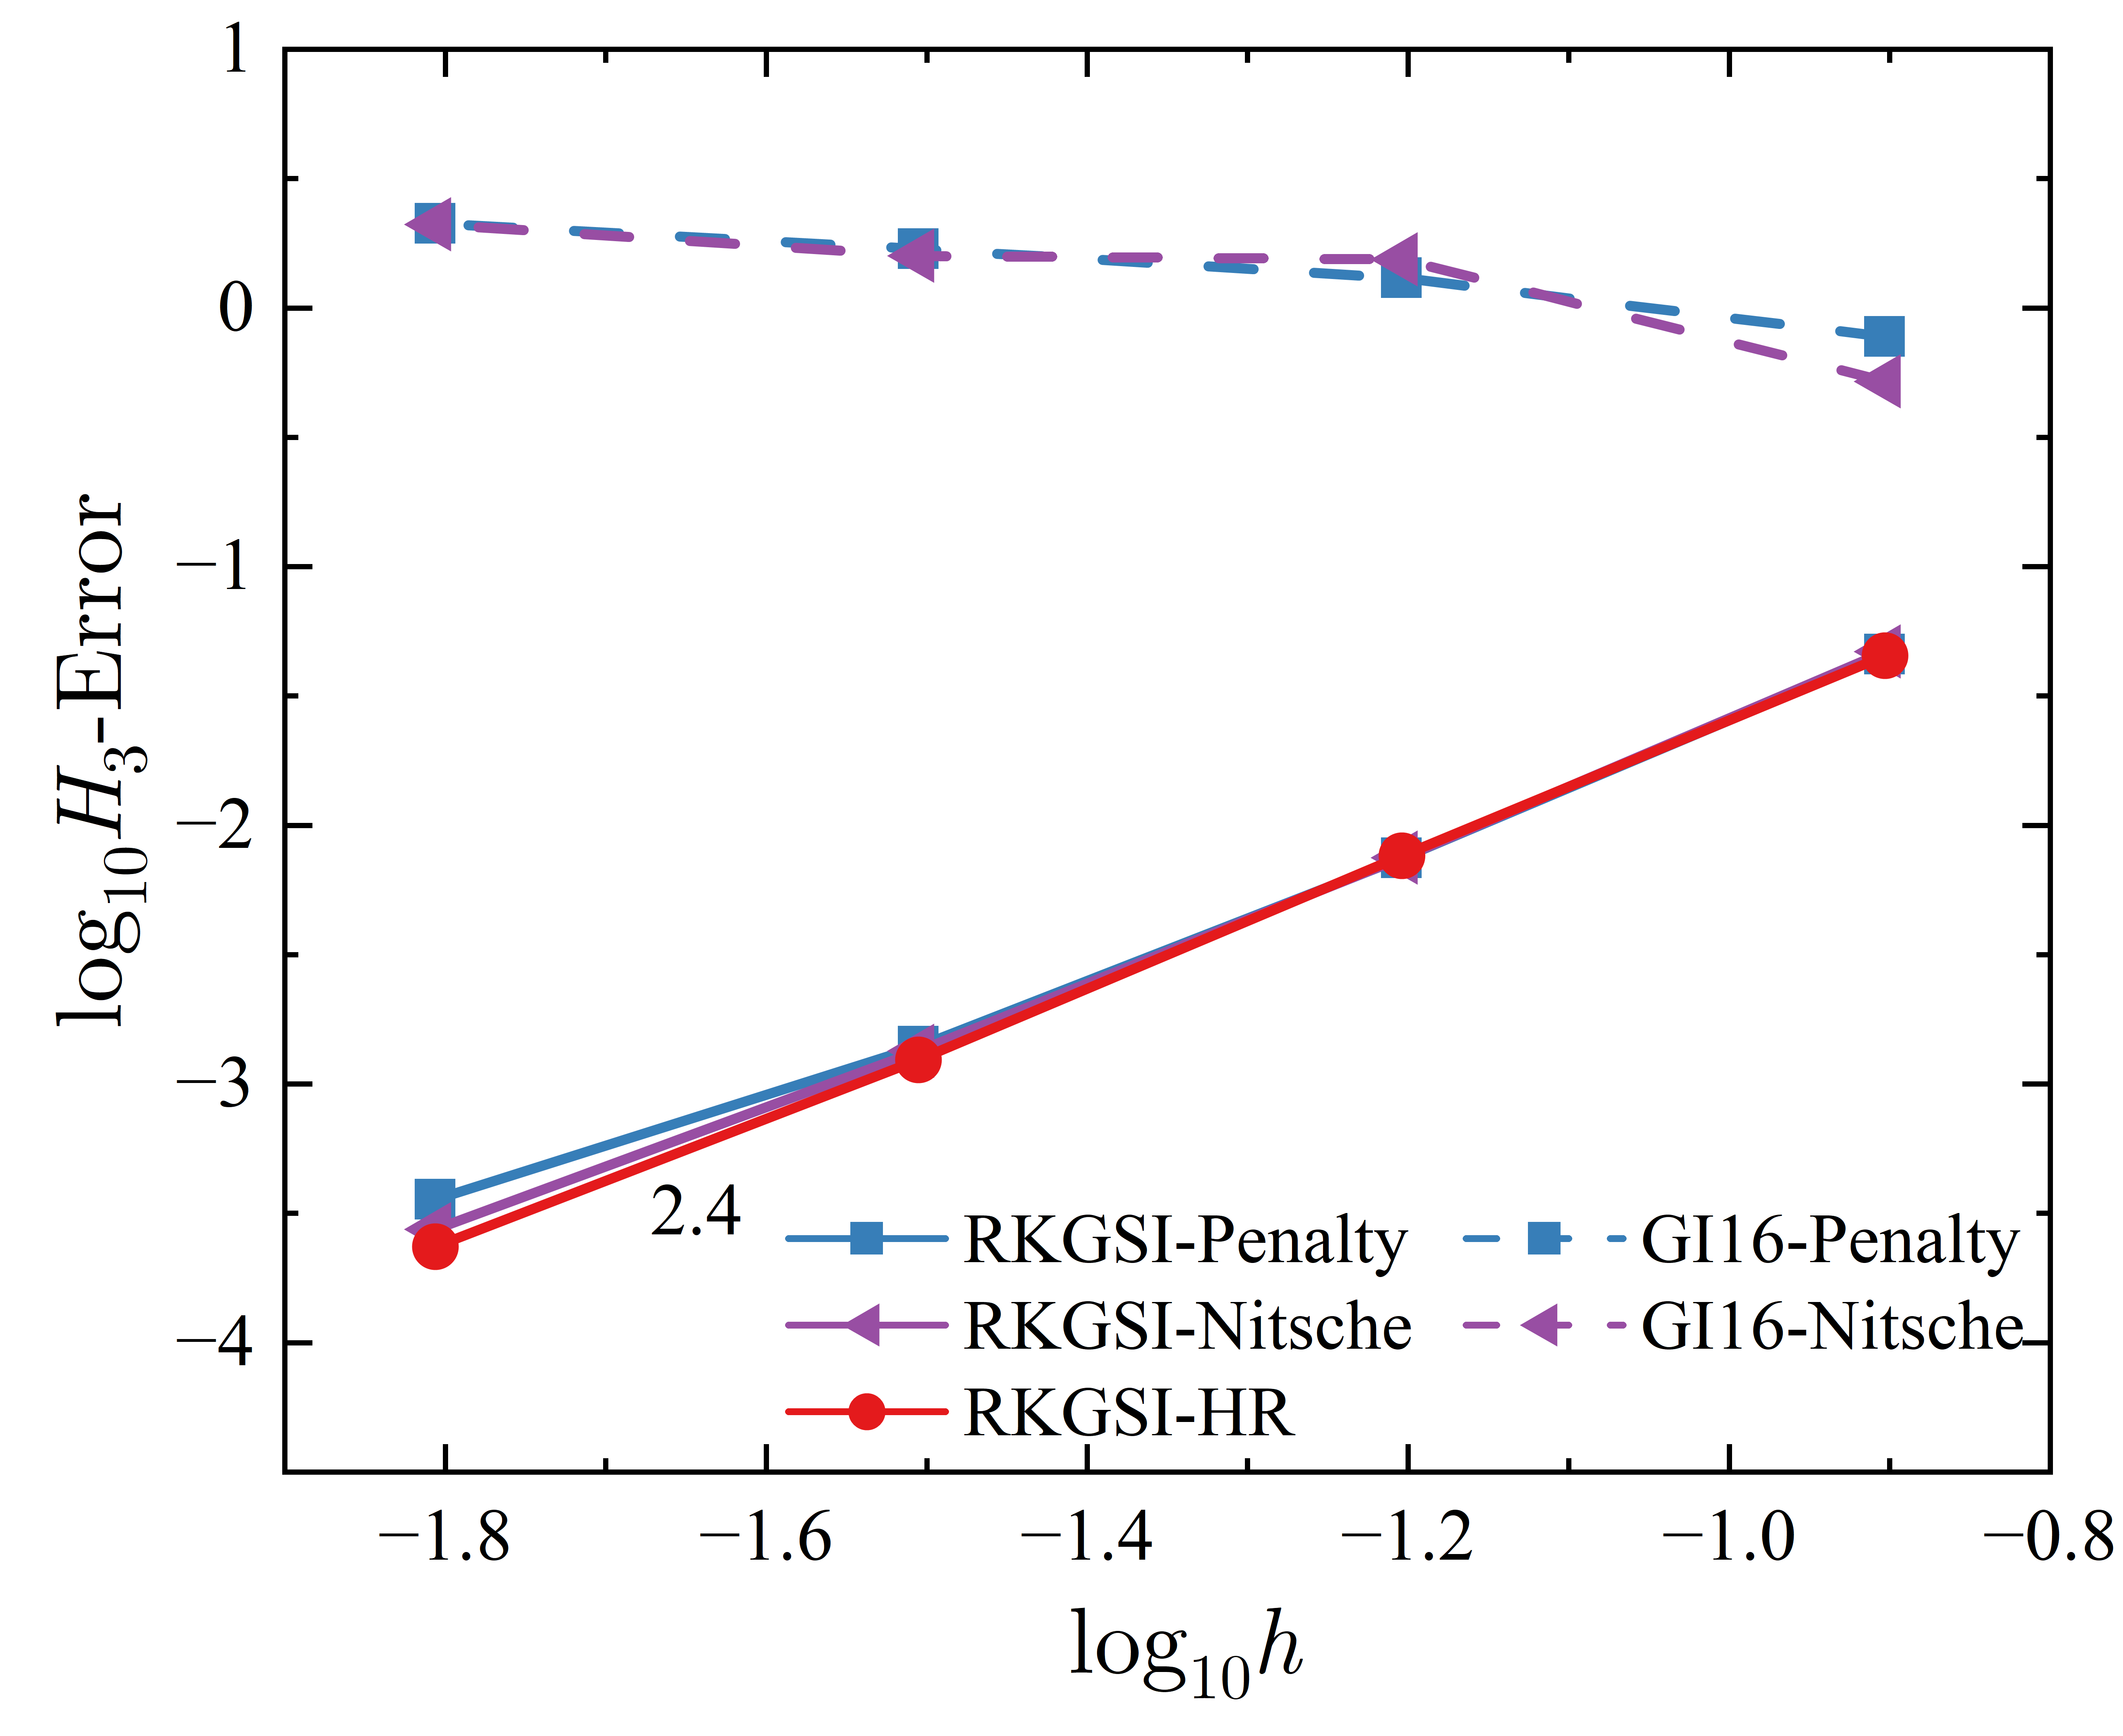
\includegraphics[width=0.49\textwidth]{figure/PHR/A/QH3.png}
    \phantomcaption\label{QH3}
    \end{subcaptiongroup}
\caption{简支环行板问题四次基函数误差对比:\subref{QL2} $L_2$误差;\subref{QH1} $H_1$;误差\subref{QH2};$H_2$误差;\subref{QH3} $H_3$误差}
\label{AQLH}
\end{figure}
\begin{figure}[H]
    \centering
    \begin{subcaptiongroup}
    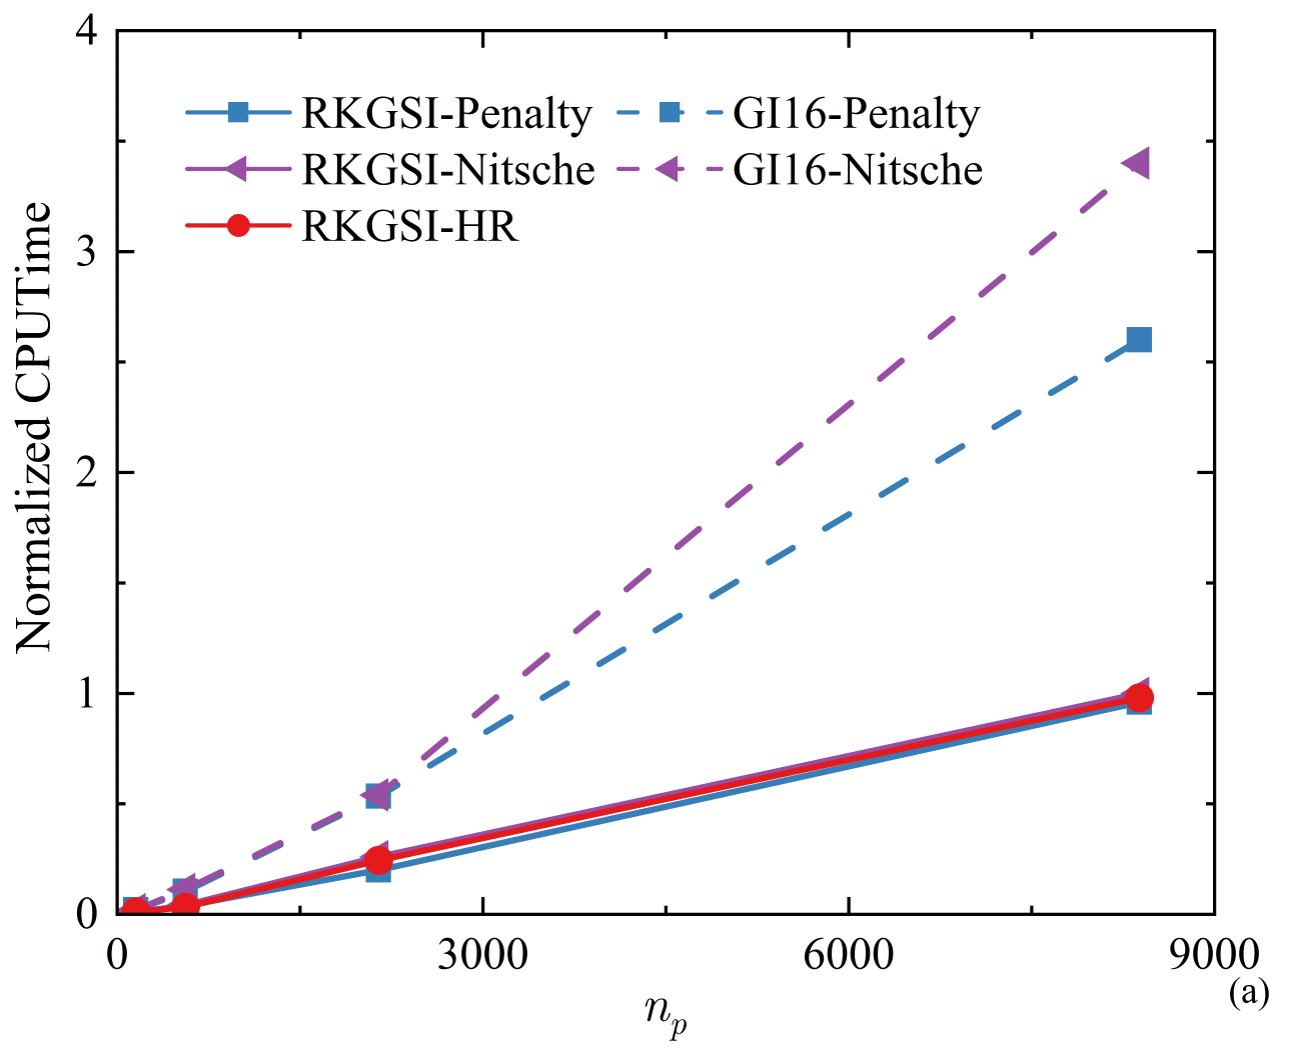
\includegraphics[width=0.49\textwidth]{figure/PHR/A/Qcputime.png}
    \phantomcaption\label{Qcputime}
    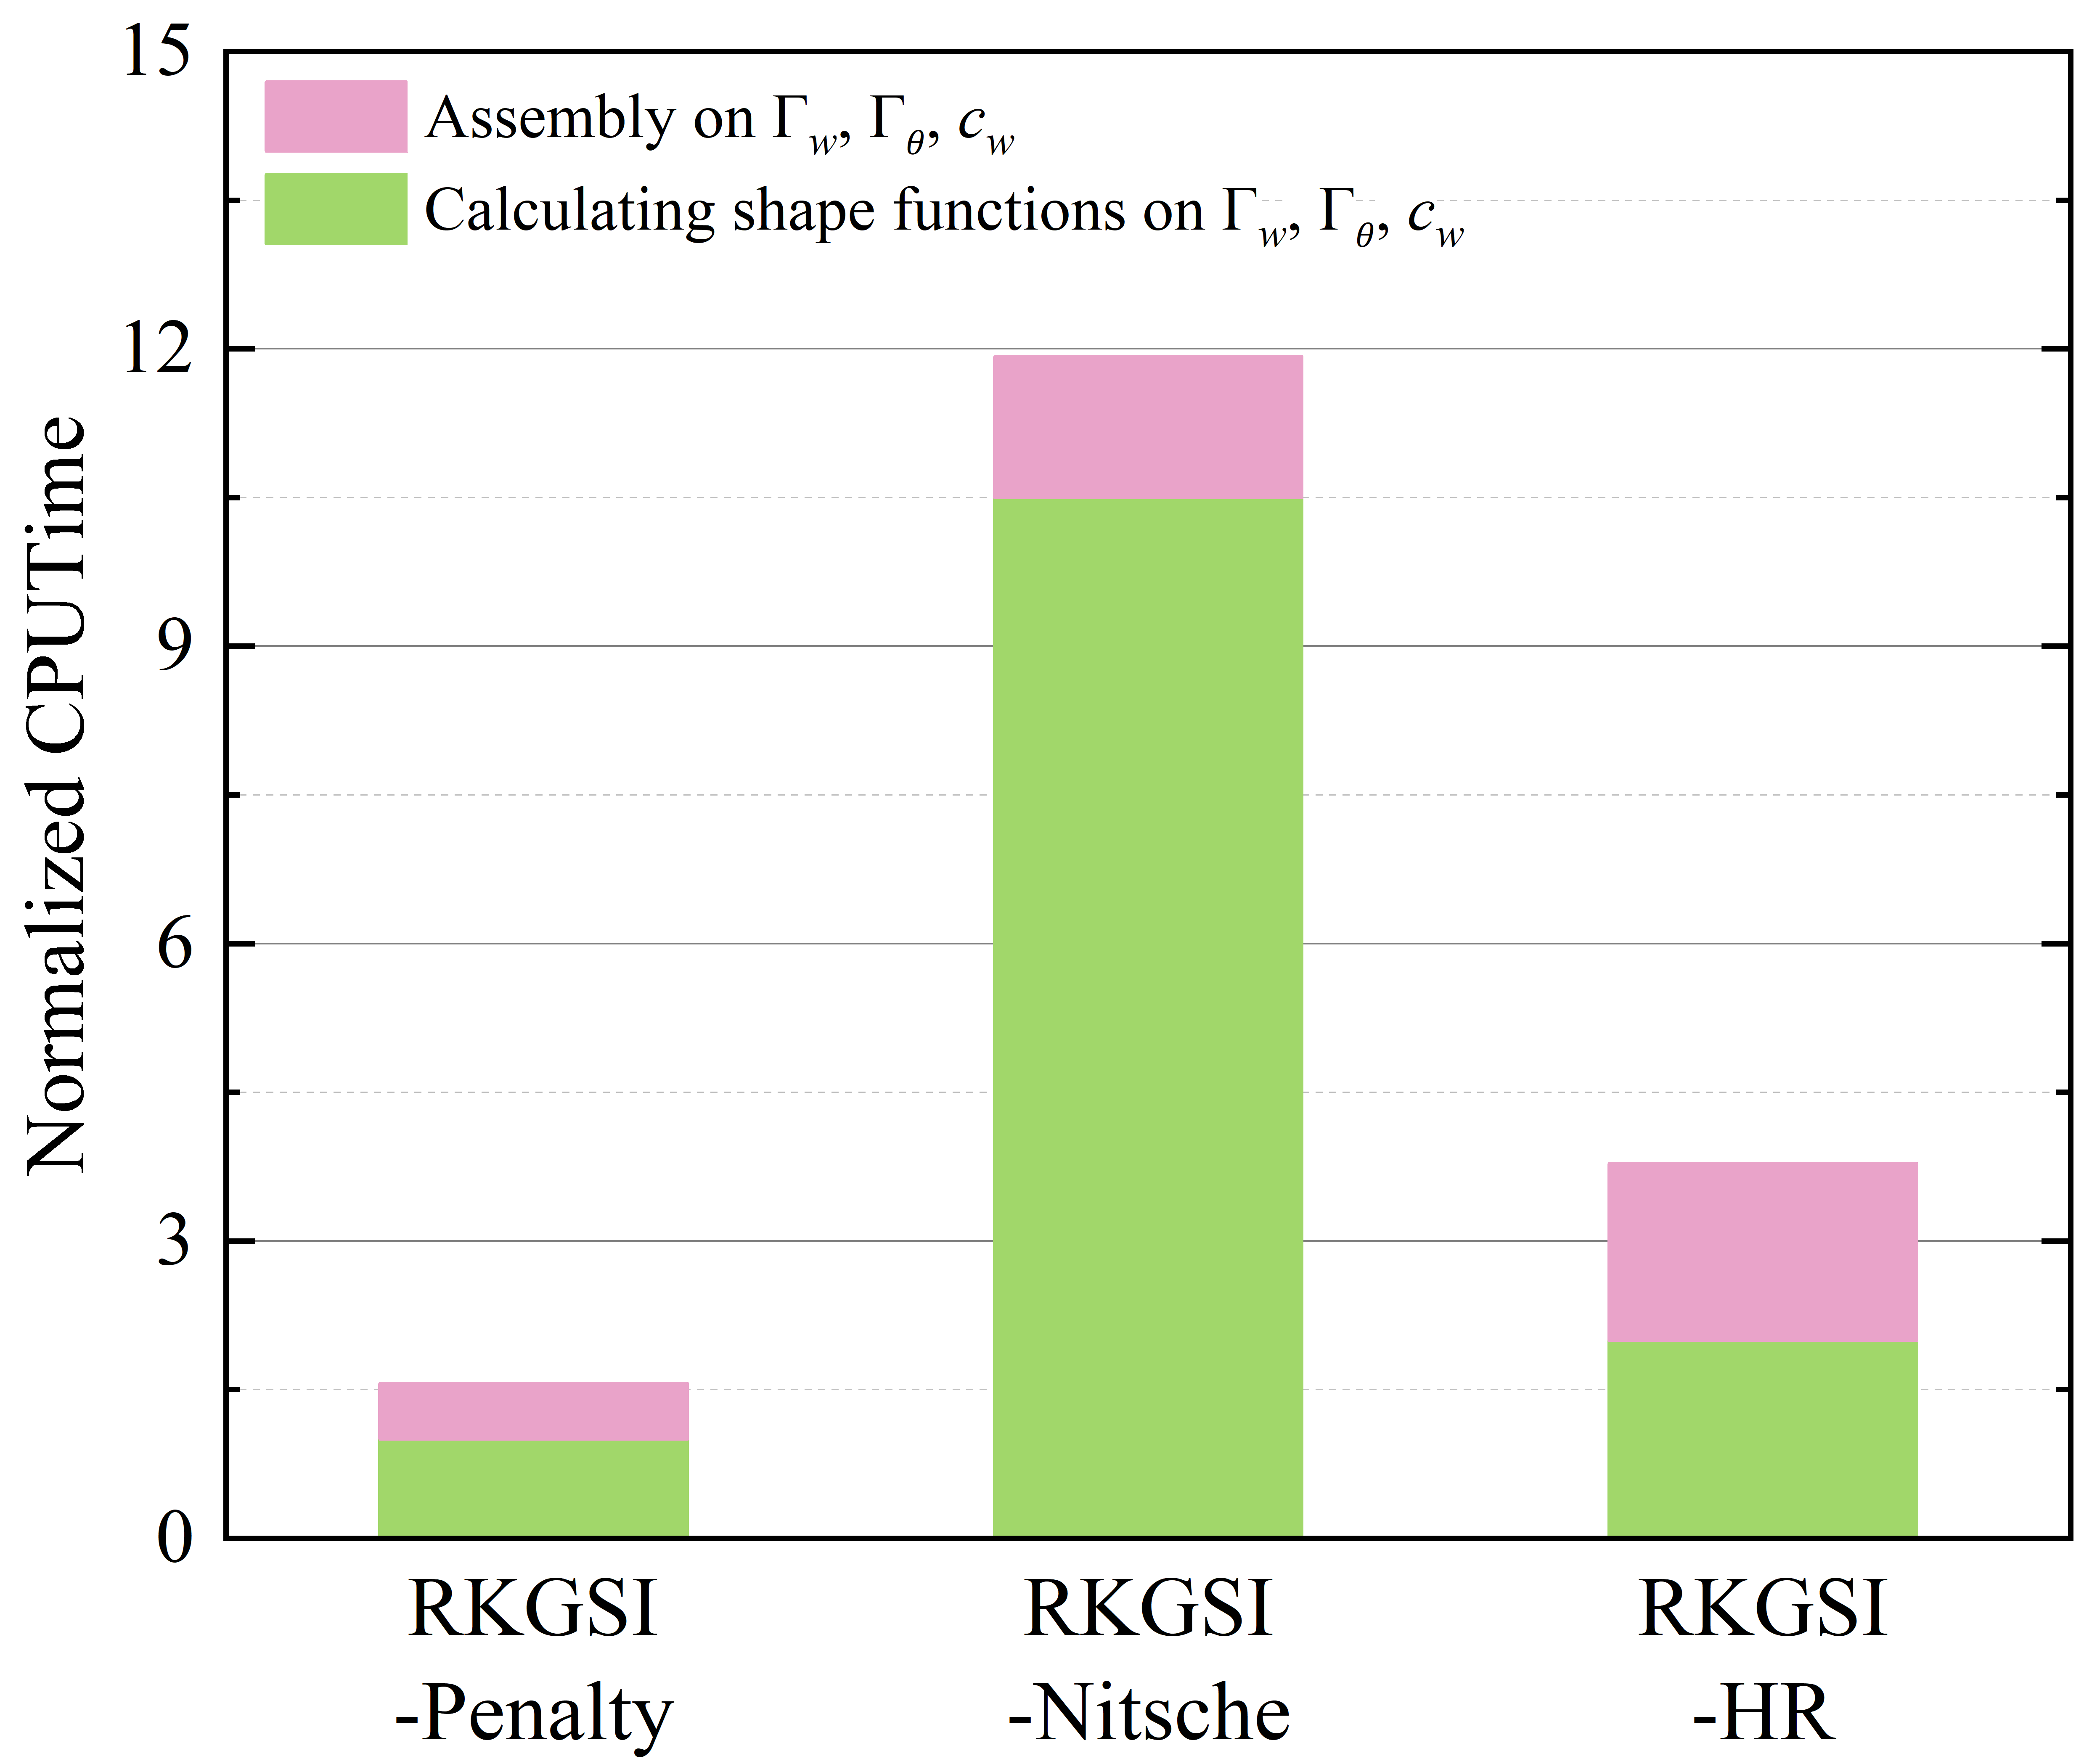
\includegraphics[width=0.49\textwidth]{figure/PHR/A/Qefficiency.png}
    \phantomcaption\label{Qefficiency}
    \end{subcaptiongroup}
\caption{简支环形板问题四次基函数效率对比:\subref{Qcputime}计算时间与节点数的关系;\subref{Cefficiency}本质边界条件施加效率分析}
\label{AQcputime}
\end{figure}
\section{小结}
本章进一步介绍了基于Hellinger-Reissner变分原理的变分一致性本质边界条件施加方法,用于求解薄板问题。
该方法通过采用混合离散近似Hellinger-Reissner变分原理弱形式中的挠度和弯矩,实现了满足积分约束条件用于求解高阶薄板问题的一种本质边界条件施加方法。
其中,在离散平衡控制方程中,采用传统无网格形函数对挠度进行离散,弯矩则在每个背景积分单元上以再生光滑梯度独立逼近。
通过采用再生光滑梯度积分法,该方法内嵌了局部积分约束条件,因此严格满足了每个积分单元的变分一致性。此外,由于二阶光滑梯度的计算只涉及无网格形函数及其一阶导数,有效的提高了计算效率。 
之后通过典型的数值算例进一步表明所提方法基于Hellinger-Reissner变分原理无网格薄板公式在满足变分一致性,计算精度以及计算效率方面优于采用传统高斯积分法的Nitsche法、罚函数法以及采用再生光滑梯度积分法的Nitsche法、罚函数法。
基于Hellinger-Reissner变分原理的变分一致性本质边界条件施加方法在解决薄板问题上提供了一种高效精确的边界条件施加方法。
\newpage
\begin{figure}[H]
    \centering
    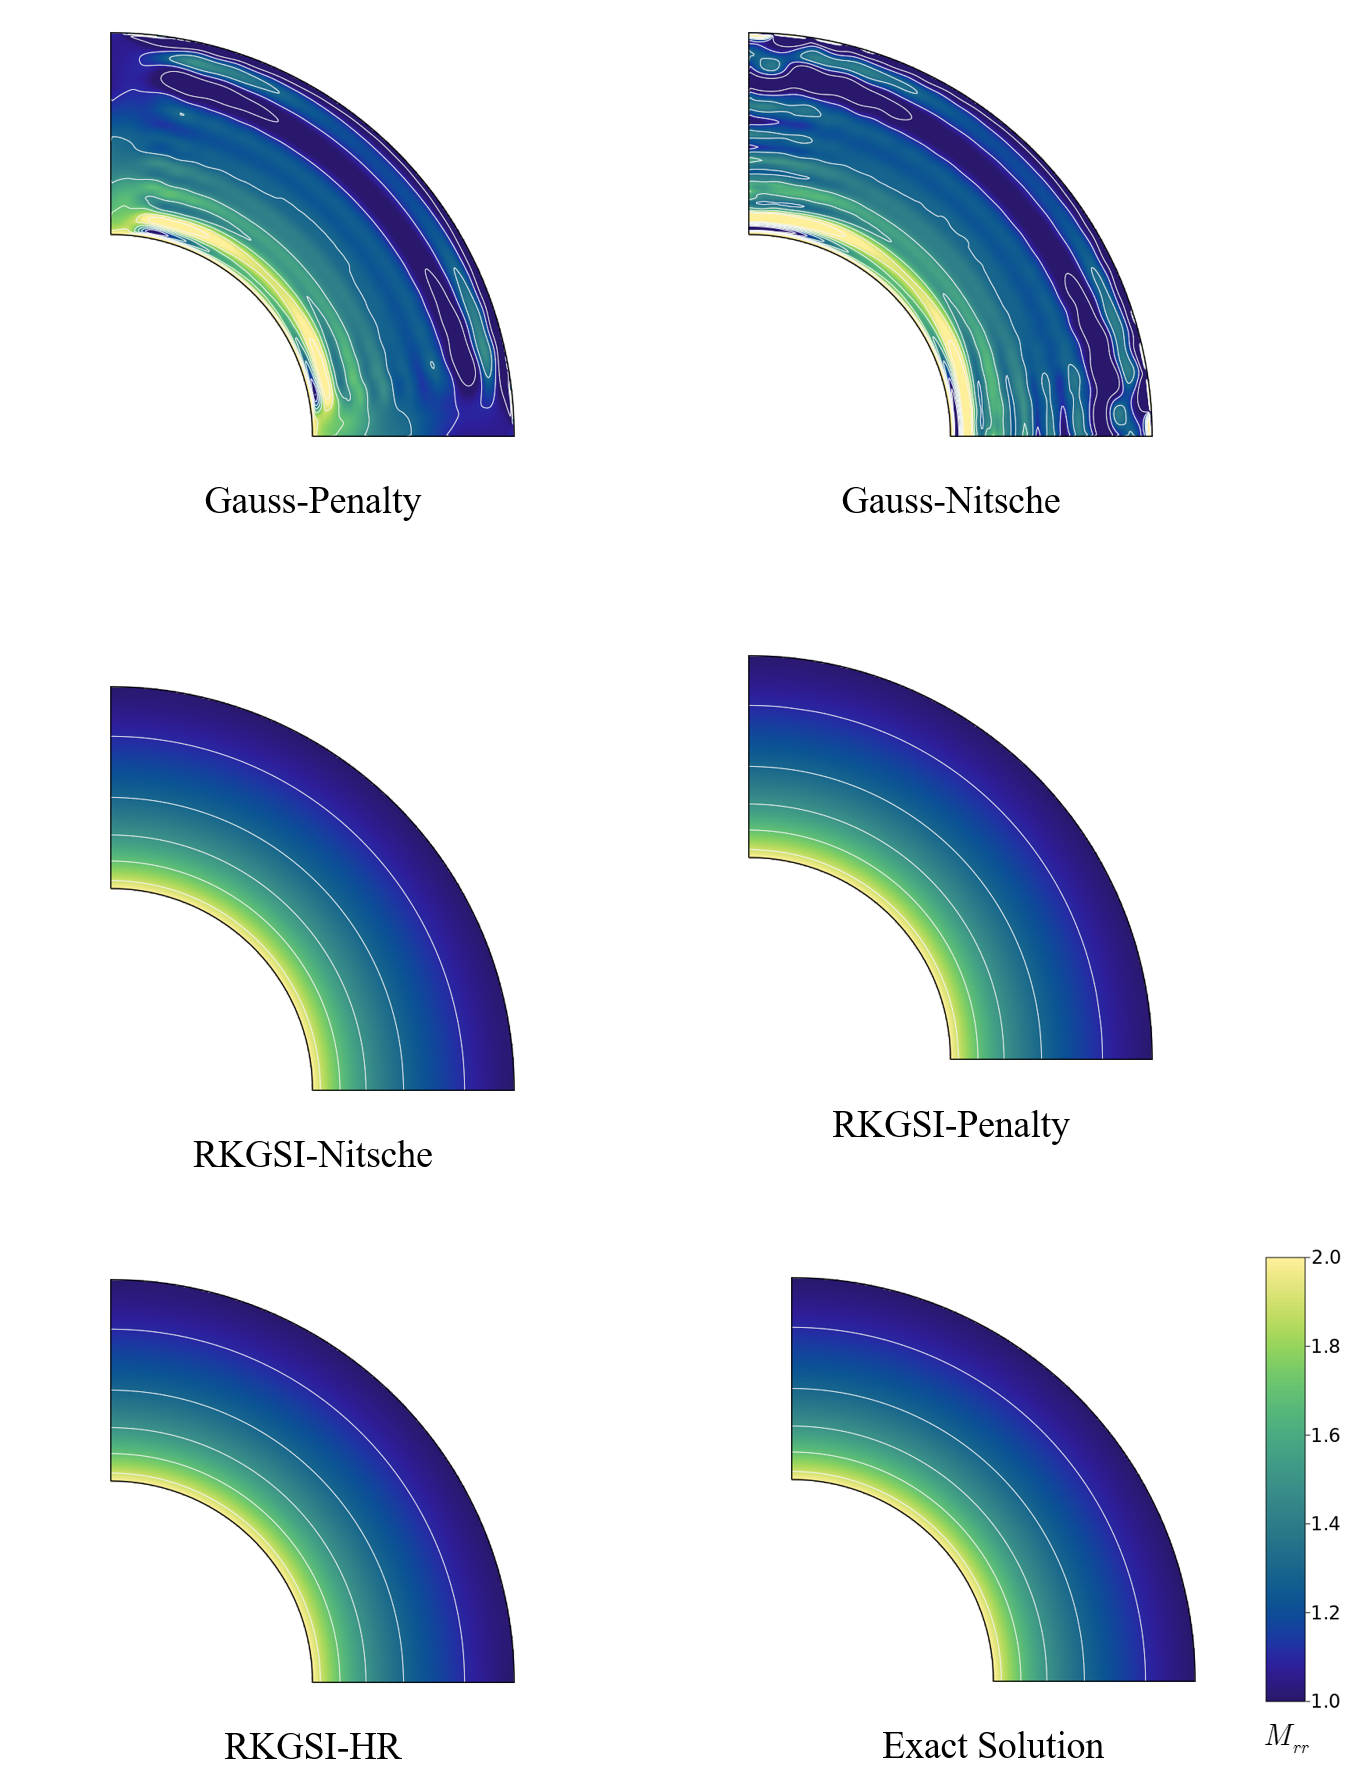
\includegraphics[scale=0.7]{figure/PHR/A/Mxy.png}
    \caption{简支环形板问题弯矩云图}\label{AMxy}
\end{figure}
\begin{figure}[H]
    \centering
    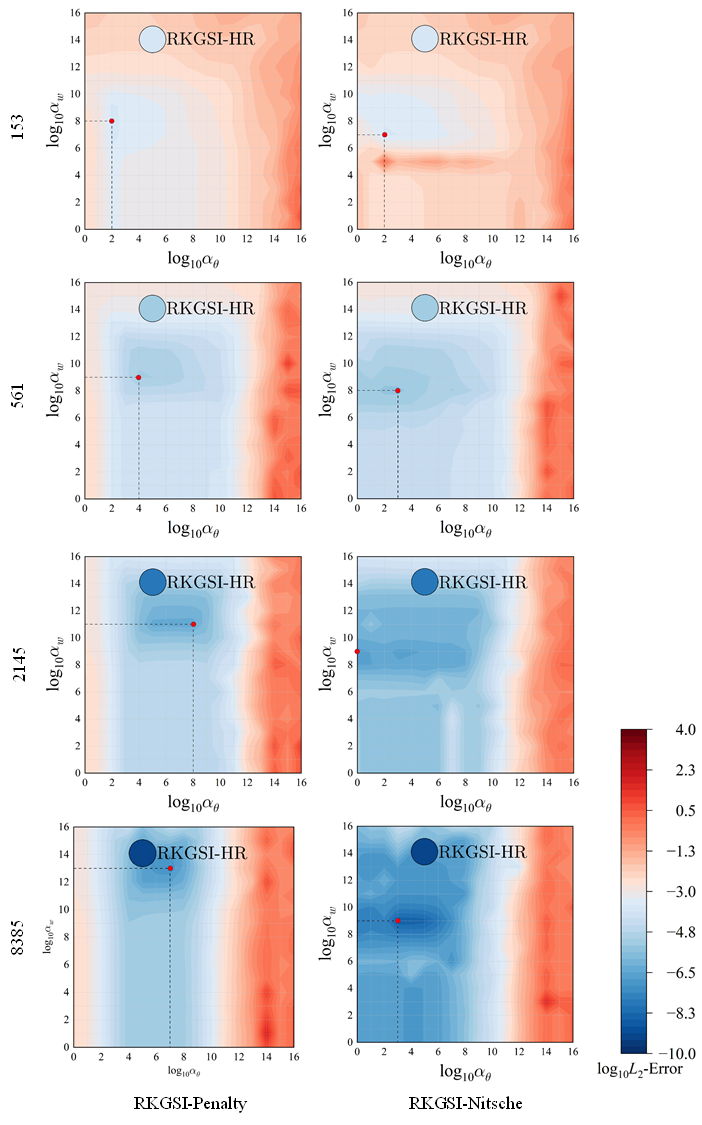
\includegraphics[scale=1.0]{figure/PHR/A/alpha.png}
    \caption{简支环形板问题人工参数敏感性分析}\label{Aalpha}
\end{figure}





